\chapter{Deployment and analysis of a low-background \bege~detector}
\label{chap:AnalysisBeGe}
	\section{Experimental setup}
	\label{sec:BeGeExperimentalSetup}

A 440~g \ppc~\textbf{B}road-\textbf{E}nergy \textbf{G}ermanium (\bege) detector manufactured by Canberra Industries was deployed underground on 24~August~2009 in the Soudan Underground Laboratory in Soudan, MN.  The purpose of the deployment of this detector was to obtain low-threshold, low-background counting data to seek improved limits on WIMPs in the low-mass range ($\lesssim10$~GeV).  The design of this detector included several custom modifications to address backgrounds seen with a previous \ppc~used to obtain dark matter limits~\cite{Aalseth:2008aa}, including several internal mounting components replaced by ones constructed with cleaner materials by J.~Collar at the University of Chicago.  A summary of relevant geometrical aspects of the detector is provided in Table~\ref{tab:BEGeCharacteristics}.
% Additionally, the outer cryostat was not made of typical aluminum but rather of copper.  True?
The detector was placed in the same shield as described in Section~\ref{sec:DeploymentPPC2SoudanIntro} with a few small changes.  The inner OFHC copper shield was replaced by old Pb bricks from the University of Chicago and a different PMT-based muon veto was placed around the external borated polyethylene shield.   %FixME contamination of bricks?

			\begin{table}
				\centering
				\begin{tabular}{l r}
					\toprule
					Property & Value \\
					\midrule
					Manufacturer & Canberra \\
					Mass & 440 g \\
					Outer diameter &  60.5~mm\\
					Length &  31~mm\\
					Active Volume & 83.4~cc \\
					Capacitance & 1.8~pF (@3000~V bias) \\

					\bottomrule
				\end{tabular}
				\caption[\bege~detector characteristics]
				{\bege~detector characteristics.  }
				\label{tab:BEGeCharacteristics}
			\end{table}

This chapter presents results from data taken with the BeGE detector underground from the time period beginning 4 December 2009 until 15 May 2010 for a total live-time of 150.6~days.  During this time, there were two main gaps in run time, including a roughly 5-day shutdown period during a planned power outage at the lab and another 6-day period during which parameter settings for the DAQ were modified.  Results from a parallel analysis of a previous subset of the data occupying about 2 months of live-time have been presented in~\cite{Aalseth:2010aa}.

	\section{Data acquisition and processing}
	\label{sec:BeGeDAQProcessing}
	
The DAQ system used was similar to the one used in~\cite{Aalseth:2008aa}.  The preamp of the \bege~included 2~signal outputs, an inhibit output generating a logic signal when the reset circuitry of the preamp was active, and a test input for waveform generator pulses.  The initial system was set up without the ability to digitize raw preamp traces, but a later upgrade on 1~Dec~2009 introduced additional hardware to take this data.  The readout system was a PCI-based National Instruments digitizer with 6~channels, sampling at 20~MS/s with a resolution of 8~bits.  This digitizer allowed selectable voltage ranges, enabling higher resolution at lower energies.  The acquisition software used was a Windows- and Labview-based program designed by J.~Collar.  

One of the preamp signal outputs was run into an analog spectroscopy amplifier with a 10$\mu$s shaping time.  Two outputs from this amplifier were input into the digitizer with different voltage ranges: -0.05$\to$0.05~V (high gain) and -0.25$\to$0.25~V (low gain).  The second preamp output was AC-coupled to a Phillips Scientific 777 fast (DC$\to$200~MHz) amplifier using a capacitor to yield a $\sim$50~$\mu$s decay time.  This stage provided a $\sim1\times$ gain and was used as a fan-out for two outputs to the next stage: (1) one output was input into a spectroscopy amplifier with 6~$\mu$s shaping time and then into the digitizer; (2) the other output was sent to another gain stage of the 777.  The two outputs from the fan-out of this stage were then input into two channels of the digitizer with different voltage ranges: -0.05$\to$0.05~V (high gain) and -0.25$\to$0.25~V (low gain).  The 777 allowed adjustment of the output offset, and so the baseline was set to be close to the upper maximum of the high-gain channel.  This was to maximize the dynamic range for digitizing the negative-going preamplifier pulses.  

The muon veto was composed of 10~flat panels situated around the outside of the polyethylene shield, with 6 on the sides and 4 covering the top.  The outputs of all the panels were coupled together and reduced to one channel, effectively OR-ing all the PMTs.  This single channel was then input into a discriminator with a threshold set to output logic pulses when any of the PMTs registered a single photon event and the logic output was input into the last remaining channel of the digitizer.  The outputs read into the DAQ system are detailed in Table~\ref{tab:SoudanDAQTable}.  All channels were digitized at 20~MHz with 8 bits, and each trace length was 8000 samples (400~$\mu$s) long.  The level-sensitive trigger was generated by the high-gain, 6~$\mu$s-shaped, channel~0.  When a pulse exceeded the trigger level in channel~0, all 6 channels were read out.  

	\begin{table}
		\centering
		\begin{tabular}{l c}
			\toprule
			Channel & Characteristics \\
			\midrule
			0 & High-gain (0-3.5~keV), 6$\mu$s shaping, triggering \\
			1 & High-gain (0-3.5~keV), 10$\mu$s shaping \\
			2 & Low-gain (0-14~keV), 10$\mu$s shaping \\
			3 & Muon-veto \\
			4 & High-gain, AC-coupled preamp trace (unshaped) \\
			5 & Low-gain, AC-coupled preamp trace (unshaped) \\
			\bottomrule
		\end{tabular}
		\caption[DAQ Channel readout characteristics]
		{DAQ Channel readout characteristics. }
		\label{tab:SoudanDAQTable}
	\end{table}

The inhibit output from the preamp was used as an online veto by splitting the inhibit signal and using the `INHIBIT' inputs on the spectroscopy amplifiers.  When the logic is active on this INHIBIT input, the spectroscopy amplifier maintains the baseline of its output, effectively removing any trigger generated by a reset of the preamp.  It should be noted that, in contrast to the DAQ system described in Section~\ref{sec:DeploymentPPC2SoudanDAQSystem}, no timing information of the inhibit pulse was retained to perform a later estimate of dead-time.  Instead, during detector deployment it was found that the reset pulse rate was stable at $\lesssim$3~Hz, suggesting that differences in temperature did not affect this setup as profoundly as \ppc2 (see Section~\ref{sec:DeploymentPPC2SoudanAnalysisCuts}) or that the detector cold finger was more properly coupled to the liquid nitrogen.  This stability was further confirmed by a measurement of the baseline vs.~time detailed in Section~\ref{sec:BeGeParsVsTime}.
A 1~ms veto following the pulse reset then produces a less than 0.3\% reduction in live-time, which is ignored.  %FixME Found out if JO still sees this at PNNL.

	The digitizer card maintained an internal buffer to store a set of events.  After 20~events were stored, data from the digitizer buffer were written to disk and file names were cycled (open file closed, saved, and new file opened) every 3 hours.  An automatic data management chain was setup similar to that described in Section~\ref{sec:DeploymentPPC2DataProcessing} with a run database used to facilitate the data processing.  Files were synchronized back to a server at the University of Washington where they were persisted on RAID-ed disks.  Once a file appeared on the UW server, a corresponding record was introduced into the database and this record was used to control and track further processing.  The processing progressed in a tiered fashion as follows:
		\begin{enumerate}
			\item[Tier 0:]  Raw data from the Labview DAQ system
			\item[Tier 1:]  ROOTified data - raw data converted to MGDO objects and stored in ROOT TFiles
			\item[Tier 2:]  Waveform processed data - extraction of waveform characteristics using MGDO Transforms
		\end{enumerate}
Details on the waveform processing are given in the following Sections: \ref{sec:BegeShapedProc}, \ref{sec:UnshapedWFProc}, and~\ref{sec:MuonProc}.  For more details regarding the MGDO objects and the framework of the analysis chain, see Appendix~\ref{app:MGDO}.
	
		\subsection{Shaped channel processing}
		\label{sec:BegeShapedProc}

The shaped channels (0, 1, and 2) were processed to extract amplitude information of the pulses.  These traces were first run through a 100~kHz low-bandpass filter to remove high-frequency noise and artifacts from the limited bit-depth of the digitizer.  Both extrema values, maximum and minimum, of each waveform were recorded and the baseline of each waveform was calculated by averaging the first 280 $\mu$s (5600 samples).  Maxima were calculated both before and after the bandpass filter and both values saved; the minimum value was found on the unfiltered waveform.  The amplitude could then be calculated as the difference between the baseline and the maximum measured on the filtered waveform.  The minimum was saved to analyze pulse health later.

		\subsection{Unshaped channel processing}
		\label{sec:UnshapedWFProc}

The unshaped channels (4 and 5) were processed to extract information on the characteristics of the waveform, including baseline, extrema values, and rise-time information.    The baseline was calculated using the first 5600 samples and the maximum and minimum were found for each pulse.  Calculating the rise-time of each pulse required de-noising using a time-invariant stationary wavelet transformation (SWT).  This process is described later in Section~\ref{sec:RisetimeCuts}.  Extracting the extrema values -- the maximum and minimum of the waveform -- required running the waveform through a 100~kHz low-bandpass filter.  The filter was run on an unmodified waveform and \emph{before} any other de-noising was done.  After the application of this filter, the maximum and minimum values and positions were recorded.  

		\subsection{Muon-veto channel}
		\label{sec:MuonProc}

The muon-veto channel digitized the logic output from a muon veto.  To process these waveforms, all the regions of each trace were found when the veto was logic positive.  Saving this information enabled any cut based upon the muon veto to be performed further down the analysis chain, retaining flexibility in determining parameters for such a cut.  However, due to the high count rate of the muon veto and the reduction in live-time any cut from this veto would create, it was decided to not use any cuts based upon results from this channel in the analysis.  For example, the muon veto fired at a rate of 6200~Hz -- the threshold was set to trigger on single photon events -- and would therefore generate a reduction in live-time given by $1-\exp(- [6200~\text{Hz}]\tau_{veto})$ where $\tau_{veto}$ is the length of time to reject after a muon veto.  Assuming $\tau_{veto}=100~\mu$s, the reduction would be 46\%.


	\section{Data analysis}
	\label{sec:BeGeDataAnalysis}
	
	The results of several key measurements were used throughout the analysis process, in particular energy calibration, the resolution of the detector versus energy, and the efficiency of the trigger.  Additionally, the fitting of the energy spectrum -- fitting function described in following section -- was key to the extraction of several parameters of interest.  These results and procedures are detailed in the following section and referred to throughout the remainder of the chapter.
	
		\subsection{Fitting energy spectra}
		\label{sec:BeGeSpecFit}	

	Many of the results required fitting the energy spectrum of the data to measure a particular parameter or set of values.  To accomplish this, the RooFit toolkit~\cite{ver03aa} was used to develop a general PDF which could be consistently used.  The RooFit toolkit has the advantage of allowing the creation of general PDFs which may be fit to data using both binned and unbinned maximum likelihood fits, or by the minimization of the $\chi^{2}$ function.  The spectral fitting was performed using either binned or unbinned maximum likelihood.  The general PDF for the data was constructed:
	
			\begin{equation}
				b_{1} \exp\left(c_{1} E\right) + b_{2} + \frac{b_{3}}{2}\operatorname{erfc}\left( \frac{E - \mu_{Ge}}{\sqrt{2} \sigma_{Ge}}\right) + 
					\sum^{xrays}_{i} \frac{a_{i}}{\sigma_{i}\sqrt{2 \pi}} 
					\exp\left(-\frac{(E - \mu_{i})^{2}}{2 \sigma_{i}^{2}}\right)
				\label{eqn:InitialFitEqn}
			\end{equation}

where $b_{1}$, $b_{2}$ and $b_{3}$ are the exponential, flat, and low-energy (erf) flat background amplitudes respectively, $c_{1}$ is the exponential constant and the sum is over the x-ray lines present in the fit (see Table~\ref{tab:XRayLines} for a list).  The amplitudes of all components ($a_{i}$, $b_{1}$, $b_{2}$, $b_{3}$) and the exponential constant were allowed to float independently.  This equation does not explicitly include normalization terms, but each component was appropriately normalized automatically by RooFit so that the amplitudes corresponded to counts present in each fit component simplifying the interpretation of fit results.  The parameters ($\mu_{i}$ and $\sigma_{i}$) of the x-ray lines were allowed to float in a small range around their theoretical values.  The float range was determined so that the final fit value was not near a range boundary.

The error function parameterizes the `plateau' below the Ge K-capture peak present in the data due to partial charge collection as indicated by previous results~\cite{Barbeau:2009fk}.  To summarize, another measurement using a \ppc~observed the decay of \gersevenone~(11.4~day half-life) in three separate regions: the Ge K-capture line (10.367~keV), the Ge L-capture line (1.3~keV), and the flat region in between ($2\to6$~keV).  The results found that the decay of count rate in the flat region matched the decays of count rates in the L- and K-capture regions, suggesting partial energy deposition from the \gersevenone~decay below 10.367~keV.  In general, sets of these error functions should be included for each prominent x-ray line, but since the Ge K-capture line dominates, only one error function centered on the Ge K-capture line was included.  The parameters for the error function, $\mu_{Ge}$ and $\sigma_{Ge}$, were defined as 10.367~keV and 0.1~keV, respectively.  

The exponential function was included in the fit function because the data exhibited a general exponential shape.  Essentially, this shape parameterizes the measurement of counts near threshold.  A discussion of the origin of this shape in the data follows in Section~\ref{sec:BeGeLowEnergyFeatures}.  

Since some applications of this PDF would not require a fit over the entire entire range, the function was updated appropriately, adding or removing components as necessary.  For example, a fit over the range $0.5\to3.5$~keV would only include the exponential- and flat-background components plus the two L-line components.  A corresponding fit over a larger range (e.g.~up to 10~keV) would also include the x-ray lines within that range.  Additionally, the state of a variable could change, for example, by either being set to constant or allowed to float over a wider range than normal.  Any deviations from the prescription outlined here used in a particular analysis will be noted.  

			\begin{table}
			\centering
				\begin{tabular}{l r}
					\toprule
					Isotope & Energy \\
					\midrule
					$^{65}$Zn L-capture & 1.1~keV \\
					$^{68,71}$Ge L-capture & 1.299~keV \\
					$^{65}$Zn K-capture & 8.979~keV \\
					$^{68,71}$Ga K-capture & 9.659~keV \\
					$^{68,71}$Ge K-capture & 10.367~keV \\
					$^{73,74}$As K-capture & 11.103~keV \\
					\bottomrule
				\end{tabular}	
				\caption[Summary of prominent x-ray lines in the \bege~data set]
				{Summary of prominent x-ray lines in the data set.}
				\label{tab:XRayLines}
			\end{table}	
	
		\subsection{Triggering efficiency}
		\label{sec:BeGeTrigEff}

The trigger efficiency of the DAQ system was measured by scanning a pulser of known amplitude across the threshold.  %FixME rephrase?
This measurement determined the ability of the DAQ electronics to trigger at certain signal amplitude given the noise characteristics of the preamplifier and the readout electronics.  The data were then fit to the function:
			\begin{equation}
				1 - \frac{\operatorname{erf} \left(s(V-\sigma)\right)}{2}
				\label{eqn:TrigEfficiency}
			\end{equation}
where $V$ is in volts, $s$ is a scaling parameter and $\sigma$ is a position parameter.  This yielded the results: $\sigma = 7.137\times10^{-3}\pm8\times10^{-6}$~$V$ and $s = -1.772\times10^{3}\pm28$~V$^{-1}$.  Results are shown in Figure~\ref{fig:BeGeTriggeringEfficiency}.  This study was done during initial deployment and not throughout the experiment due to concerns that noise or stray signals from the pulser could negatively affect the performance of the detector.  However, results from the previous deployment of a \ppc~detector and the monitoring of detector parameters versus time (Section~\ref{sec:PPC2DetParsVsTime}) suggested that other parameters could provide information to probe whether or not the trigger efficiency changed over time.  Such parameters include waveform characteristics (baseline, extrema) and triggering rates and these are discussed in Section~\ref{sec:BeGeTimeCorrelations}.

			\begin{figure}
				\centering
				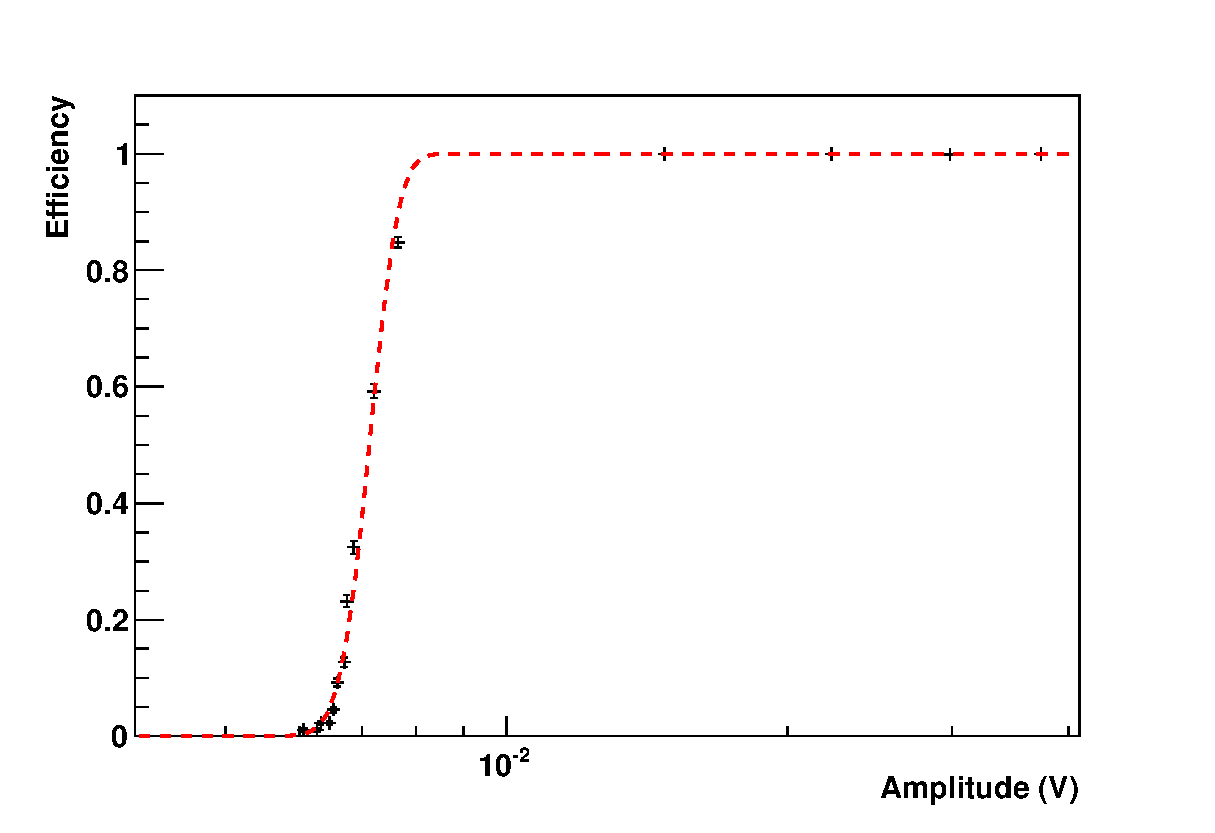
\includegraphics[width=0.9\textwidth]{energy_efficiency_bege}
				\caption[\bege~triggering efficiency measured with a pulser]
				{\bege~triggering efficiency measured with a pulser.  Error bars are binomial and the fit is to the error function in
				Equation~\ref{eqn:TrigEfficiency}.}
				\label{fig:BeGeTriggeringEfficiency}
			\end{figure}

		\subsection{Energy calibration}

Energy calibration at low energies is complicated by several factors.  In particular, low-energy x-ray peaks ($<10$~keV) from any source will be heavily attenuated by the source itself as well as materials between the source and the crystal, including the outer cryostat, mounting components, and the crystal dead layer.  Higher energy x-rays have a larger probability to interact in the crystal, but these are unsuitable for calibration because of their distance from the signal energy region which, in the case of dark matter, is close to threshold.  However, internal cosmogenic isotopes provide excellent candidates for calibration since there are several with characteristic lines near or below 11~keV.  Therefore, the energy calibration was determined by fitting the low-gain channel simultaneously to the peaks listed in Table~\ref{tab:XRayLines} yielding a linear equation:

			\[
			E_{ion} (keV) = a V + b
			\]  

with $a = 63.81\pm0.25$~(keV/V) and $b = -0.014551\pm0.016$~keV.  These results were applied to both the low- and low-gain channels.  An example of a typical fit spectrum is shown in Figure~\ref{fig:BeGeResFit} and in other figures throughout the remainder of the chapter.

		\subsection{Resolution of results}

The resolution of the detector was determined by measuring the intrinsic electronic noise using a pulser and by measuring the widths of x-ray lines.  These widths are measured by performing a simultaneous fit to prominent x-ray lines.  The fitting function is a combination of gaussians for each x-ray line, a flat background component, and a second `plateau' background component below the x-ray lines parameterized by an error function equivalent to Equation~\ref{eqn:InitialFitEqn} described earlier in Section~\ref{sec:BeGeSpecFit}.  The fit is shown in Figure~\ref{fig:BeGeResFit}.  
			\begin{figure}
				\centering
				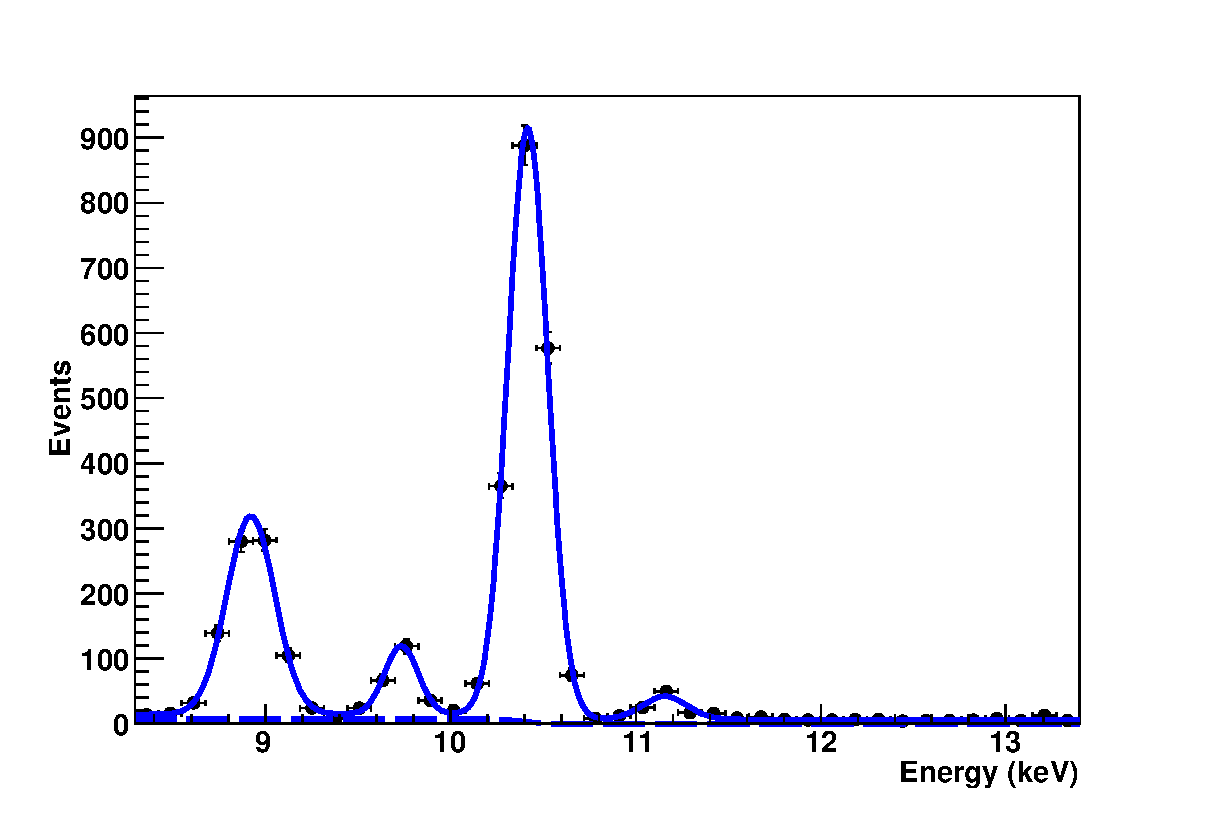
\includegraphics[width=0.8\textwidth]{FitResolutionPlot}
				\caption[Estimate of \bege~resolution]
				{Fit to estimate the resolution of the \bege, including gaussian fits to some of the prominent lines listed in Table~\ref{tab:XRayLines}.}
				\label{fig:BeGeResFit}
			\end{figure}
The results of these measurements were folded into the following equation:

			\begin{equation}
				\sigma = \sqrt{\sigma_{elec}^{2} + E \eta F}
				\label{eqn:SigmaEqn}
			\end{equation}

to determine the intrinsic electronic noise $\sigma_{elec}$ and estimate the Fano factor $F$.  $E$ is the energy in keV, $\eta$ the amount of energy required to generate an electron-hole pair (2.96 eV).  $\sigma_{elec}$ was found to be $70.48\pm0.54$~eV and $F$ was estimated as $0.241\pm0.013$.  Results are shown in Figure~\ref{fig:BeGeResPlot}.  As expected, the electronic noise measured with a pulser is independent of energy.  The scatter of the x-ray measurements is larger than statistically expected, in particular the \znsixfive~and \galsixeight~exhibit $\sigma$s well away from the best-fit line.  This is most likely due to insufficient bit depth of the digitizer and that this resolution is not properly included in the error bars\footnote{The resolution due to the bit depth of the digitizer (i.e.~keV/ADC count) should be small compared to the resolution of the measured process and so a future DAQ upgrade would benefit from such an improvement.}.  The low-gain channel has an intrinsic resolution of 1.95~mV/ADC, or $\sim125$~eV/ADC.  The actual resolution of the measurements estimating the amplitudes of pulses is better due to the fact that many samples are averaged together for that calculation.  However, the main purpose of this equation is to estimate the resolution of the x-ray lines at low-energy, around 1~keV, and it is clear that small deviations to this measurement do not significantly affect results in this region.

			\begin{figure}
				\centering
				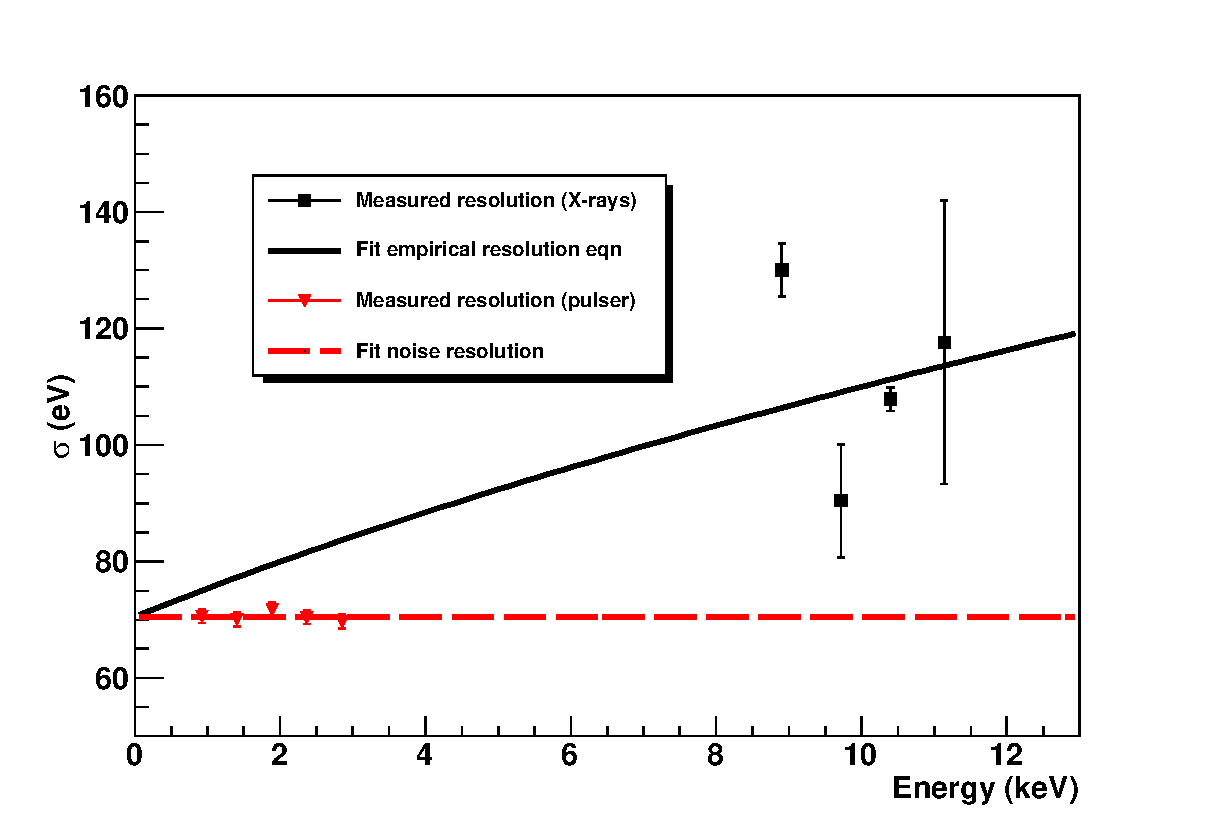
\includegraphics[width=0.8\textwidth]{resolution_plot}
				\caption[\bege~resolution versus energy]
				{\bege~resolution versus energy.  Red dashed line is measured and fit intrinsic electronic noise, 
				black points are measured resolution from x-ray lines, black line is a fit to Eqn.~\ref{eqn:SigmaEqn}.}
				\label{fig:BeGeResPlot}
			\end{figure}


%		\subsection{Baseline versus energy}
%		\label{sec:BeGeBaseline}

%Describe the baseline versus energy and the features we see in the data set.  Maybe not?


	\section{Data cleaning and cuts}
	\label{sec:BeGeCuts}	
	
	Several cuts were employed to clean the data, removing spurious events from electronics noise or microphonics.  Additionally, other cuts were employed to remove events with slow rise-time.  This section discusses the implementation and results of \emph{all} cuts performed on the data set.  
	
		\subsection{Microphonics and noise cuts}
	     	\label{sec:MicroCuts}	
	
	Vibrations in detector components at different electric potentials, such as the cryostat, cold-finger, or crystal mount, can induce electronic signals due to the changing capacitance created by the movement.  These electronic deviations can generate extra noise at low energies (threshold to a few keV) possibly obscuring any signals in that region.  During LN filling of the dewar, vibrations due to the filling generate a significant amount of additional microphonics noise from vibration caused by the influx of new liquid nitrogen.  See Figure~\ref{fig:BeGeLNExample} for an energy spectrum of events occurring during an LN fill.  
			\begin{figure}
				\centering
				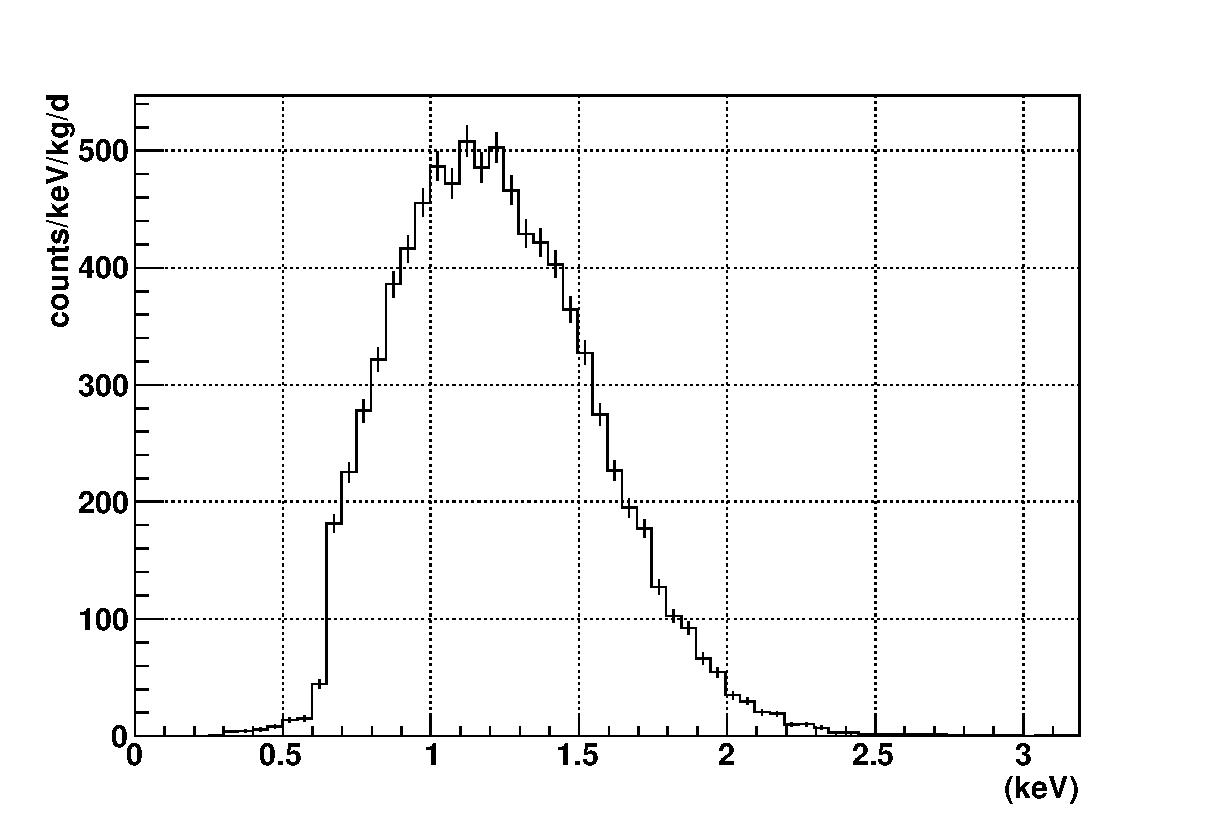
\includegraphics[width=0.8\textwidth]{LNFillEnergySpectrum}
				\caption[Energy spectrum during LN fills]
				{Energy spectrum during LN fills.  No microphonics cuts were applied to these data.}
				\label{fig:BeGeLNExample}
			\end{figure}
Therefore, during these filling periods, a flag was set in the data to enable later removal of events occurring during a fill.  This flag was then lowered 5~minutes after the fill completed, resulting in a veto time of $\sim$15~minutes.  LN fills occurred every 2 days, meaning that they occupied 0.5\% of the run time.  
		
	For microphonics induced from sources other than LN fills, another cut was
made.  Morales et al.~developed a technique to mitigate this class of events,
taking advantage of the fact that microphonics tend to have characteristics
(e.g.~rise-time, fall-time, baseline shift) significantly different from events
arising from charge collection in the crystal~\cite{Morales1992410}.  This
procedure analyzes the ratio of amplitudes from two signal channels with
different shaping times  and accepts or rejects events based upon their
deviation from the expected ratio.  This expectation can be determined by using
a source or a pulser at low amplitudes; in a setup where the amplification of
the two shaped channels is nearly equivalent, the expectation value of the ratio
is close to 1.  
	
	In this application, a pulser was used to train the microphonics cut by taking high-statistics pulser runs at several discrete amplitudes near the threshold.  At these discrete amplitudes, the ratios of the two channels were histogrammed and fit to a gaussian.  The cut points were then determined by taking the values $\mu \pm 3 \sigma$ to accept 99.7\% of the pulser events.  Since these cut points were estimated at discrete amplitudes, a 4th-order polynomial was fit to them to interpolate between the points.  The results of this are shown in Figure~\ref{fig:RatioOfShapedChannels}.  To avoid errors from the interpolation, the cut was softened forcing the upper limit to be greater than 1, and the lower limit to be no less than 0.8.  The final cut is then shown in Figure~\ref{fig:RatioOfShapedChannelsFinal} which shows an overlay of the calculated cut on data from a scanned pulser run (Figure~\ref{fig:RatioScannedPulser} and from the run data (Figure~\ref{fig:RatioData}).  Interesting to note is how the run data and the scanned pulser data follow a different distribution at energies above 1~keV, in particular that the scanned pulser data is centered around a ratio of 0.9 and the run data is centered at a lower value.  This suggests that the difference between a pulser and an actual crystal event become more significant at these energies: future calibrations should use a source instead of a pulser to ensure complete consistency.  Interestingly, it appears that there may exist a crescent-shaped distribution of events that runs through the low-energy acceptance region (beginning below threshold at high ratios and ending from $1\to2$~keV at low ratios).  Whether or not such a distribution really exists has not been determined, but will be considered as a possible background in this low-energy region.  

			\begin{figure}
				\centering
				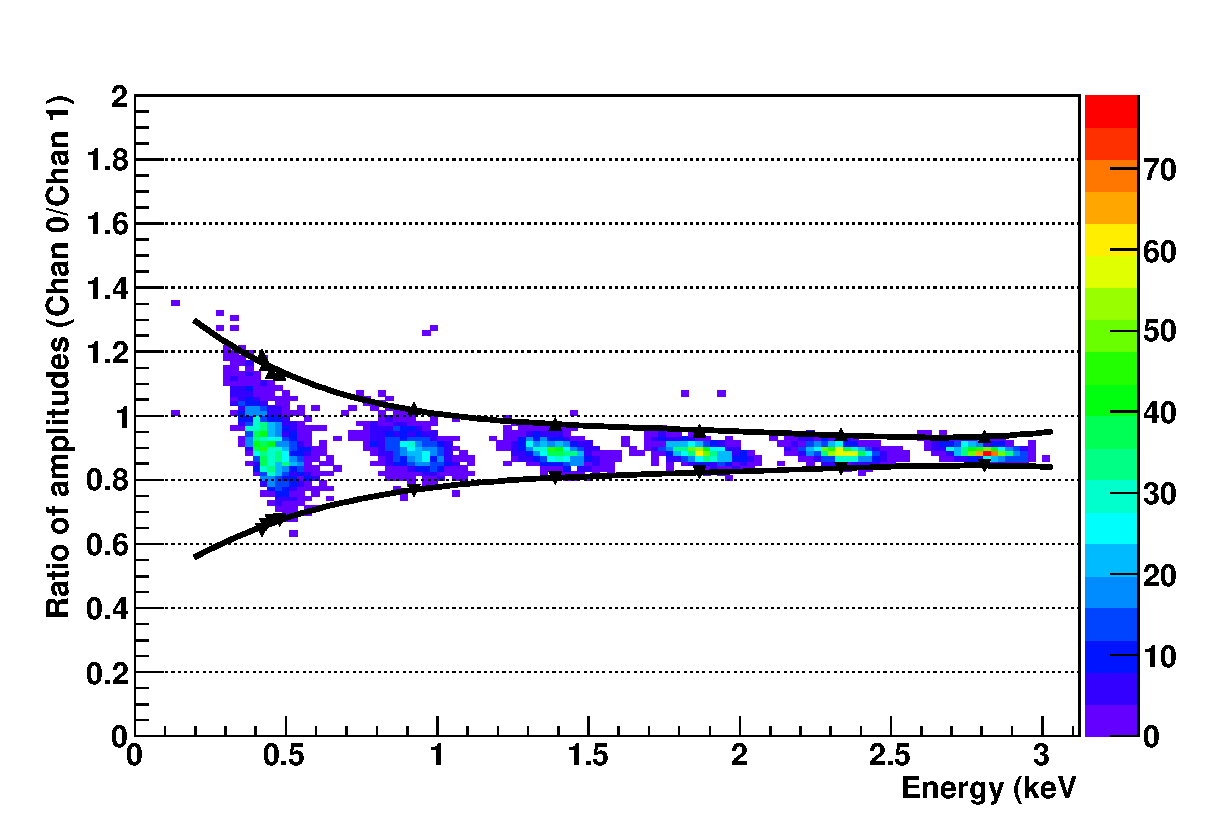
\includegraphics[width=0.8\textwidth]{Pulser_cut6}
				\caption[Calculation of microphonics cuts]
				{Calculation of microphonics cuts using the ratio of outputs from two different spectroscopy amplifiers with an 
				input pulser at discrete amplitudes.  Line is 
				an estimate of the cut, see text for details.  }
				\label{fig:RatioOfShapedChannels}
			\end{figure}

			\begin{figure}
				\centering
				\subfigure[Scanned pulser run]{
					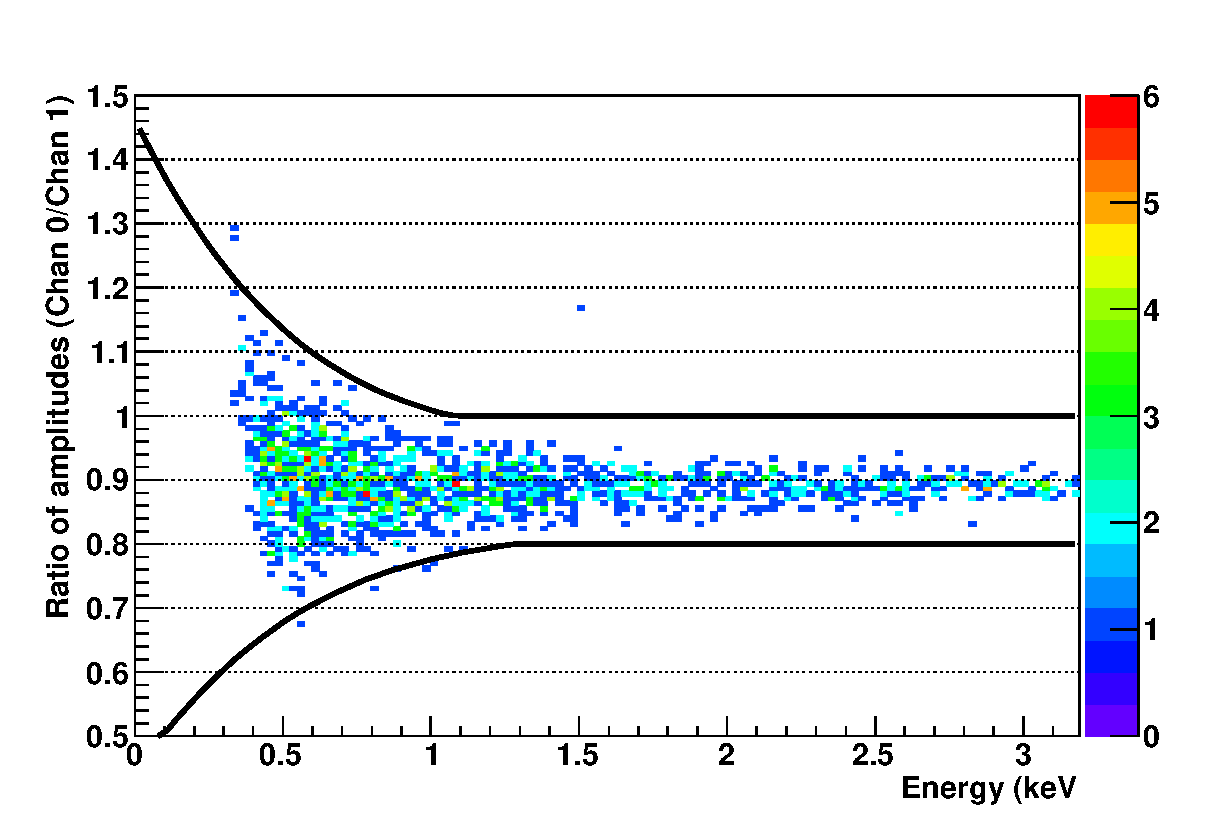
\includegraphics[width=0.46\textheight]{pulser_scan_with_cuts1}
					\label{fig:RatioScannedPulser}						
				}												
				\subfigure[Data]{
					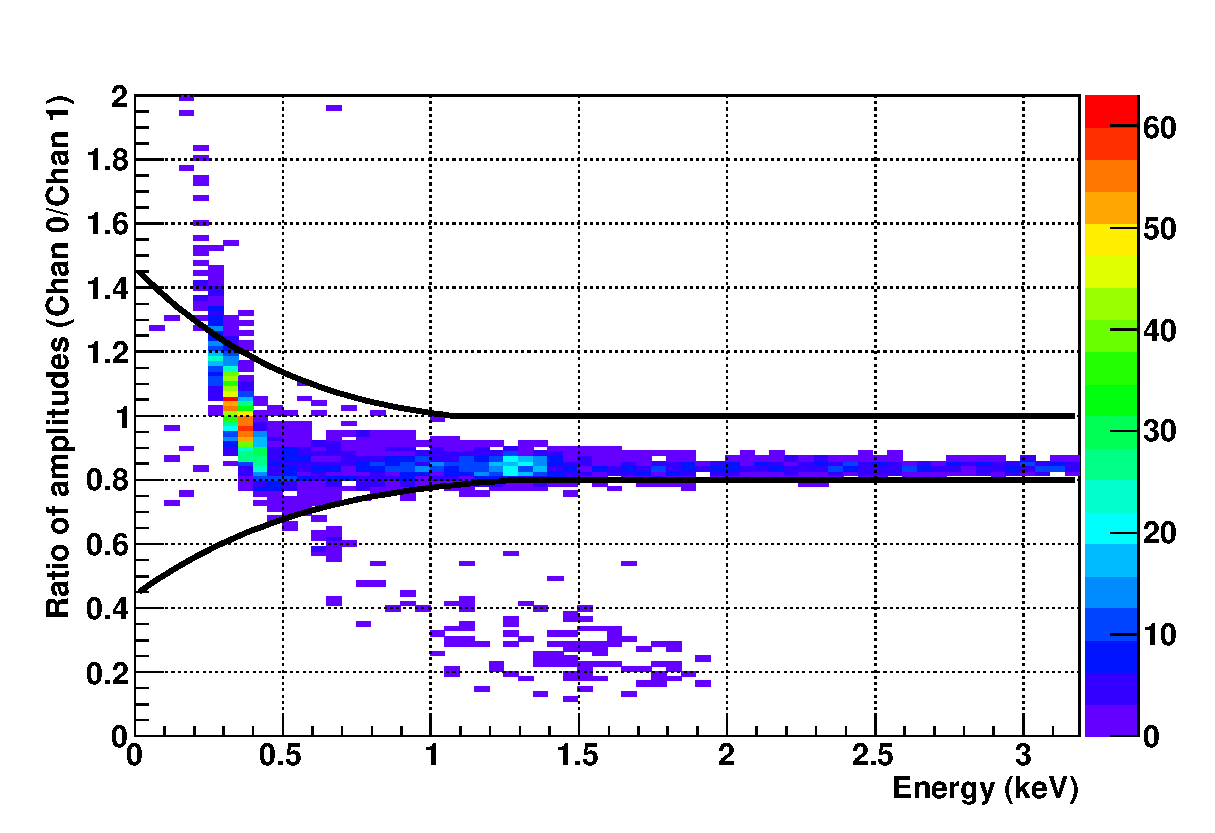
\includegraphics[width=0.46\textheight]{Ratio_of_amplitudes__Chan_0_Chan_1__vs_Energy__keV_}
					\label{fig:RatioData}						
				}				
				\caption[Microphonics cuts on data and scanned pulser runs]
				{Ratio of two shaped channels versus energy for a scanned pulser run and for run data.  The drawn line is the cut at 99.7\% efficiency, calculated using
				high-statistics pulser runs.}
				\label{fig:RatioOfShapedChannelsFinal}
			\end{figure}
	
	
		\subsection{Electronics cuts}
		\label{sec:BeGeElecCuts}
	
	This class of cuts was intended to remove events coming from spurious electronic events which were distinctly not signal events.  Only two electronics cuts were applied: the first to remove negative-going pulses including uncaught reset events that don't trigger the active veto, the second to remove noise pulses that were found to occur during a particular interval of the run time between 15 February 2010 and 15 March 2010.  
	
	The first cut removed events with a minimum in the shape channel below a certain voltage value chosen to be -0.02~V.  The population of events excluded by this cut included uncaught reset pulse events, negative-going events, and large energy depositions resulting in significant undershoot on the baseline.  Most of these events also saturated the digitizer positively, but many of the negative-going events did not.  A full explanation for these events was not determined though it is possible that some may arise from breakdowns of the crystal voltage.  From this cut, only 184 events were removed over the 150.375~day run period, generating a negligible reduction in live-time.
	
	While running tests analyzing the rates of events in different energy regions (see Section~\ref{sec:BeGeRate}), a class of events was found that occurred only during a sub-interval of the run time from 15 February 2010 until 15 March 2010.  These events were distinctive from true events, but were problematic because they populated the spectrum near threshold around 0.5~keV.   An example of such a pulse is given in Figure~\ref{fig:OddPulseExample}.  These were distinguishable by comparing the difference between the extrema (maximum - minimum) of the unshaped waveforms.  A plot of this parameter versus energy is given in Figure~\ref{fig:OddPulseCut} where the dashed line denotes the region of parameter space populated by these pulses.  
	
	To study the origin of the pulses, a rate analysis similar to that performed in Section~\ref{sec:BeGeRate} was applied to the subset of events.  The time between these events was histogrammed and fit to an exponential; the results are included in Figure~\ref{fig:OddPulseRate}.  This revealed that the events arrived not with a defined frequency, but rather in a Poisson fashion with a rate estimated from the fit as $2.97 \pm 0.1$ counts/hour.  This can be compared to the normal rate for this energy region $0.5\to1$~keV of $\sim0.124$ counts/hour (see Section~\ref{sec:BeGeRate}).  The structure of the pulse suggests an induced signal possibly coming from a noise source capacitively-coupled to the signal lines.  It is likely that these pulses arose from some cross-talk issues from a separate, independent DAQ system that was connected to the detector in parallel at the time since the removal of this parallel DAQ system corresponded exactly to when these pulses stopped occurring.  This class of events was entirely removed using the discriminating line in Figure~\ref{fig:OddPulseCut}.
	
	
			\begin{figure}
				\centering
				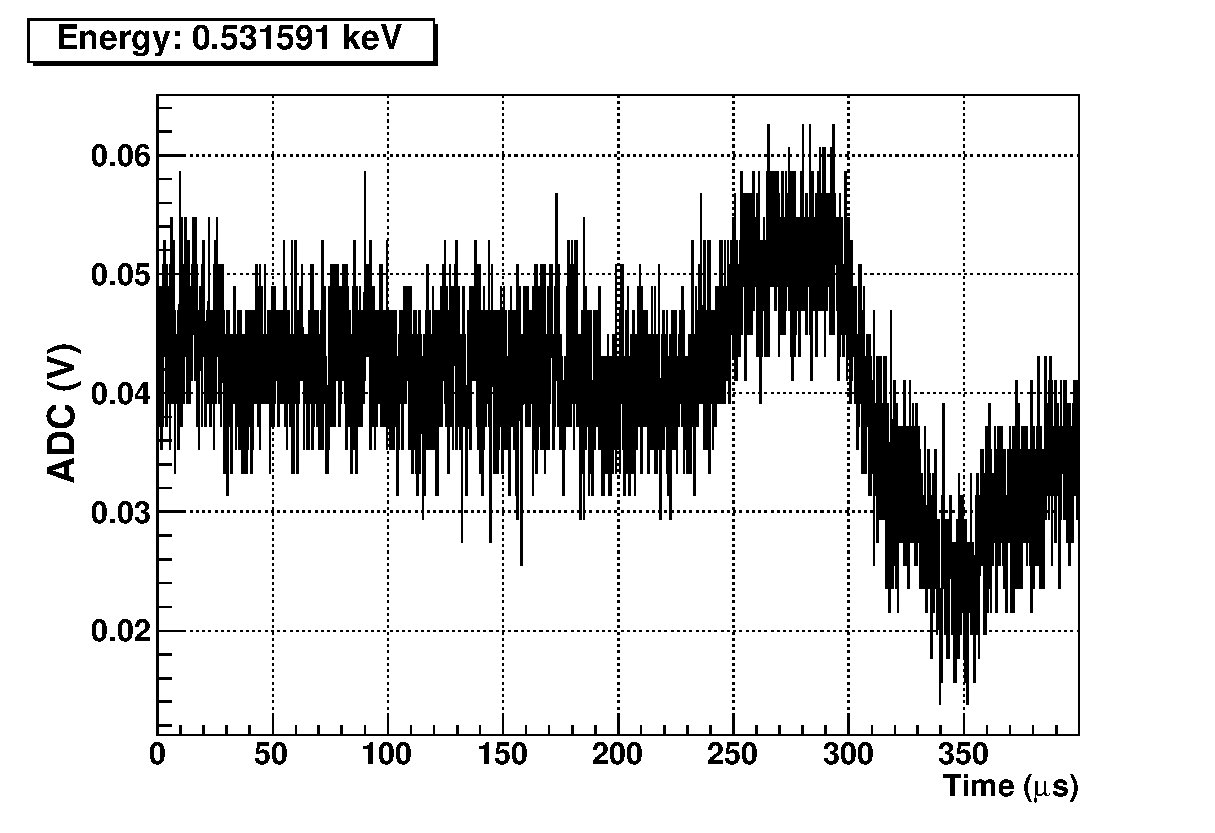
\includegraphics[width=0.8\textwidth]{ExampleOddPulse}
				\caption[Example of noise pulse of unknown origin]
				{Example of noise pulse of unknown origin.  The energy of the pulse is specified in the figure: 532~eV. 
				This indicates that these events can populate the spectrum near threshold.}
				\label{fig:OddPulseExample}
			\end{figure}	

			\begin{figure}
				\centering
				\def\plotwidth{0.76\textwidth}
				%\subfigure[All data] {
				%	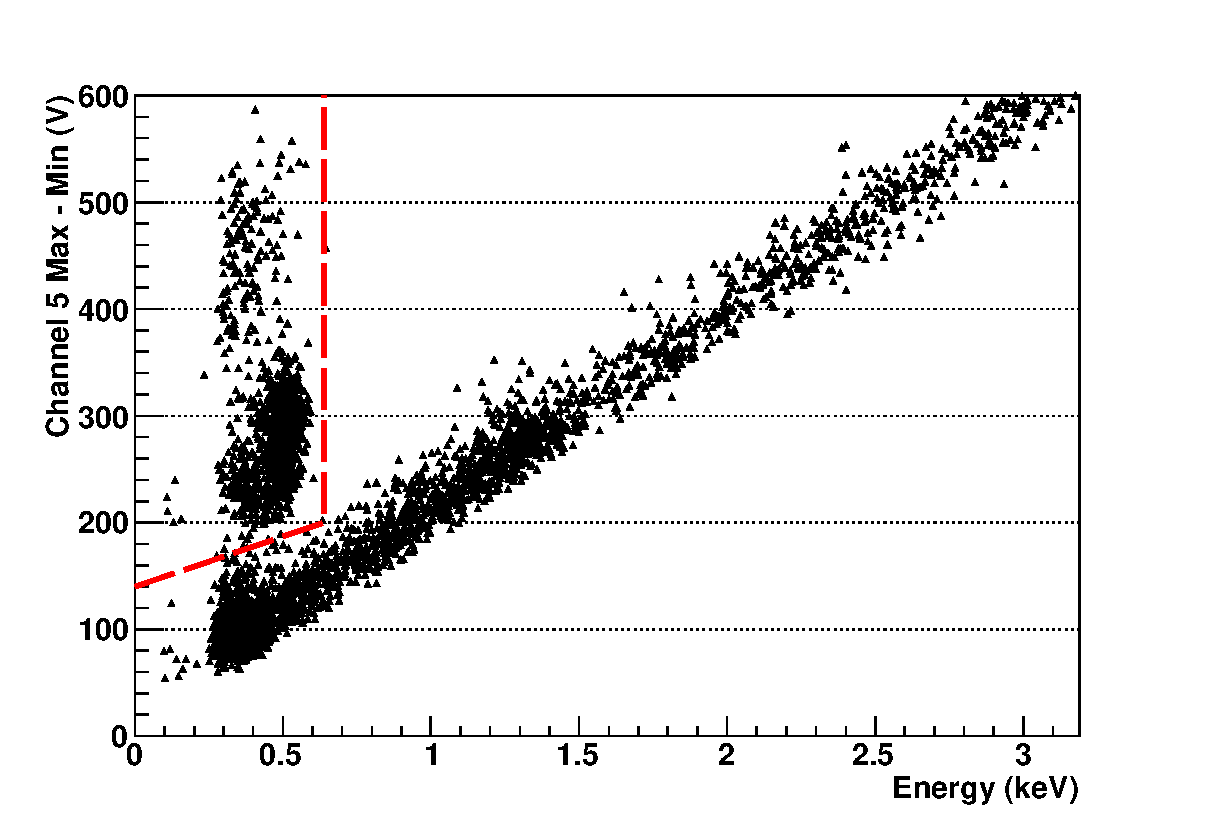
\includegraphics[width=\plotwidth]{Channel_5_Max_-_Min__V__vs_}
				%}
				\subfigure[Data around time of interest]{
					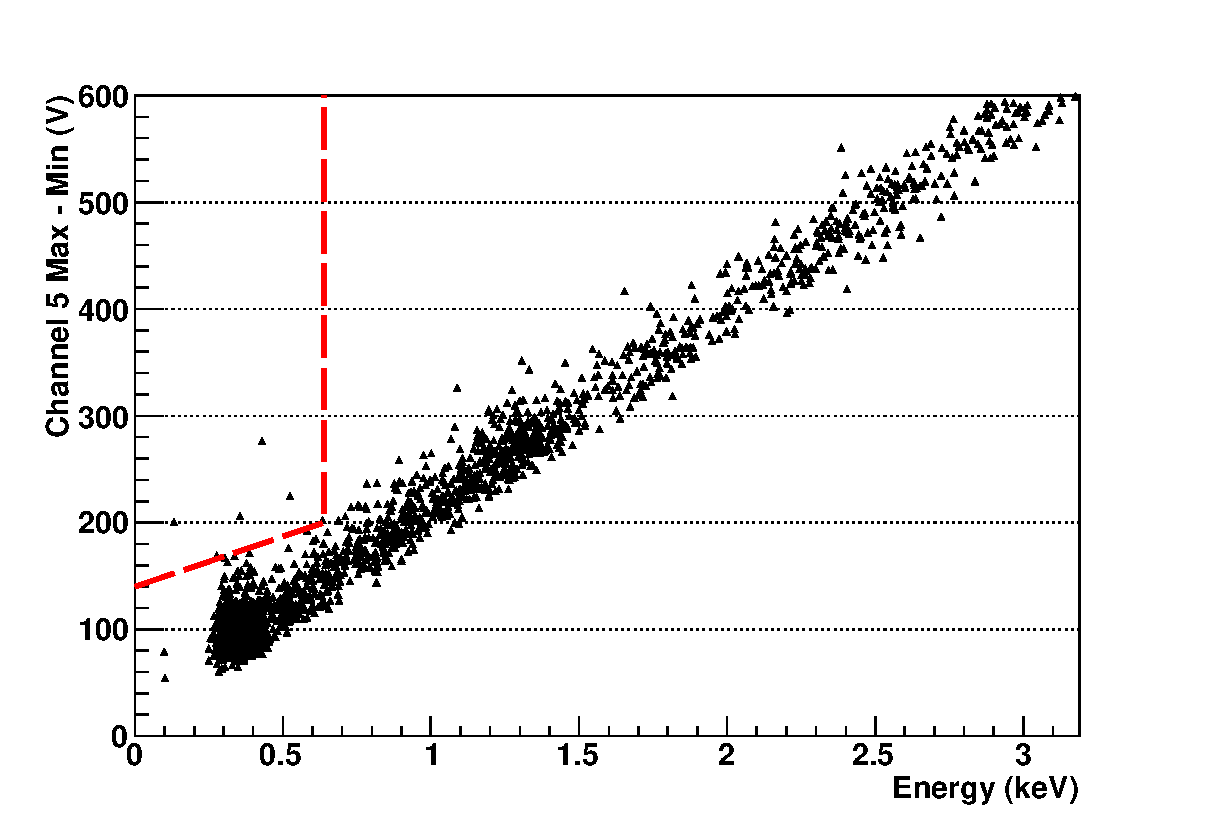
\includegraphics[width=\plotwidth]{Channel_5_Max_-_Min__V__vs_before}				
				}
				\subfigure[Data during time of interest]{
					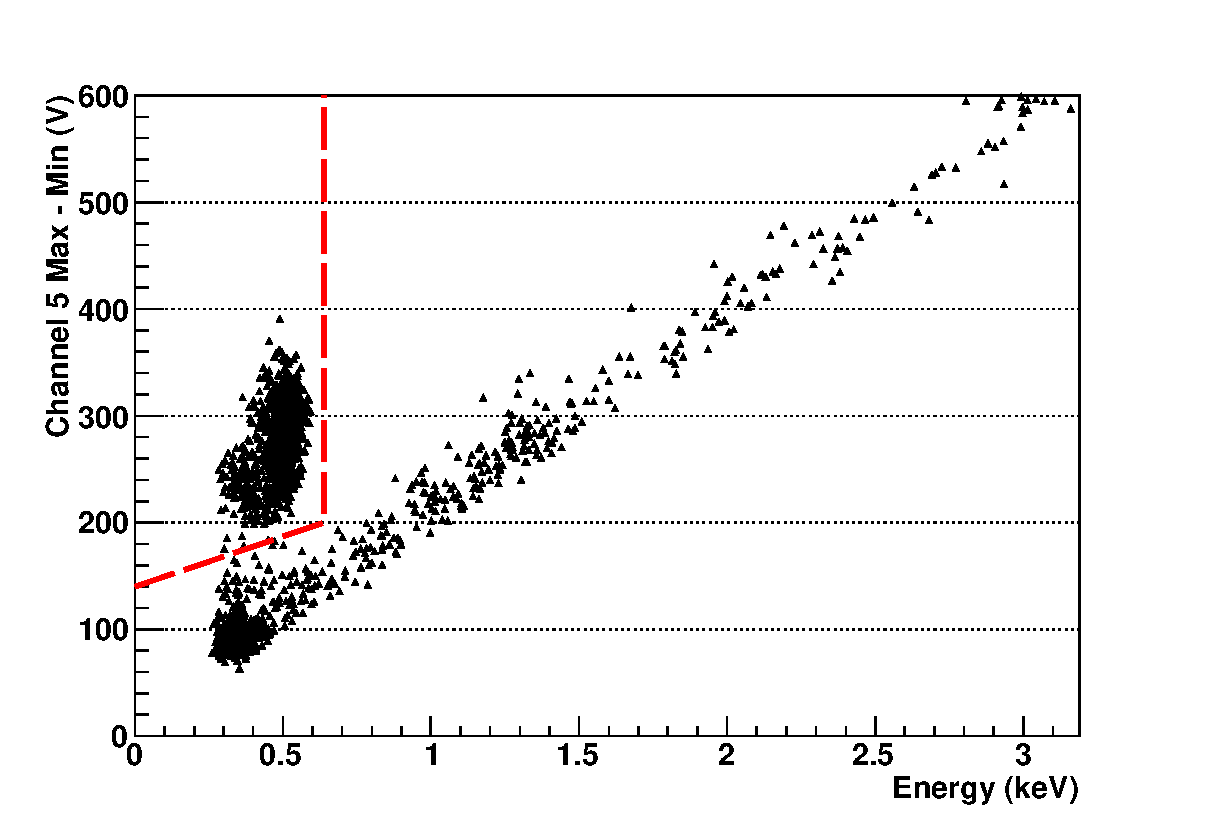
\includegraphics[width=\plotwidth]{Channel_5_Max_-_Min__V__vs_during}				
				}				
				\caption[Difference in unshaped waveform extrema versus energy]
				{Difference in unshaped waveform extrema (maximum - minimum) versus energy.  The dashed line is an indication of the cut used to exclude the 
				noise events removing all events within the selected region.  A plot of the data around the time of interest
				show that only $O(1)$ `true' events are removed by this cut.  }
				\label{fig:OddPulseCut}
			\end{figure}

			\begin{figure}
				\centering
				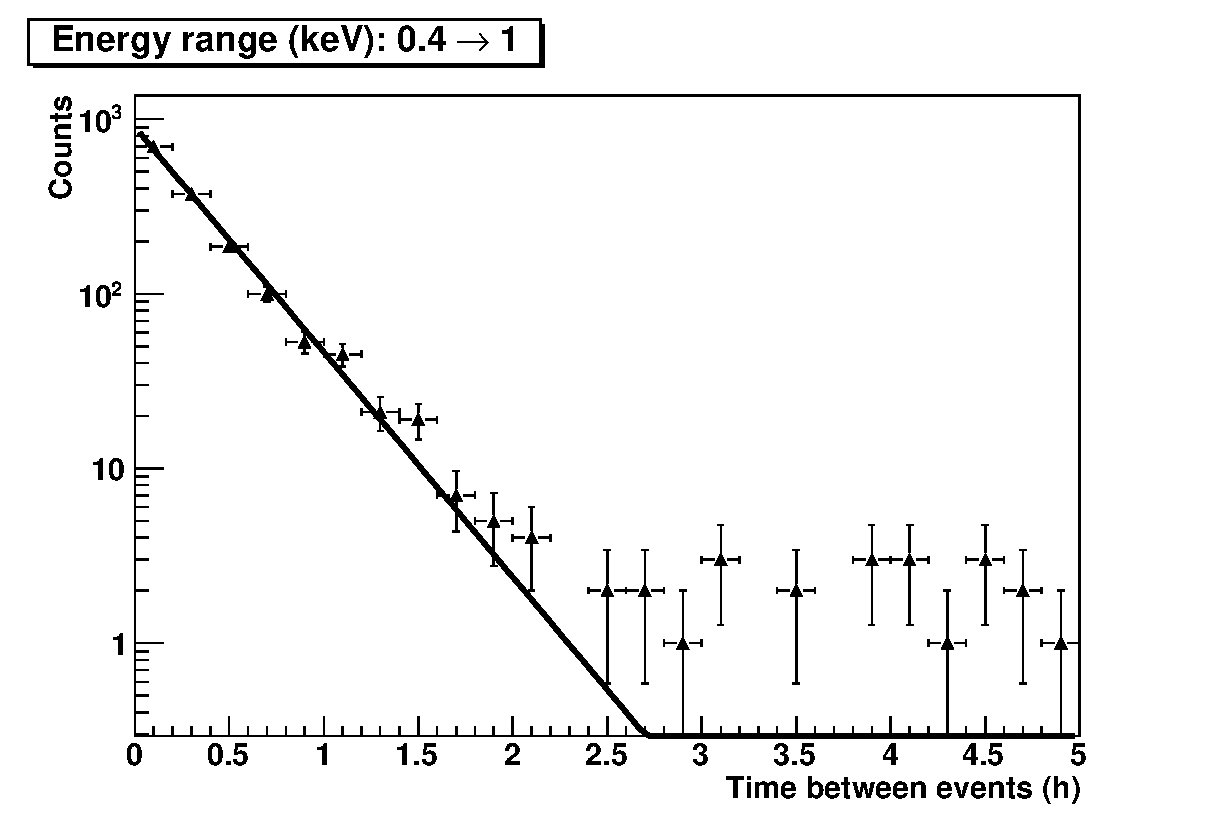
\includegraphics[width=0.8\textwidth]{odd_pulsesExponential_0.4_1}
				\caption[Time between noise pulses]
				{Time between events in the energy region $0.4\to1$~keV including noise pulses described in the text. 
				 The line is a fit to an exponential.  The events at longer time intervals are `contaminations' from non-noise
				 events arriving at a much slower rate.}
				\label{fig:OddPulseRate}
				%FixME: do analysis on only the bad pulses.
			\end{figure}
				
		\subsection{Rise-time cuts}
	     	\label{sec:RisetimeCuts}	

	Pulses of slow rise-time were found during the deployment of \ppc2 (see Section~\ref{sec:DeploymentPPC2SoudanAnalysisRisetime}).  These pulses were predominately at low energy near threshold which meant that they could compose a possible background to any signal in this region.  This section studies the methods developed to measure the rise-times at low signal-to-noise ratios against threshold and explores systematics related to a cut on this quantity.  Additionally, the likely origin of these pulses and possible tests for further exploration are discussed. 
	
			\subsubsection{Wavelet de-noising}
		     	\label{sec:RisetimeCutsWaveletDenoise}
					
	As the amplitude-to-noise ratio of waveforms shrinks at low energies, calculating the rise-time becomes more sensitive to the magnitude of the noise (i.e.~the electronic fluctuation of the signal) due to the reduction in signal-to-noise.   De-noising via a simple bandpass filter is undesirable when both signal and noise are distributed across similar frequency bands as the signal-to-noise ratio will not be enhanced by removing particular frequencies.  When calculating the rise-time of a pulse, a bandpass filter can greatly attenuate the high frequencies present in the rising edge of the pulse.  Wavelet shrinkage provides methodology to reduce noise on a generic function (see e.g.~\cite{Don95bb,Don95aa}) when the function and noise occupy the same frequency space.  The algorithm follows:
				\begin{enumerate}
					\item Choose a wavelet basis.
					\item Perform a wavelet transformation using the chosen basis to a level $n$, 
					obtaining $n$ sets of detail and approximation coefficients.
					\item Apply thresholding to the detail coefficients.
					\item Perform an inverse transformation.
				\end{enumerate}
	In this particular application it is necessary to use a translation-invariant version of the wavelet transformation called a Stationary Wavelet Transformation (SWT) (see~\cite{Coif95aa,Naso95aa}).  The SWT performs transformations at all possible translations for a given data set and basis wavelet.  A subsequent inverse SWT effectively averages these together, avoiding artifacts induced by any chosen time origin of the waveform.  Examples of artifacts induced by using a origin-dependent transformation instead can be found in~\cite{Coif95aa,Naso95aa}.
	
				\begin{figure}
					\centering
					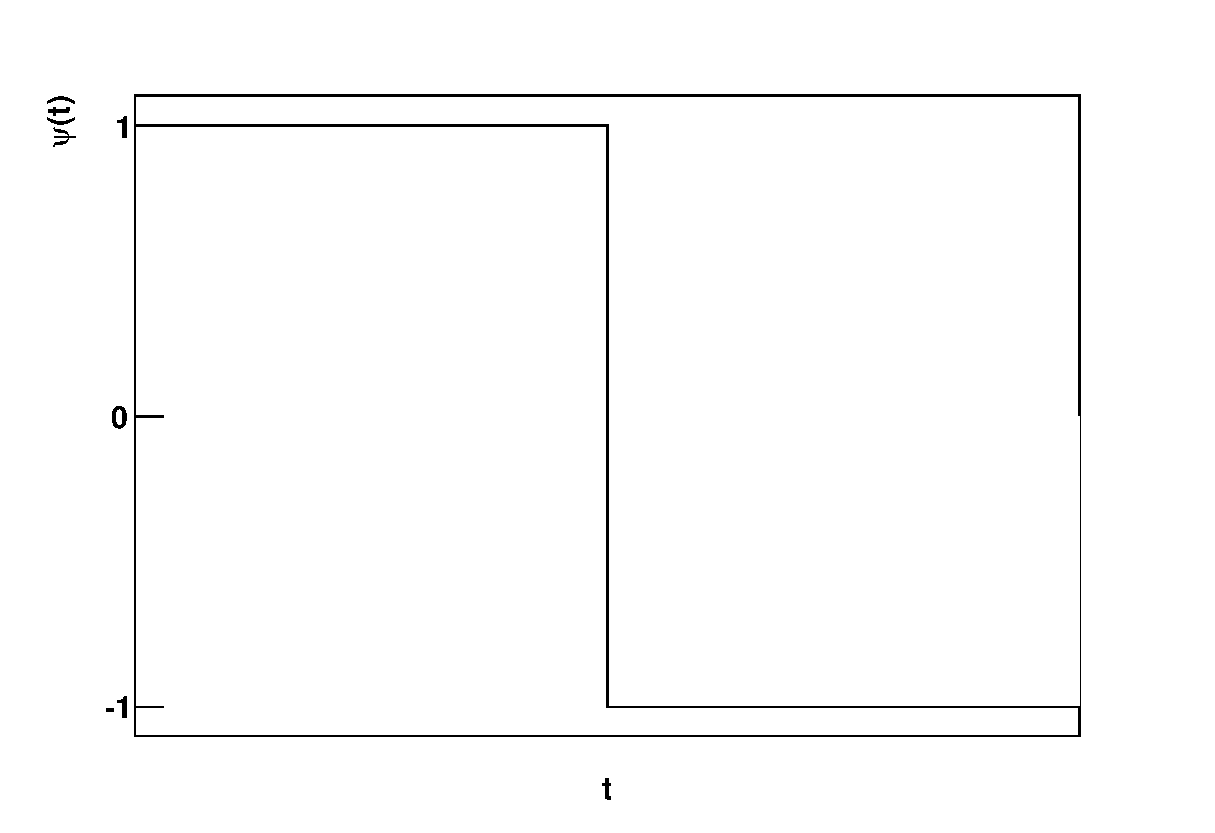
\includegraphics[width=0.95\textwidth]{HaarWavelet}
					\caption[Haar wavelet]
					{An example of a Haar wavelet.  This base wavelet may be scaled and translationally shifted
					to compose a complete basis set.}
					\label{fig:HaarWavelet}
				\end{figure}					


	For this wavelet analysis, the python package PyWavelets~\cite{PyWave} was
used.  Since an implementation of the inverse SWT was missing from this
distribution, the necessary extension to the package was written (see
Section~\ref{sec:WaveformProcMGDO}).  A Haar wavelet (see Figure~\ref{fig:HaarWavelet}) was chosen as a basis
wavelet due to its simplicity and asymmetry.  In this case, the asymmetry of
the wavelet is desirable because the signal (an unshaped preamplifier trace)
exhibits the same characteristic.  Thresholds for each set of detail
coefficients, $D_{n}^{(i)}$, were calculated using a pure-noise waveform
training set of length $j$.  For each noise waveform $x^{(i)}$, a 6-level SWT
was used to generate $D_{n}^{(i)}$ and the thresholds were calculated for each
level $n$ according to the equation proposed by Donoho and
Johnston~\cite{Don95ad}:
	
				\begin{equation}			
					\tau_{n}^{(i)} = \sigma_{n}^{(i)} \sqrt{2 \log N^{(i)}}
				\end{equation}			
				\[
					\sigma_{n}^{(i)} = \frac{\operatorname{MAD}\left(D_{n}^{(i)}\right)}{0.6745}
				\]
with $N^{(i)}$ the length of waveform, $x^{(i)}$, and MAD is the median average deviation.  The threshold at a level $n$ was then defined as $\tau_{n} = 0.8 \max(\tau_{n}^{(0)},...,\tau_{n}^{(j)})$.  An example of the coefficients calculated using a 6-level SWT is shown in Figure~\ref{fig:RisetimeCutsWaveletDecompositionOfPulse}.  This figure also includes the thresholds calculated at each level, denoted by dashed lines.  

Noise reduction was implemented by applying hard thresholding to each set of detail coefficients.  In this technique, all coefficients $D_{n}$ with an absolute value less than the threshold $\tau_{n}$ were set to zero.  Coefficients above this threshold value were unchanged.  The resultant coefficients were then used in an inverse SWT to produce a de-noised waveform.  An example of the wavelet de-noising is shown in the top figure of Figure~\ref{fig:RisetimeCutsExampleOfPulse}.
	
			
				\begin{figure}
					\centering
					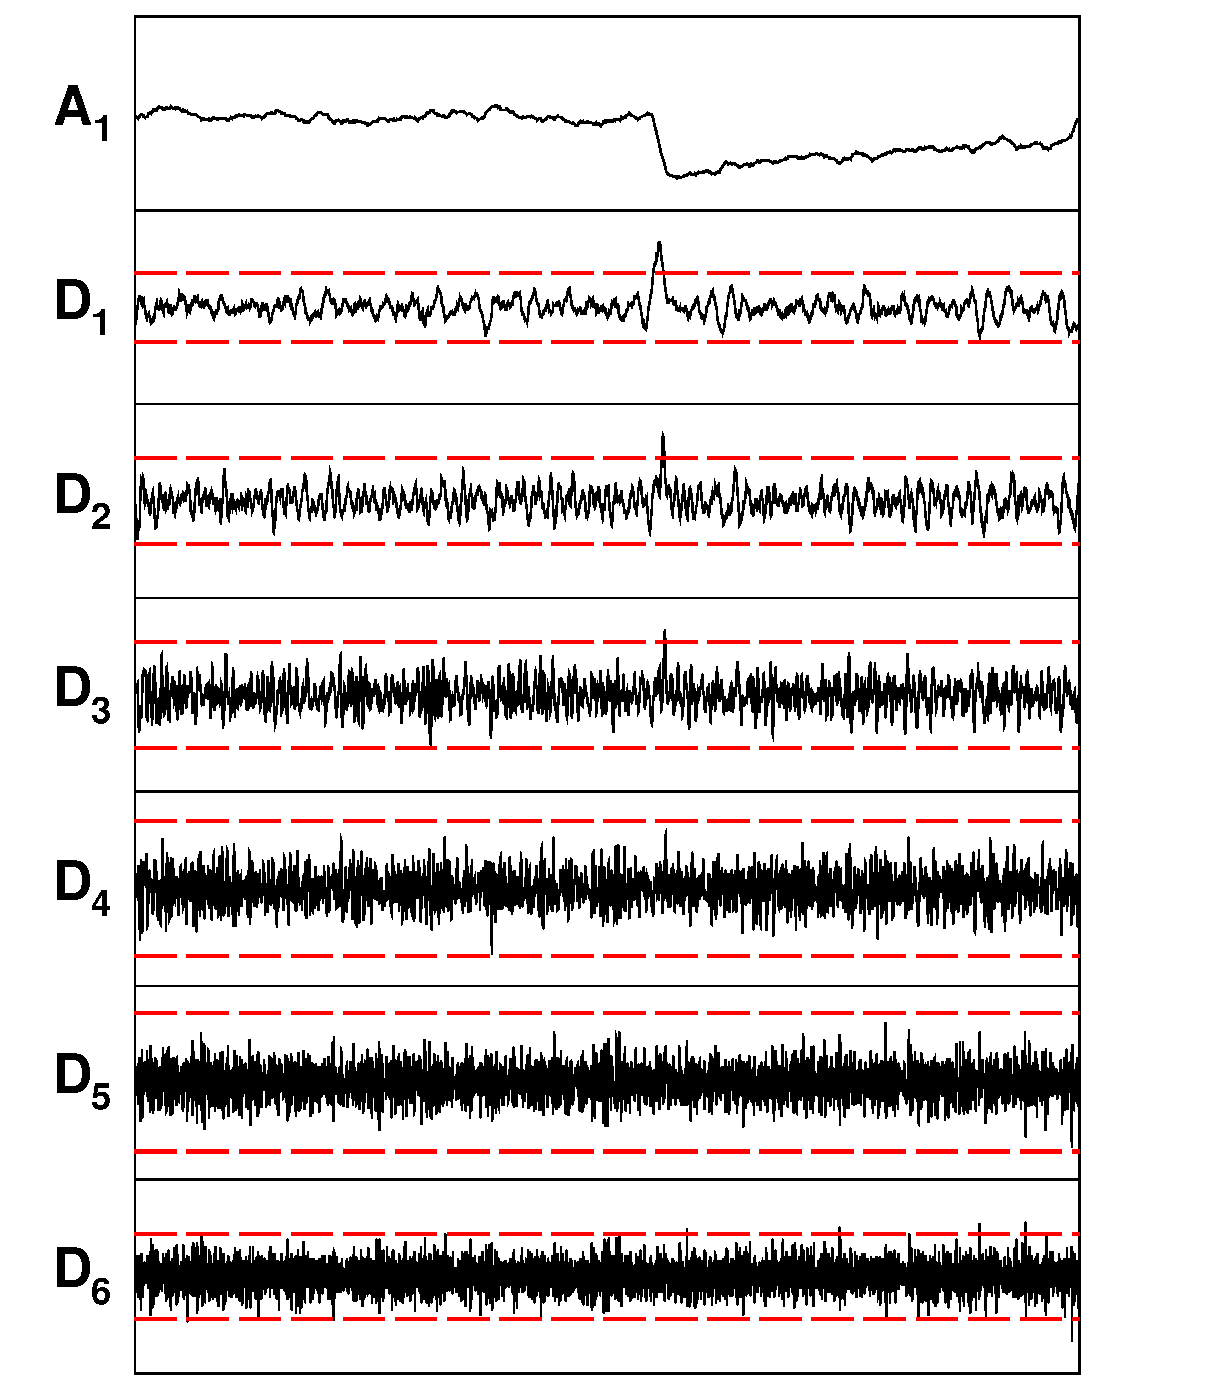
\includegraphics[width=0.95\textwidth]{ExampleWavelet}
					\caption[Example wavelet decomposition of pulse]
					{Example wavelet decomposition of pulse in Figure~\ref{fig:RisetimeCutsExampleOfPulse}.  
					A$_{1}$ denotes the first-level
					 approximation coefficients, the D$_{n}$ denote the detail coefficients at the $n$th level of the 6-level stationary wavelet 
					 transformation.  Dashed lines indicate the thresholding to be used for each set of detail coefficients.}
					\label{fig:RisetimeCutsWaveletDecompositionOfPulse}
				\end{figure}					

			\subsubsection{Rise-time calculation}
			\label{sec:RisetimeCalculation}
	The de-noising process ensured that the waveforms be ready for rise-time calculations.  After de-noising, the smoothed derivative of the waveform was generated using a Savitzky-Golay derivative filter~\cite{Sav64aa}.  The extremum of the derivative - in this case the minimum since the pulse was negative-going - was then found and used to determine the middle of the rising edge, $p_{m}$.  The full-width at half maximum (FWHM) was calculated and used to estimate the beginning and end of the rise of the waveform: the beginning, $p_{b} = p_{m} - 1.5\times$FWHM and the end, $p_{e} = p_{m} + 1.5\times$FWHM.  The baseline and amplitude of the pulse were each found by averaging over 1~$\mu$s (20~samples) beginning at $p_{b} - (1~\mu$s) and $p_{e}$, respectively.  These values were used to estimate the amount of time it took the pulse to rise 10\%$\to$90\% in amplitude.  Linear interpolation was used to refine the time values which came between digitization points.  An example of this calculation, employing the same pulse used to generate the wavelet decomposition in Figure~\ref{fig:RisetimeCutsWaveletDecompositionOfPulse}, is shown in Figure~\ref{fig:RisetimeCutsExampleOfPulse}.  
		
				\begin{figure}
					\centering
					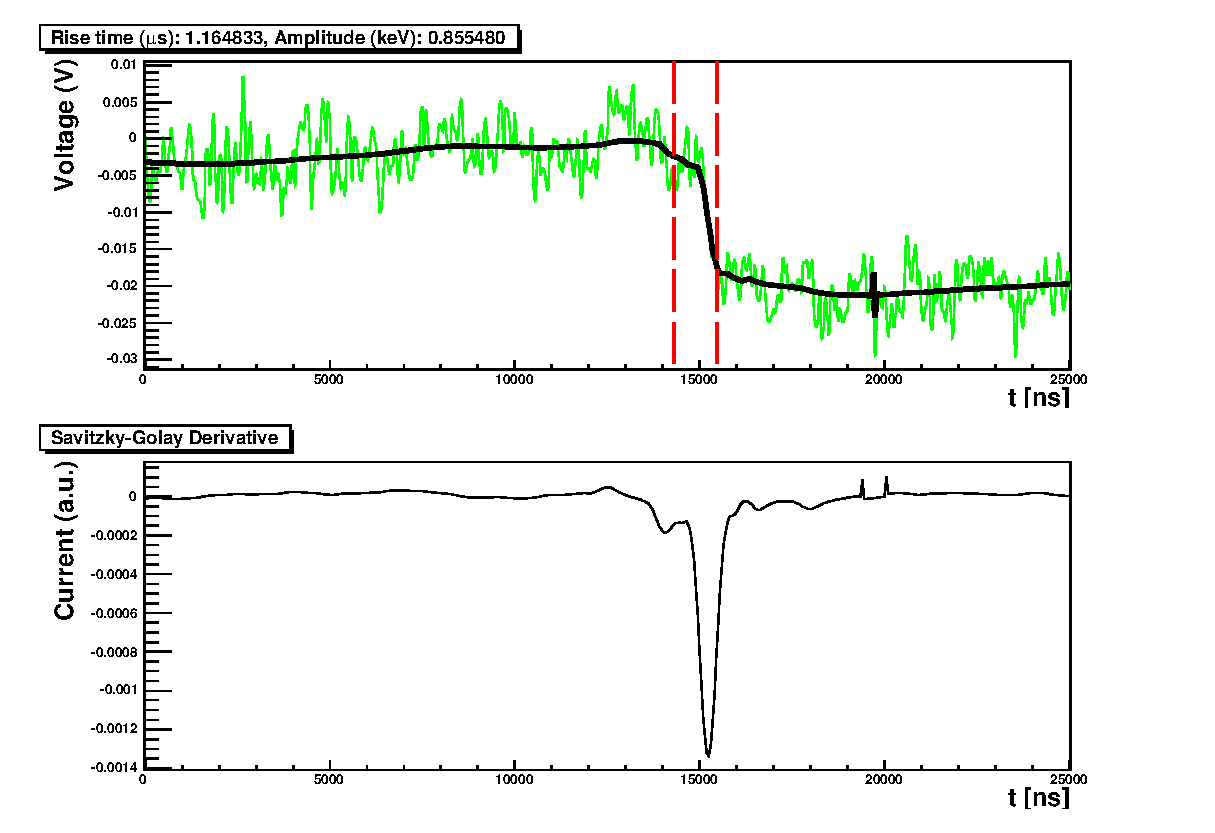
\includegraphics[width=0.9\textwidth]{ExampleWaveform0}
					\caption[Example of rise-time calculation technique applied to a preamp trace]
					{Example of rise-time calculation technique applied to a preamp trace.  
					The top shows the raw (green) and de-noised waveforms (black), and the vertical dashed lines represent the result 
					of the rise-time calculation.  The bottom plot shows the smoothed derivative of the trace calculated 
					using a Savitzky-Golay filter~\cite{Sav64aa} of degree~2, width~6.}
					\label{fig:RisetimeCutsExampleOfPulse}
				\end{figure}					

			\subsubsection{Rise-time simulation}
			\label{sec:RisetimeSimulation}
	
	To investigate how a cut based upon rise-time affected the spectrum, it was necessary to perform a simulation of the rise-time calculation on waveforms similar to the data.  The idea was to produce waveforms with similar characteristics (i.e. rise-time, noise) as seen in the detector and run them through the same algorithm used to analyze the detector data.  The waveform was generated by taking a tail pulse of 0~rise-time and running it through a digital low-pass RC filter.  The RC constant in the filter was tuned to reproduce the rise-time of ``fast'' pulses seen in the data.  In general this would not precisely reproduce all the characteristics of the detected pulses, but since the only parameter of interest was the rise-time it was reasonable to choose such a simple pulse construction.  An example of a simulated pulse before noise was added is given in Figure~\ref{fig:SimWaveformExample}
%Later systematic tests (Section~\ref{sec:RisetimeSystematicTests}) verified that it was sufficient.  
				\begin{figure}
					\centering
					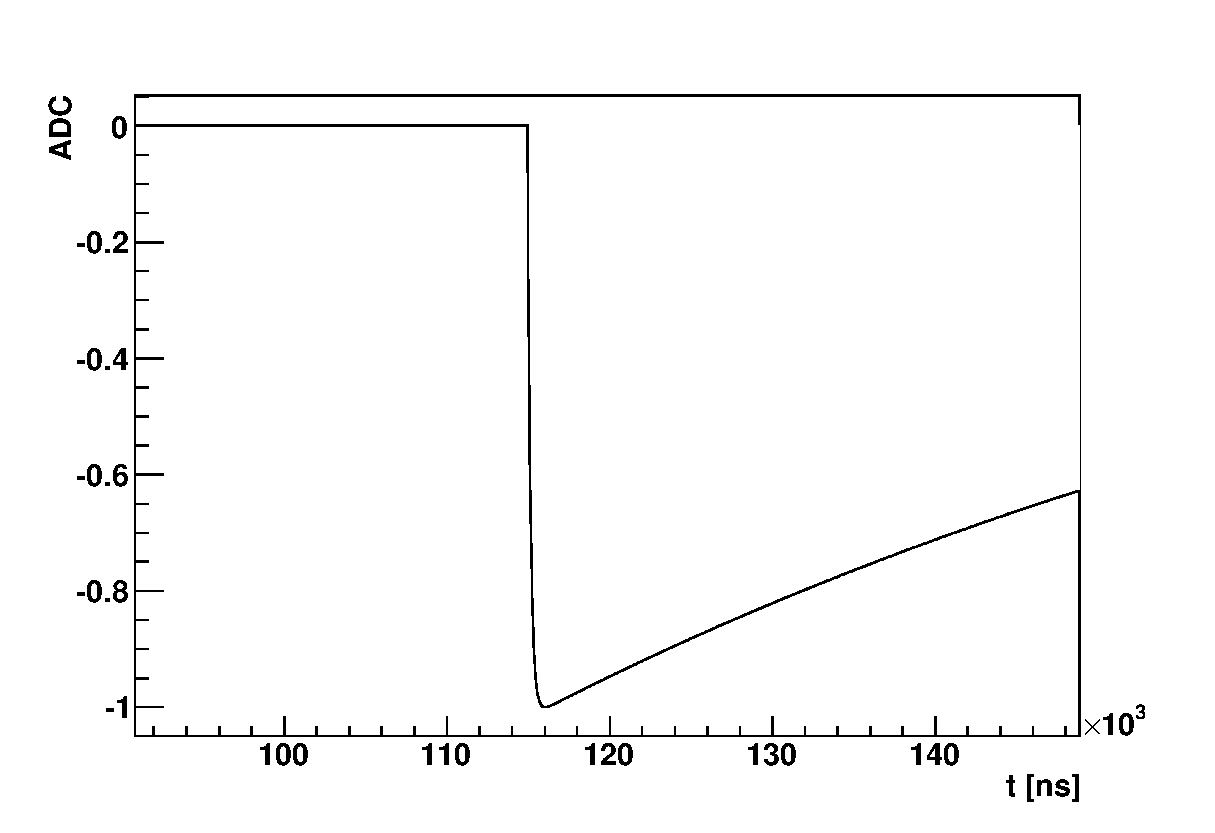
\includegraphics[width=0.9\textwidth]{SimWaveformExample}
					\caption[Example of a simulated pulse before the addition of noise]
					{Example of a simulated pulse before the addition of noise.}
					\label{fig:SimWaveformExample}
				\end{figure}
	
	The electronic noise of the detector was measured by looking at the baseline of all pulses and taking the average of power spectra for each preamp trace channel.  Once the average power spectrum was determined, it was possible to use this to add noise to the simulated pulse through the techniques outlined in~\cite{WanThesis08} by Wan Chan Tseung.  Essentially, a measurement of an average power spectrum, $\Omega = X^{2} + Y^{2}$ where $X$ and $Y$ are the real and imaginary components of the Fourier Transform, gives you an average value $\mu_{i}$ at a frequency bin $i$.  If there is no phase information in the noise (i.e.~$\tan^{-1} (X_{i}/Y_{i})$ is flatly distributed), $X_{i}$ and $Y_{i}$ are gaussian-distributed variables around 0 with the same standard deviation, $\sigma_{i}$, which is related to the average value of bin $i$ via  $\mu_{i} = 2 \sigma_{i}^{2}$.  Therefore, for each simulated pulse, a noise waveform was generated in frequency space, transformed to the time domain using a discrete inverse Fourier Transform, and added to the original simulated pulse.  
	
	Since the energy of each event was determined using the amplitude of shaped pulses, it was necessary to determine a relationship between amplitudes of the shaped and unshaped low-gain channels (channel 2 and channel 5) and the amplitudes of the shaped and unshaped high-gain channels (channel 1 and channel 4).  This was done by fitting the relationship from data, an example of which is shown in Figure~\ref{fig:Risetimechan2vschan4}.  Additionally, the waveforms' position in the trace window exhibited a dependence on the energy of the event: for events of smaller amplitude the trigger tended to arrive later, so that the waveform moved left in the trace window.  This dependence was measured by tracking the start of the pulse in the trace window versus amplitude and fitting it to an empirical polynomial (see Figure~\ref{fig:TriggerPositionDependence}).  This information was folded back into the simulation to control the starting point of the pulse given its amplitude.
	
					\begin{figure}
						\centering
						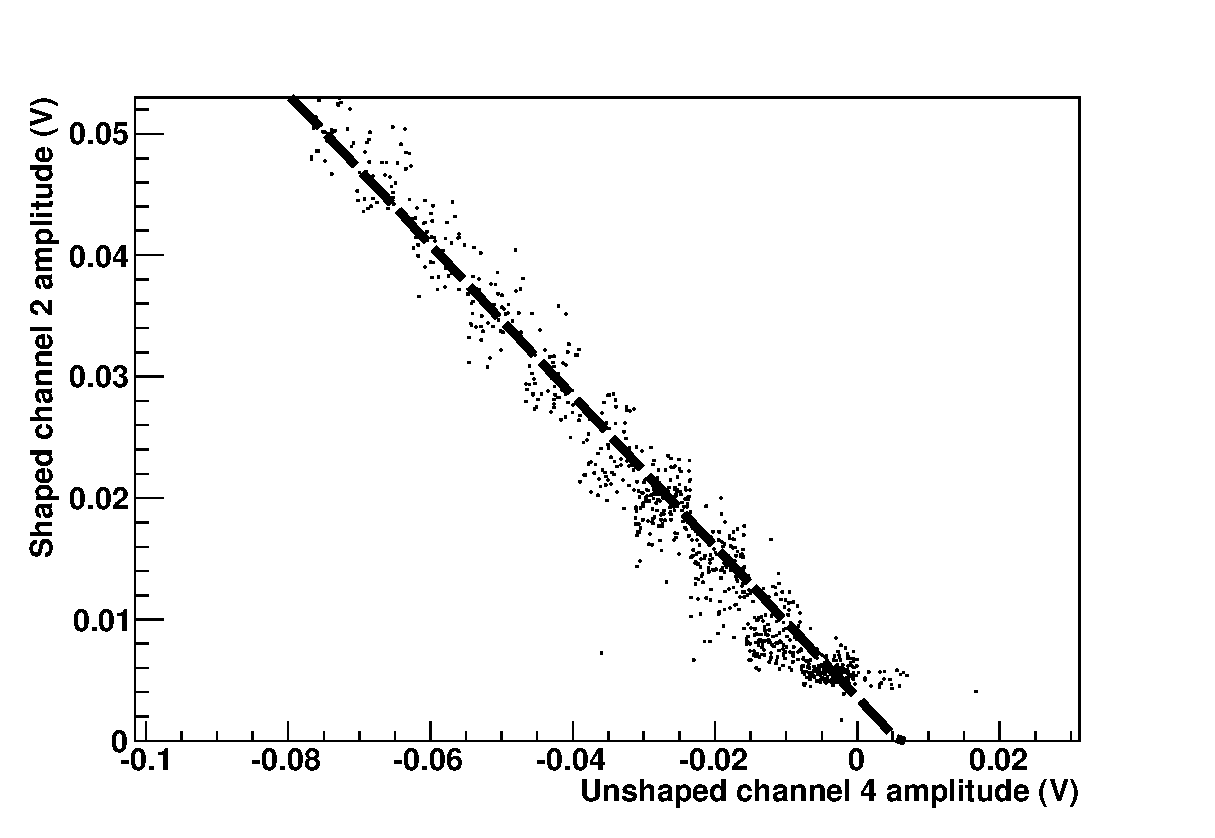
\includegraphics[width=0.9\textwidth]{chan4amplitude_vs_chan1}
						\caption[Unshaped amplitudes vs.~shaped amplitudes in the \bege]
						{Comparison between the amplitudes in the unshaped channel 4 and shaped channel 1.  											The line is a linear fit to the data.  The spectroscopy amplifier
						output positive-going pulses whereas the preamplifier output negative-going pulses which explains why the slope 
						is negative.  The voltage ranges on both the x and y axis have been made large enough to include events from the
						entire energy range.}
						\label{fig:Risetimechan2vschan4}.
					\end{figure}
					
					\begin{figure}
						\centering
						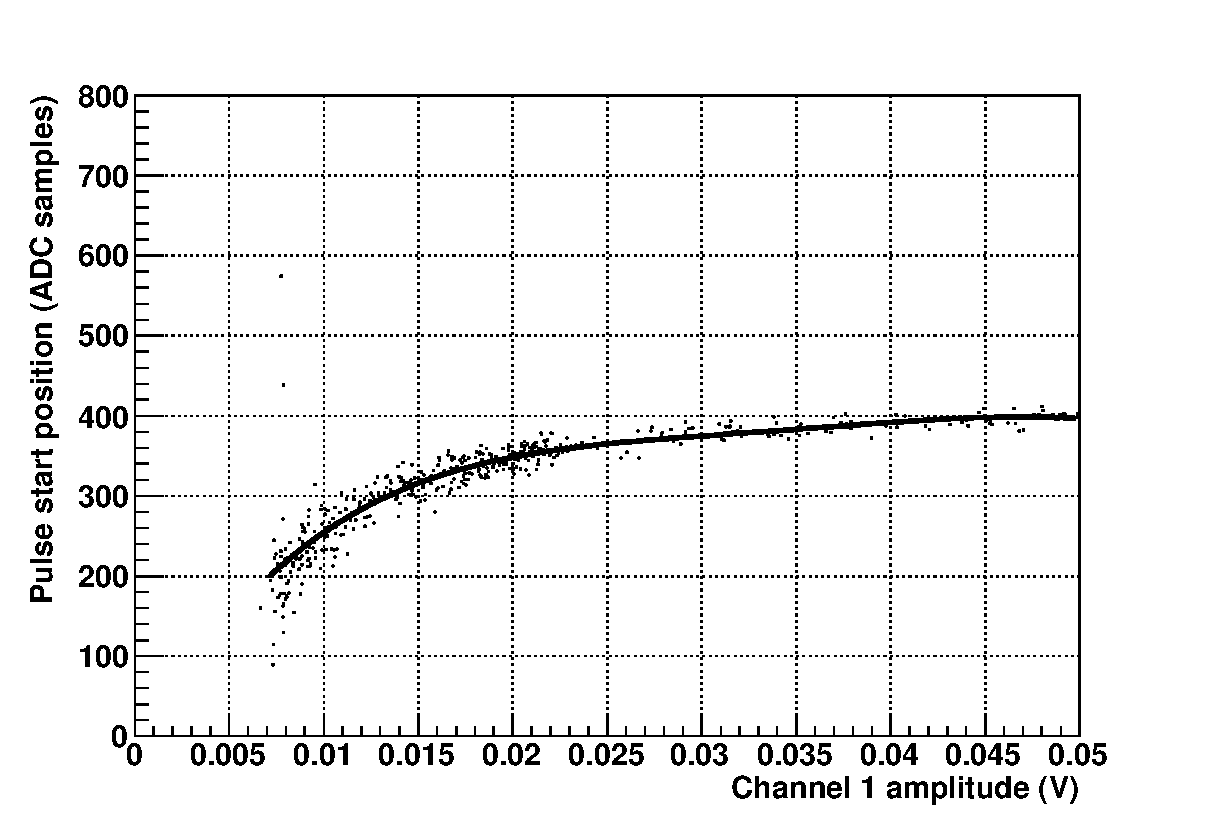
\includegraphics[width=0.9\textwidth]{start_pulse_vs_energy}
						\caption[Start of the preamp pulse versus the amplitude of the shaped channel]
						{Comparison between the start of the preamp pulse rise-time and the amplitude of the shaped
						 channel.  The line is a fourth-order polynomial fit which is used to parameterize this relationship, the order
						 of the polynomial was chosen `by eye'.}
						\label{fig:TriggerPositionDependence}.
					\end{figure}					
	
	Once the simulated pulses were generated, they were run through the same analysis chain as the waveforms from the detector, in particular through the rise-time calculation algorithms described earlier in this section.  The amplitudes of the pulses were sampled according to the triggering efficiency measured in Section~\ref{sec:BeGeTrigEff}.  Two simulations were run, one for each the high- and low-gain set of channels, for $\sim$5M events.  These results were then used to calculate contours of particular acceptances, 20, 30, 40, 50, 60, 70, 80, 90, 95, and 99\%.  To calculate the contour, the data were binned in a 2-dimensional histogram with energy bin sizes for the low- and high-gain channels, respectively, 1.6~eV and 0.4~eV, and time bin sizes of 5~ns.  Slices of the histogram were then taken at each energy bin and the upper limit of time calculated which accepted the required percentage of events.  Results of the simulation for the low-gain channel are shown in Figure~\ref{fig:RisetimeSimulation} along with a calculated 99\% acceptance contour.  The acceptance region is defined as all waveforms having a calculated rise-time less than or equal to the calculated contour.  A comparison of the calculated line to data for both high- and low-gain channels appears in Figure~\ref{fig:RisetimeDataVsCut}.  The acceptance lines shown in both of these plots exhibit an increase as the energy nears threshold due to the reduction of the signal-to-noise making it more difficult to reliably extract the true rise-time.
					
				\begin{figure}
					\centering
					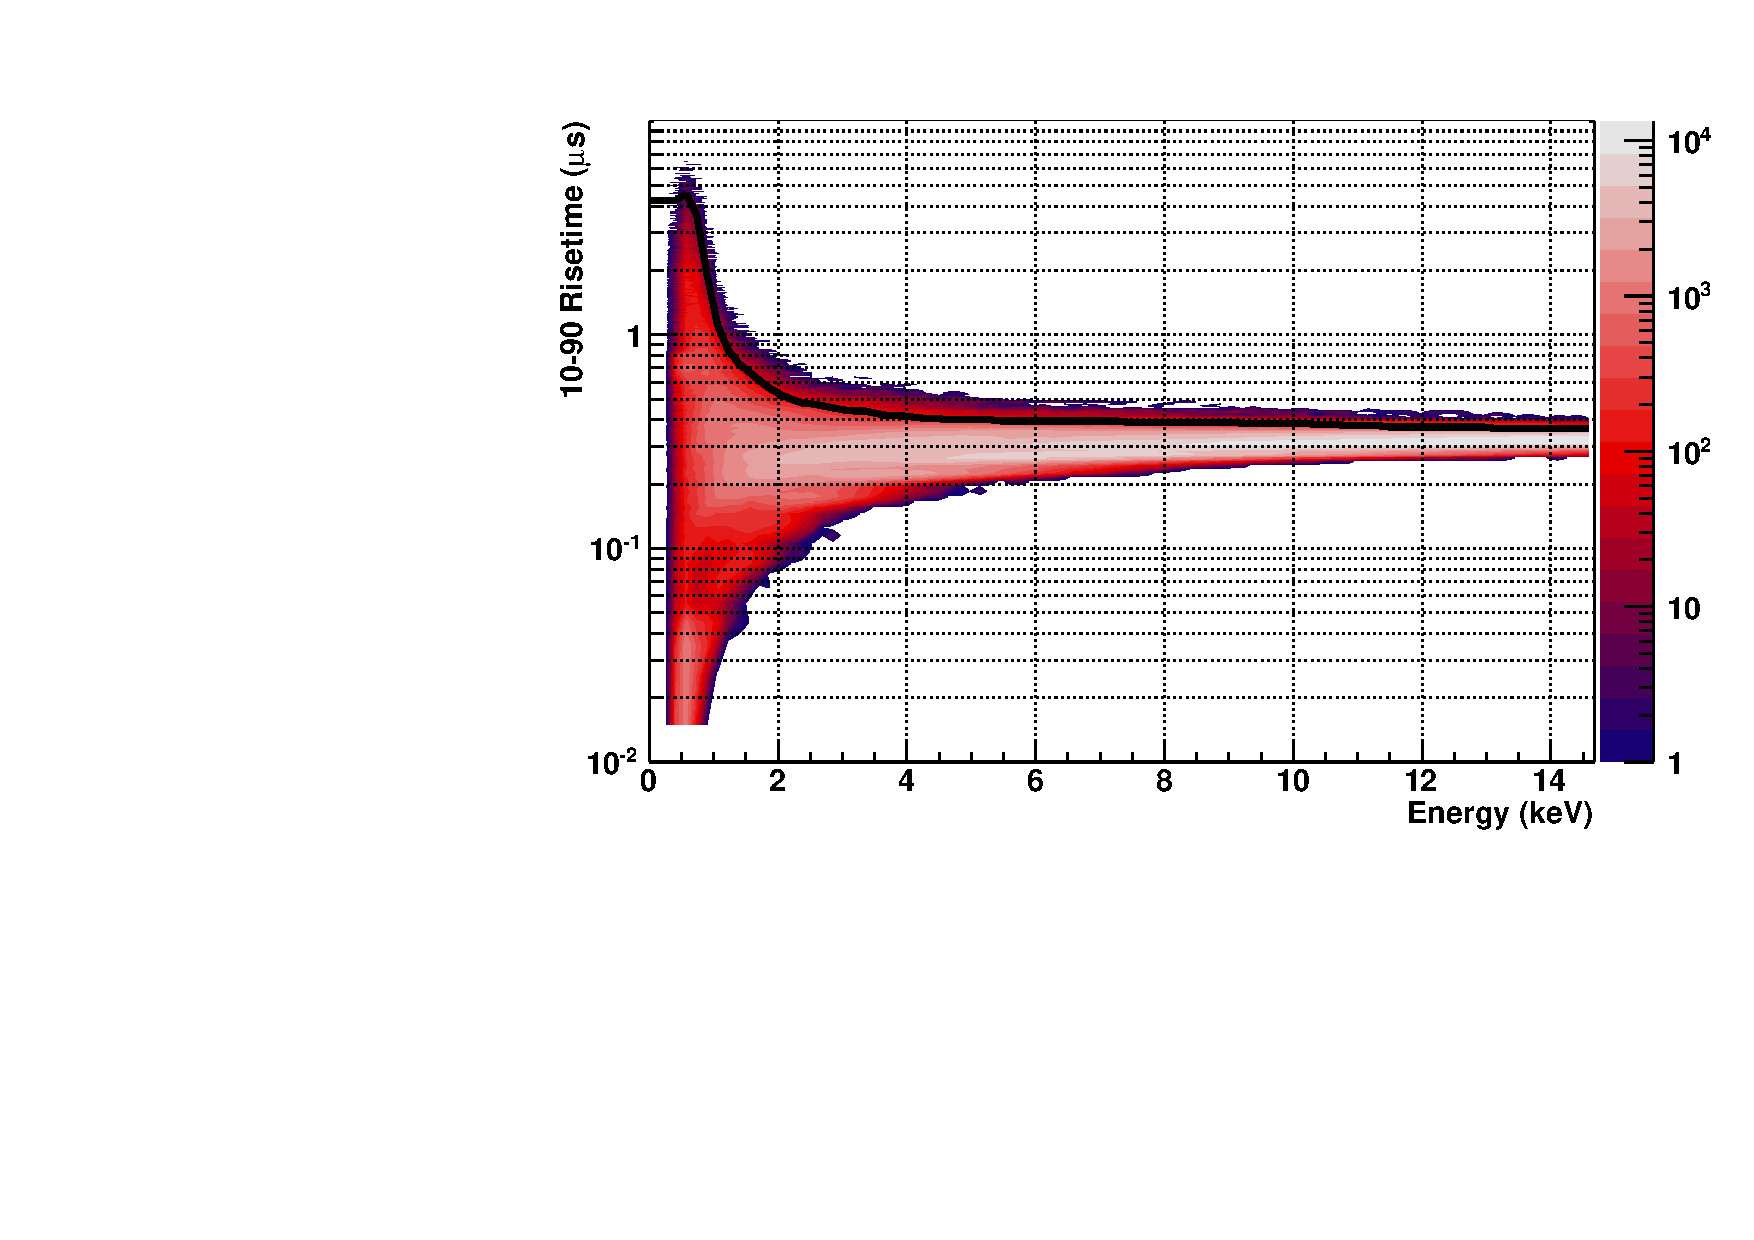
\includegraphics[width=0.9\textwidth]{risetime_cut_chan5_nice}
					\caption[Simulation of calculated rise-time for the low-gain channel of the \bege]
					{Simulation of calculated rise-time for the low-gain channel of the \bege.  
					The line is the calculated 99\% contour, which includes 99\% of events below the line.}
					\label{fig:RisetimeSimulation}
				\end{figure}	
	
				\begin{figure}
					\centering
					\def\plotwidth{0.8\textwidth}					
					\subfigure[High-gain channel] {
						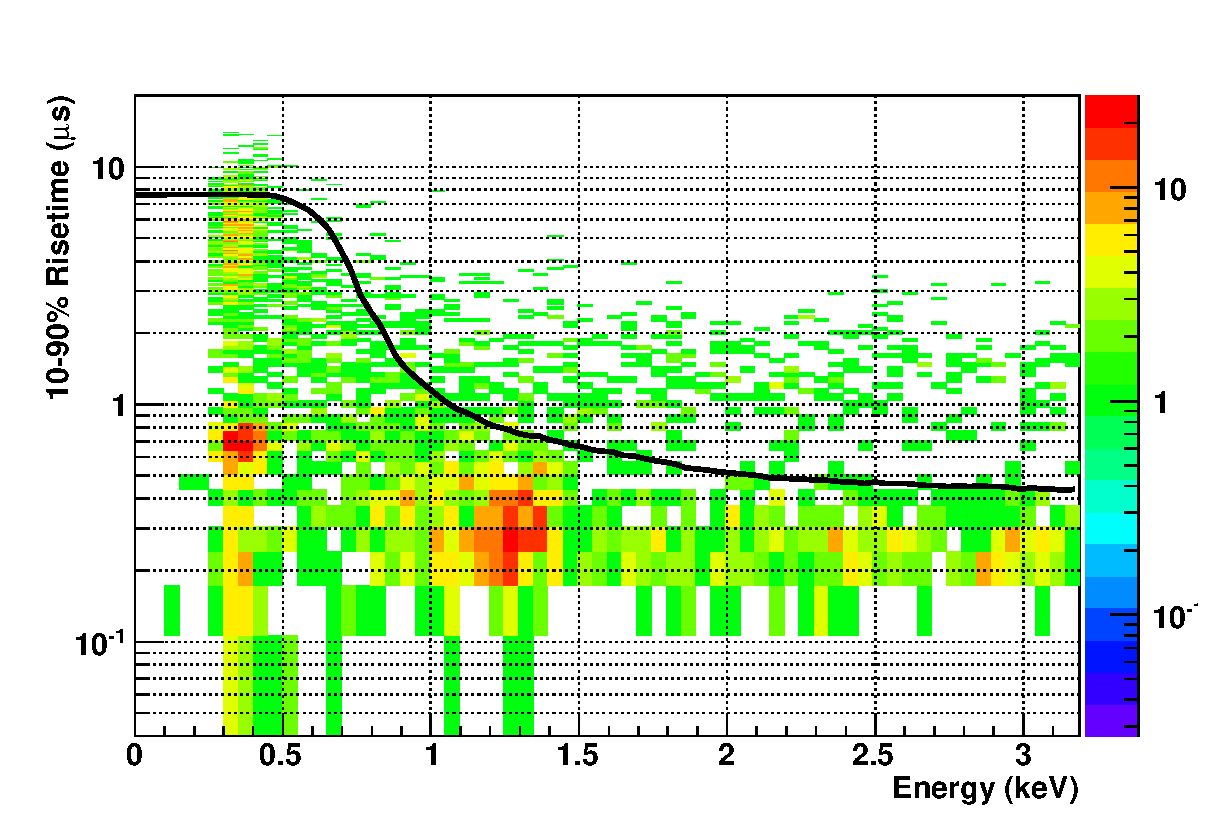
\includegraphics[width=\plotwidth]{lowrisetime}
						\label{fig:RisetimeDataVsCutHighGain}
					}
					\subfigure[Low-gain channel] {
						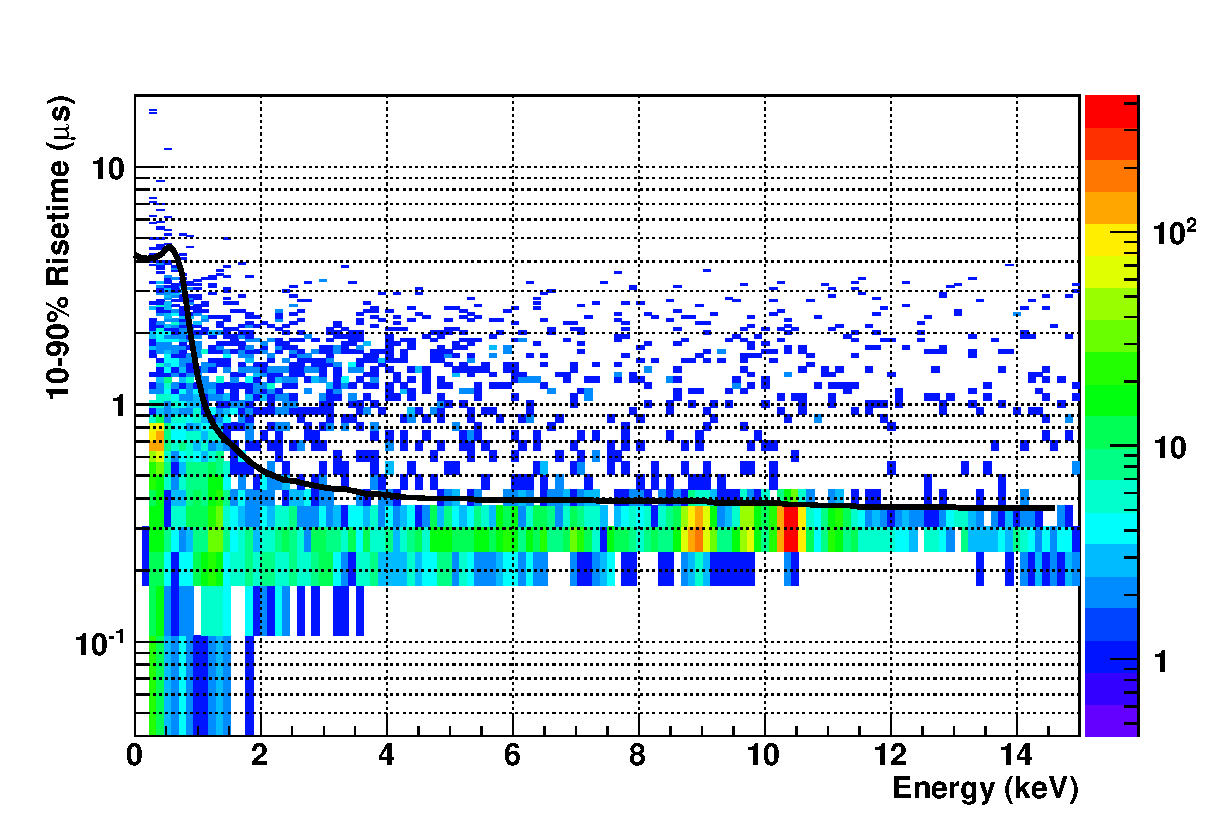
\includegraphics[width=\plotwidth]{highrisetime}
						\label{fig:RisetimeDataVsCutLowGain}						
					}
					\caption[Measured rise-time vs.~energy with a calculated rise-time cut of 99\% acceptance]
					{Measured rise-time versus energy.  The line is a calculated rise-time cut of 99\% acceptance, 
					removing events that fall above the line.}
					\label{fig:RisetimeDataVsCut}
				\end{figure}	
	
		\subsubsection{Rise-time systematic tests}
		\label{sec:RisetimeSystematicTests}	
	
	Systematic tests of the cuts were performed to verify the simulation performed adequately and that the cuts behaved as expected.  To do this, cuts of different acceptance were applied to the data set, and unbinned extended maximum likelihood fits to the cut data sets were performed to measure how the cut affected different features in the data.  The fit function used in this analysis is described earlier in Section~\ref{sec:BeGeSpecFit}.  These fits were performed for data sets with different cuts applied as noted:

					\begin{enumerate}
						\item only LN fills 
						\item LN fills and microphonics cuts
						\item LN fills, microphonics cuts, and rise-time cuts varying between 20\% and 99\%.
					\end{enumerate}

In the following, fits with only LN and microphonics cuts applied are labeled as `LN + micro' and those with a rise-time cut applied are labeled using the rise-time acceptance percentage.  
Fits were performed for both low- and high-gain channels, an example of a fit for each channel is given in Figure~\ref{fig:BeGeFitExample}.  A calculation of the relative percentage remaining for each component was made using the cut LN-fills-plus-microphonics as a reference.  This calculation gives a metric for determining the validity of each cut; for example, a rise-time cut with a calculated 70\% acceptance efficiency should retain 70\% of the counts in the x-ray lines and remove an unknown but larger percentage of the counts in the background components (exponential plus two flat components).  To make this simpler to compare to the expected value, the expected efficiency (e.g.~0.7 in the case of a 70\% rise-time acceptance cut) was divided from the relative percentage.  Therefore, the presentation of the results of this section is as follows: for each component of the fit, the quantity (relative efficiency)/(expected efficiency) -- denoted as \releff-- is calculated and plotted versus the cut applied to the data.  Additionally, the extracted fit value for the exponential constant, $c_{1}$, of the background provides a test of the cut model and can act as a probe of the shape of the background distribution.  
	
					\begin{figure}
						\centering
						\def\plotwidth{0.75\textwidth}
						\subfigure[Low-gain channel] {
							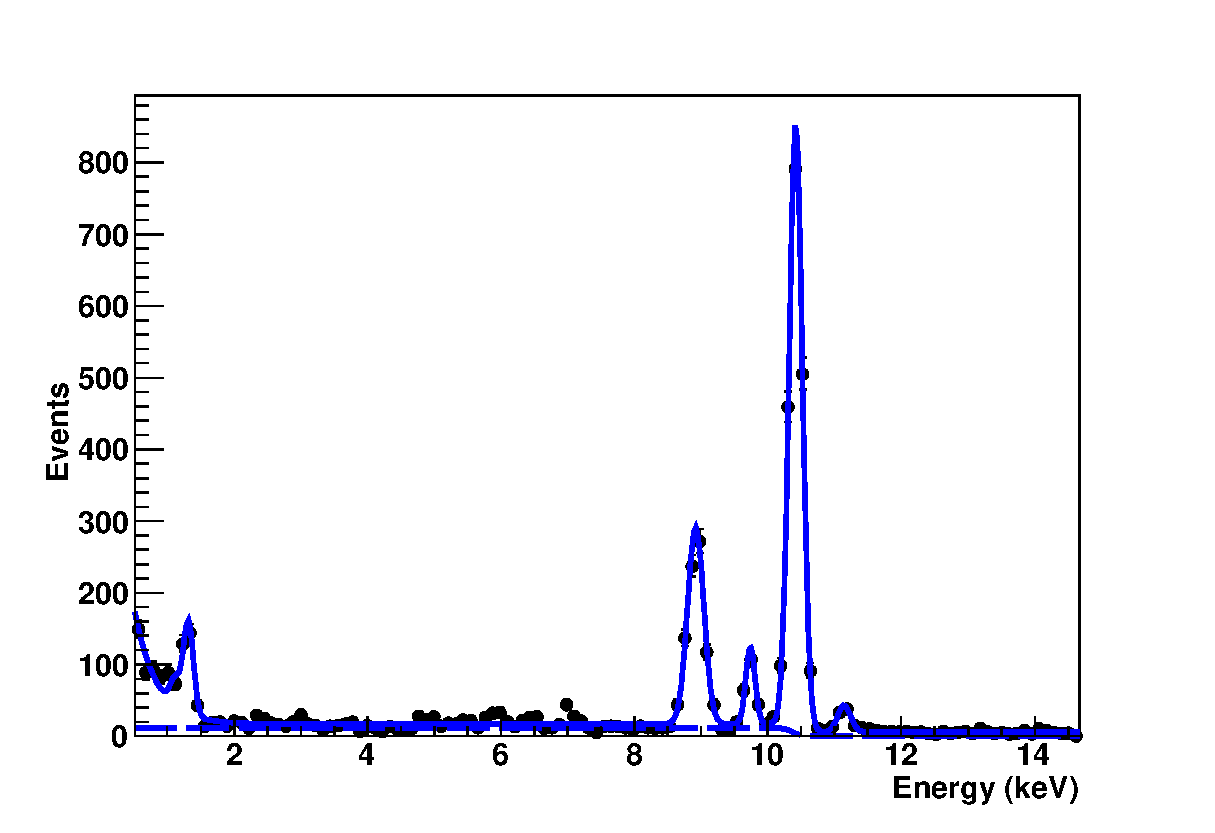
\includegraphics[width=\plotwidth]{HighEnergyFitRun_all_99}					
						}
						\subfigure[High-gain channel] {
							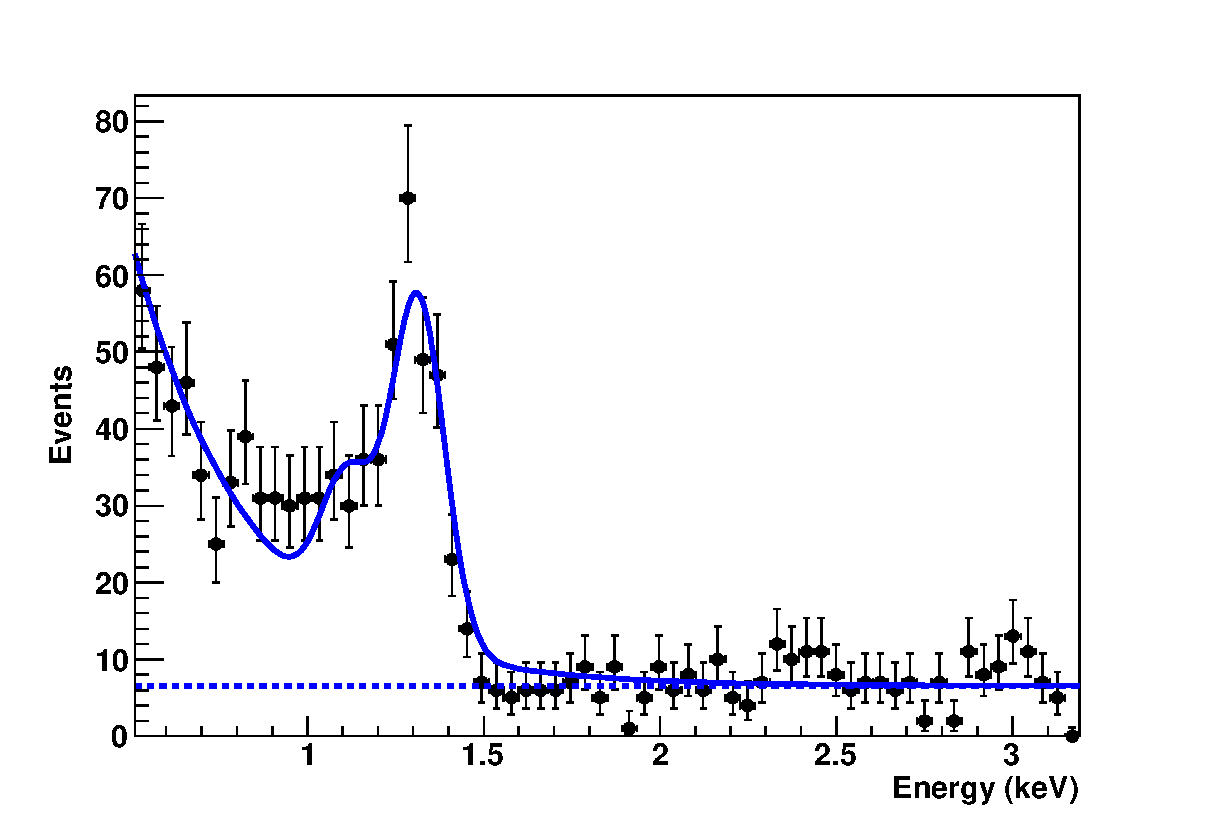
\includegraphics[width=\plotwidth]{LowEnergyFitRun_all_99}
						}
						
						\caption[Example of fits performed to estimate amount cut by rise-time cuts]
						{Example of fits performed to estimate amount cut by rise-time cuts.  These data had the 99\% rise-time cut applied.  The l.ow-gain channel 
						plot includes the error function component of the fit, seen as a dashed line below the x-ray lines.}
						\label{fig:BeGeFitExample}
					\end{figure}


					\paragraph{Low-gain channel results}

The results for the low-gain channel are given in Figure~\ref{fig:RTSimLowGainResults} and in Table~\ref{tab:RTLowGainResults}.  The higher-energy x-rays ($>8$~keV) behave well at the higher acceptance percentages ($\ge$90\%), though the agreement becomes worse at lower acceptances as the lines tend to retain a larger percentage of counts than expected.  This is evident in the figure as the points begin to increase for rise-time cuts of lower efficiency.  The lower-energy L-capture line from \gersixeight~behaves similarly to the higher-energy lines, but it is clear the amplitude of \znsixfive~L-capture line fluctuates significantly.  This is due to the lack of resolution at low energy for this channel, and so the high-gain channel is required to test this cut more precisely.  

The amplitudes of the background components behave generally as expected, showing a reduction significantly greater than 99\% for a 99\%-acceptance rise-time cut.  This suggests that slow pulses comprise a significant portion of the background in the exponential and two flat components.  The slopes of these lines can give us an idea of the relative composition of slow pulse and fast pulse in each component.  For example, if slow pulses are completely removed using the 99\% acceptance cut, then one expects that the quantity \releff~should remain roughly the same for cuts of lower acceptance. This is true for the flat components (`Flat' and `Erfc') for larger acceptance percentages ($\ge90$\%) but the value starts increasing similarly to the results from the high-energy x-ray lines.  This is expected, since the results from the x-ray lines indicate that the cuts retain a larger percentage of events than expected.  However, the two flat components do not behave consistently at lower rise-time cut acceptances, though this is due to a strong correlation between the error function and flat backgrounds.  For example, for low-acceptance very few events remain in the data set and the error function and flat function become indistinguishable.  Despite this, the fact that the \releff~is statistically equivalent for the two background components at higher rise-time acceptances suggests that the cut behaves correctly there.  

The exponential background component exhibits the opposite behavior from the flat background components, decreasing as the rise-time acceptance percentage reduces.  This suggests that slow pulses still remain in this region after rise-time cuts are applied.  However, as noted before, the resolution of this channel is insufficient to test this properly and so this must be verified with the high-gain channel.  Finally, the fit exponential constant, $c_{1}$, demonstrates a marked shift when the rise-time cut is initially implemented, but is consistent between the different rise-time cuts (see Figure~\ref{fig:RTLowGainExpConstant}).  The major shift arises as the 99\% rise-time cut removes many events near threshold and the fact that the value of $c_{1}$ remains consistent as further rise-time cuts are applied suggests that the calculated acceptance contours are consistent near threshold.  

It is possible that the same mechanism which generates the partial charge collection in the `plateau' discussed in Section~\ref{sec:BeGeSpecFit} is related to or the same as that which gives rise to slow-rise-time pulses.  If this were true, we would expect the rise-time cut to significantly reduce or completely remove the contributions to the background from the error function.  The rise-time cut leaves a remaining contribution in the plateau, but this could also be due to deviations between the fit PDF and the data.  One can clearly see this in Figure~\ref{fig:RTLowGainCompResults} comparing two fits to data with a rise-time cut of 95\% and another set with only microphonics cuts.  The significant deviation from the best-fit line of data in the `plateau' region of the spectrum indicates the presence of unaccounted-for backgrounds, in particular possibly other electron-capture cosmogenic species\footnote{Contributions from the continuum of higher-energy processes should already be taken into account by the flat (non-error function) background.}.  The presence of this background does pull the contribution from the error function up.  


						\begin{sidewaysfigure}
							\centering
							\subfigure[X-rays]{
								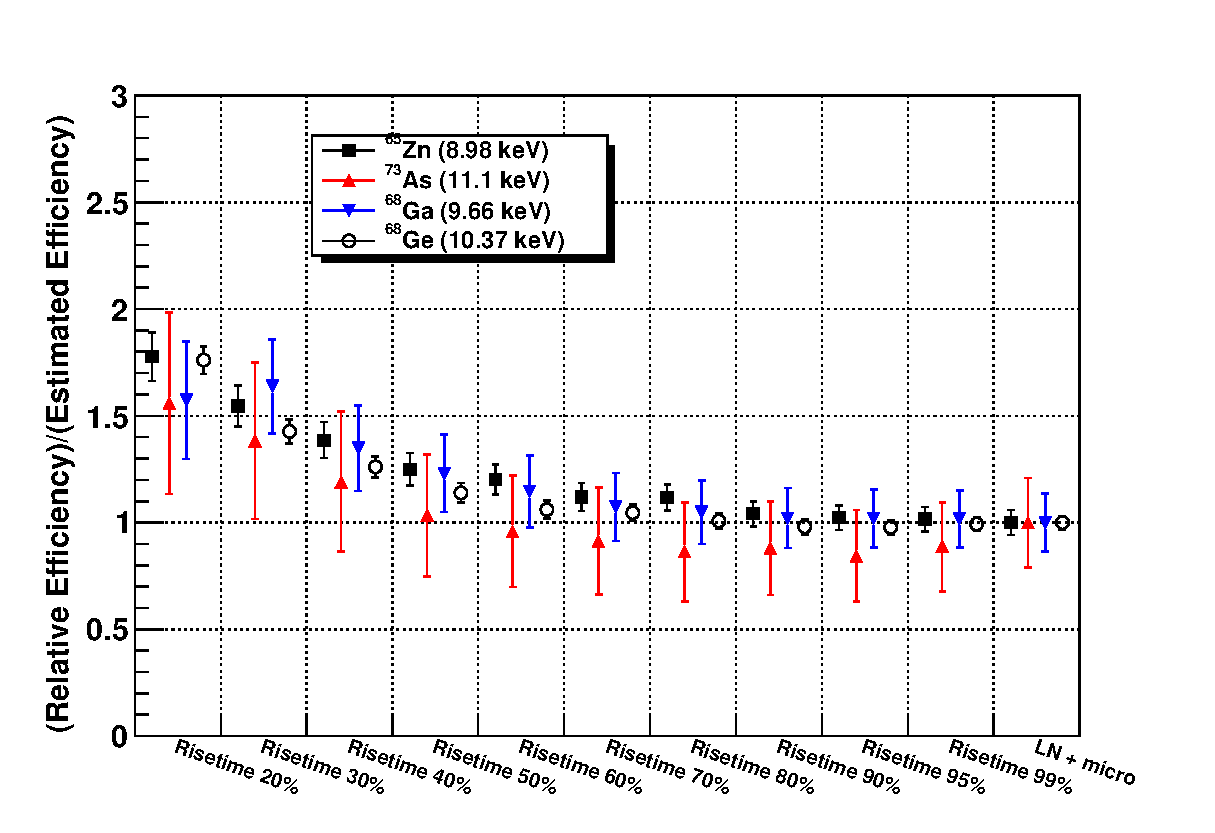
\includegraphics[width=0.46\textheight]{GammaLines}
								\label{fig:RTLowGainXrays}						
							}
							\subfigure[Low x-rays]{
								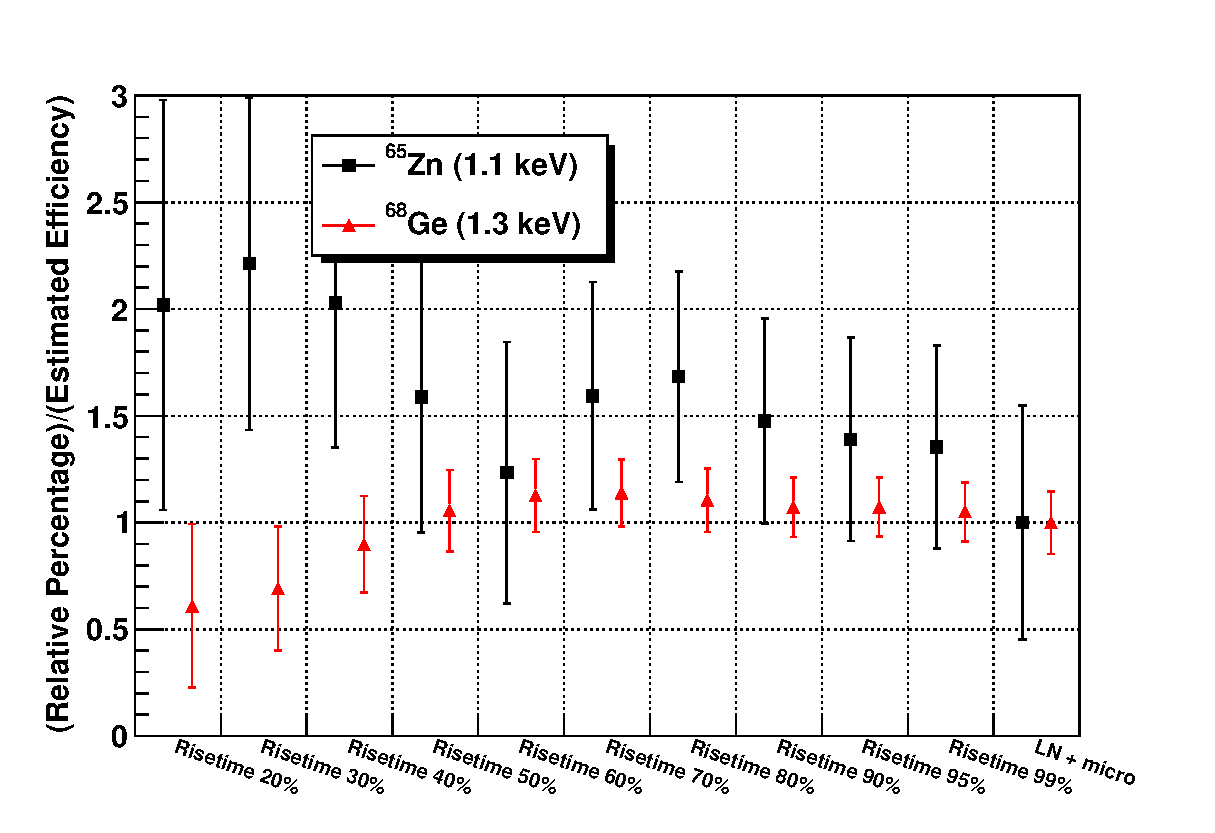
\includegraphics[width=0.46\textheight]{LowHighGammaLines}
								\label{fig:RTLowGainLowXrays}						
							}												
							\subfigure[Background components]{
								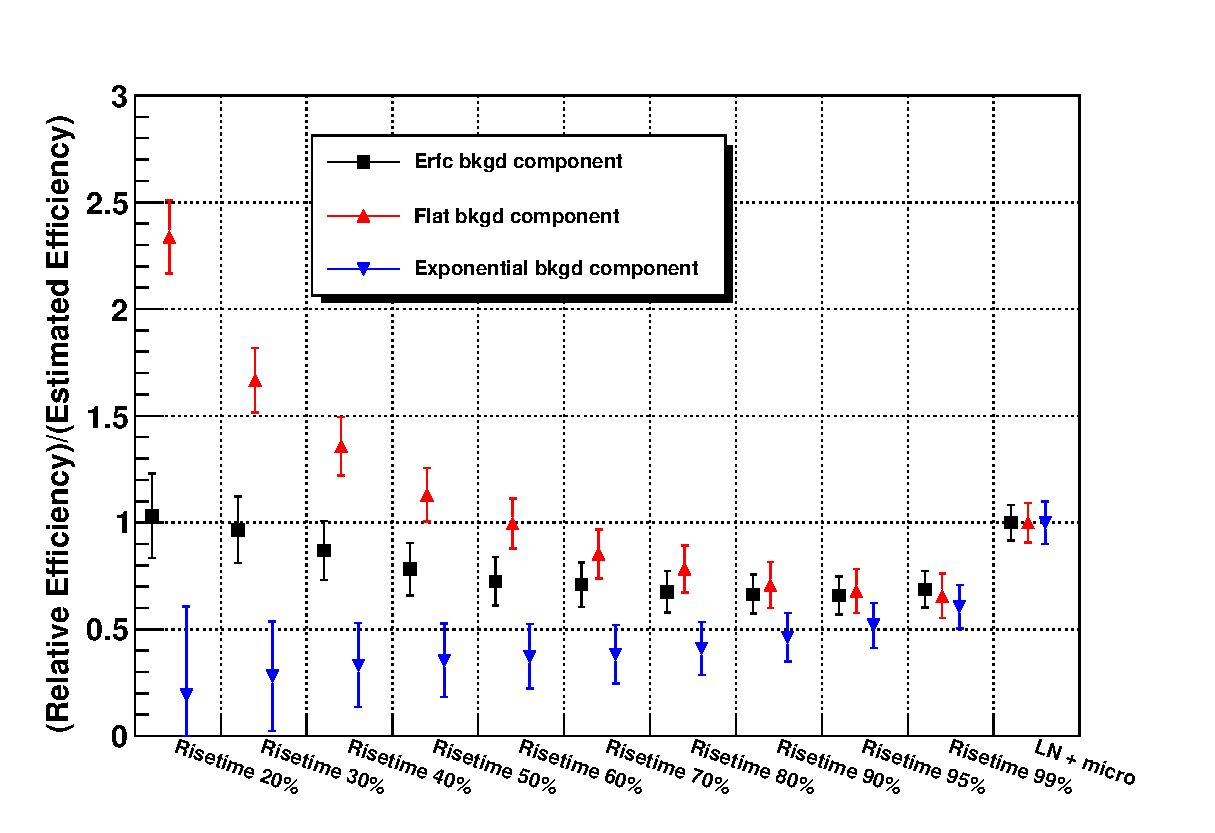
\includegraphics[width=0.46\textheight]{BackgroundComponents}
								\label{fig:RTLowGainBkgd}						
							}
							\subfigure[Exponential Constant, $c_{1}$l]{
								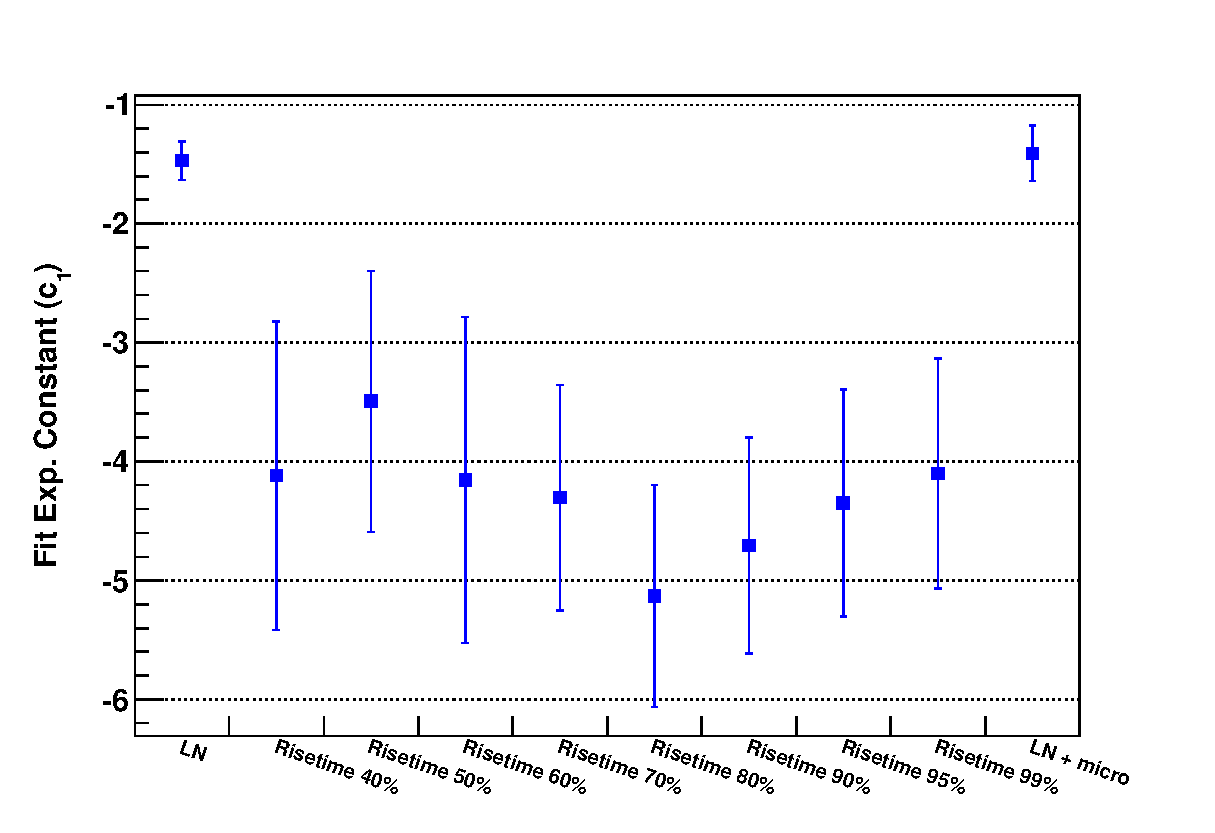
\includegraphics[width=0.46\textheight]{ExpConstant}
								\label{fig:RTLowGainExpConstant}
							}																					
							\caption[Behavior of fit components after cuts for low-gain channel]
							{Behavior of fit components after cuts for low-gain channel.  `LN+micro' refers to data with only
							LN and microphonics cuts applied.  The percentages
							refer to data with a rise-time cut applied with the designated efficiency.}
							\label{fig:RTSimLowGainResults}
						\end{sidewaysfigure}

						\begin{sidewaysfigure}
							\centering
							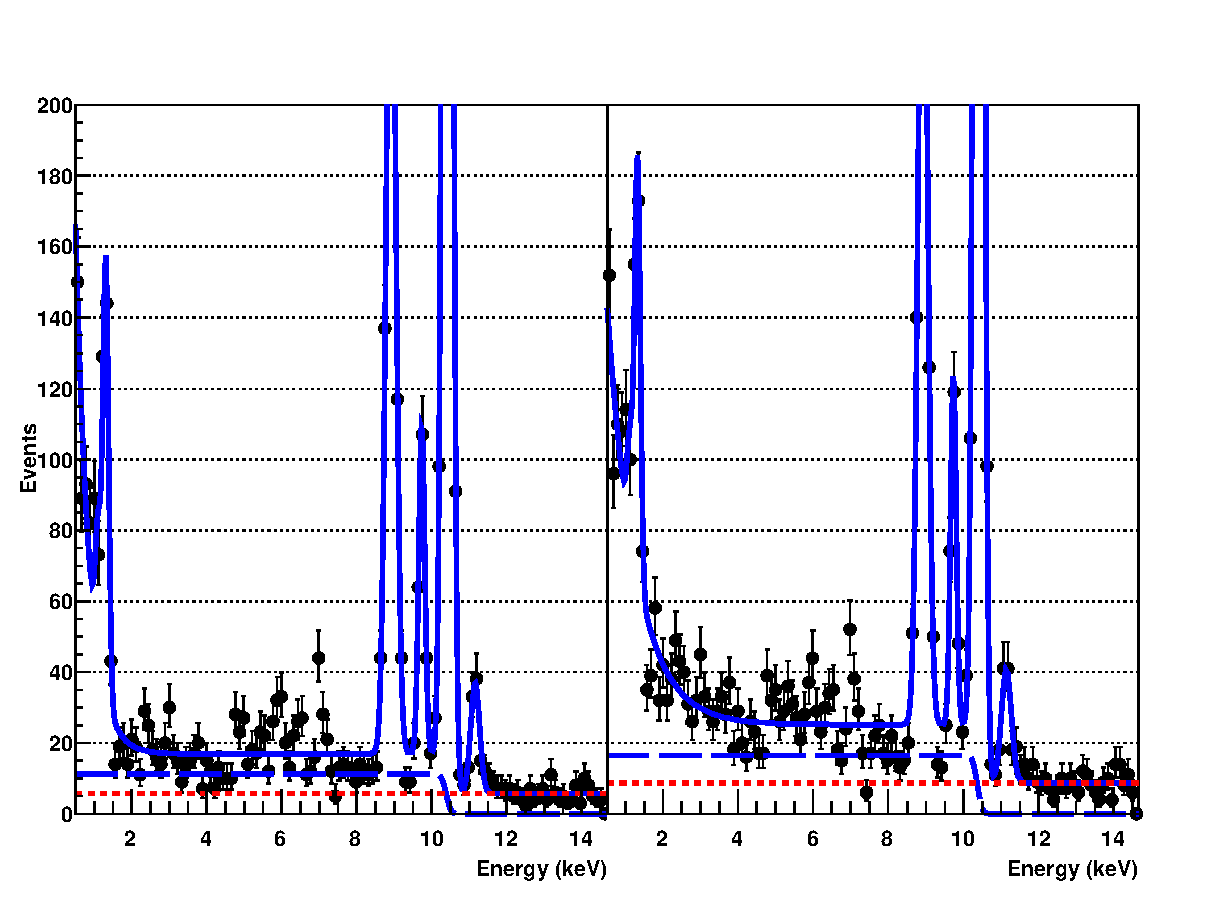
\includegraphics[width=0.9\textheight]{BeGeFitExample}									
							\caption[Comparison of fit to data with 99\% rise-time cut applied and data with only microphonics cuts applied]
							{Comparison of fit to data with 99\% rise-time cut applied (left) and data with only microphonics cuts applied (right).  
							Components from the flat background (red, dotted) and the error function background 
							(blue, dashed) to the overall fit (blue, solid) are shown.  To note is the 
							reduction in flat regions including the `plateau' below the Ge K-capture line.  However, several significant deviations of data from fit remain,
							suggesting the presence of additional background possible from other electron capture species.  See text for details.}
							\label{fig:RTLowGainCompResults}
						\end{sidewaysfigure}
						
						\begin{sidewaystable}
							\centering
							\footnotesize
							\begin{tabular}{l  r@{$~\pm~$}l  r@{$~\pm~$}l  r@{$~\pm~$}l  r@{$~\pm~$}l  r@{$~\pm~$}l  r@{$~\pm~$}l  r@{$~\pm~$}l  }
								\toprule 
								& \multicolumn{14}{c}{Components (counts)} \\
								\cmidrule[1pt]{2-14} 
								Cut & \multicolumn{2}{c}{$^{65}$Zn (8.98 keV)} & \multicolumn{2}{c}{$^{68}$Ga (9.66 keV)} & \multicolumn{2}{c}{$^{68}$Ge (10.37 keV)} & \multicolumn{2}{c}{$^{73}$As (11.1 keV)} & \multicolumn{2}{c}{Erf bkgd} & \multicolumn{2}{c}{Exp bkgd} & \multicolumn{2}{c}{Flat bkgd}  \\
								\midrule
							        	 Risetime 20\% & 264.9 & 17.9 & 52.8 & 8.9 & 681.3 & 26.8 & 29.9 & 7.9 & 302.9 & 44.7 & 31.8 & 12.1 & 520.1 & 47.8  \\
									 Risetime 30\% & 345.9 & 20.3 & 82.4 & 10.9 & 828.9 & 29.5 & 39.8 & 9.8 & 425.5 & 48.8 & 69.1 & 15.3 & 555.8 & 51.7  \\
									 Risetime 40\% & 413.2 & 22.1 & 90.4 & 11.5 & 976.0 & 32.0 & 45.7 & 10.5 & 510.3 & 51.9 & 109.1 & 17.7 & 604.1 & 54.6  \\
									 Risetime 50\% & 465.6 & 23.4 & 103.2 & 12.2 & 1102.8 & 34.0 & 49.6 & 9.5 & 573.9 & 52.1 & 145.3 & 20.5 & 628.9 & 52.7  \\
									 Risetime 60\% & 537.4 & 25.0 & 115.2 & 13.0 & 1232.4 & 35.9 & 55.1 & 9.8 & 638.9 & 53.8 & 183.9 & 22.3 & 665.0 & 53.8  \\
									 Risetime 70\% & 583.8 & 26.1 & 125.9 & 13.5 & 1417.7 & 38.4 & 61.3 & 10.7 & 728.9 & 55.6 & 219.5 & 23.8 & 664.9 & 55.3  \\
									 Risetime 80\% & 666.0 & 27.7 & 140.7 & 14.2 & 1559.8 & 40.3 & 66.2 & 10.8 & 793.1 & 57.2 & 268.5 & 25.6 & 697.3 & 56.3  \\
									 Risetime 90\% & 698.2 & 28.4 & 153.9 & 14.8 & 1706.7 & 42.1 & 76.0 & 11.7 & 877.5 & 59.2 & 340.1 & 29.1 & 707.8 & 57.7  \\
									 Risetime 95\% & 724.7 & 28.9 & 162.5 & 15.1 & 1796.9 & 43.2 & 77.0 & 11.6 & 919.0 & 59.6 & 403.3 & 31.2 & 718.2 & 57.3  \\
									 Risetime 99\% & 749.8 & 29.5 & 168.7 & 15.5 & 1903.4 & 44.4 & 84.2 & 12.2 & 999.9 & 61.9 & 491.2 & 35.5 & 724.2 & 58.6  \\
									 LN + micro & 745.1 & 30.4 & 167.6 & 16.3 & 1935.5 & 45.2 & 95.9 & 14.2 & 1467.7 & 85.7 & 818.1 & 57.2 & 1112.4 & 72.9  \\
								 
								\bottomrule
							\end{tabular}

							\caption[Behavior of fit components after cuts for low-gain \bege~channel]
							{Behavior of fit components after cuts for low-gain channel.  Components are given in total counts.}
							\label{tab:RTLowGainResults}
						\end{sidewaystable}						

					\paragraph{Low-energy results}

Results for the high-gain channel are shown in
Figure~\ref{fig:RTSimHighGainResults}. The conclusions for this channel set are
similar to the low-gain channel set.  The enhanced resolution of the
high-gain channel has reduced the size of the error bars for the L-capture
lines and \releff~behaves very similarly to the low-gain channel for higher
rise-time acceptances.  Additionally, the behavior of the exponential constant
is consistent in this channel as with the low-gain channel except with the 20\%
rise-time cut data.  In this particular instance, the fit actually fails and
runs up against the parameter limit for the exponential constant.  This failure
occurred due to insufficient counts remaining in the data set resulting in the
two background components looking too much alike.

In this channel, only two background components, flat and exponential, remained since the energy range did not exceed 3.5~keV.  \releff~with 20\% rise-time cut data is distorted because the two background components look alike, rendering results from this data set incomparable to the other sets.  The \releff~of the flat component behaves well at higher rise-time acceptances, remaining flat for acceptances $\ge80$\%.  However, for the exponential component, \releff~reduces with decreasing rise-time acceptance, possibly indicating the cut does not \emph{fully} remove background from slow-rise-time pulses.  If one considers the measured rise-time distribution for the high-gain channel in Figure~\ref{fig:RisetimeDataVsCutHighGain} with an included 99\% cut line, it is clear that the cut begins to break down near threshold.  
This is not unexpected, since as the signal-to-noise of the pulse reduces de-noising will have less and less of an effect and the ability to measure the rise-time of pulses effectively will diminish.

						\begin{sidewaysfigure}
							\centering
							\subfigure[Exponential Constant, $c_{1}$l]{
								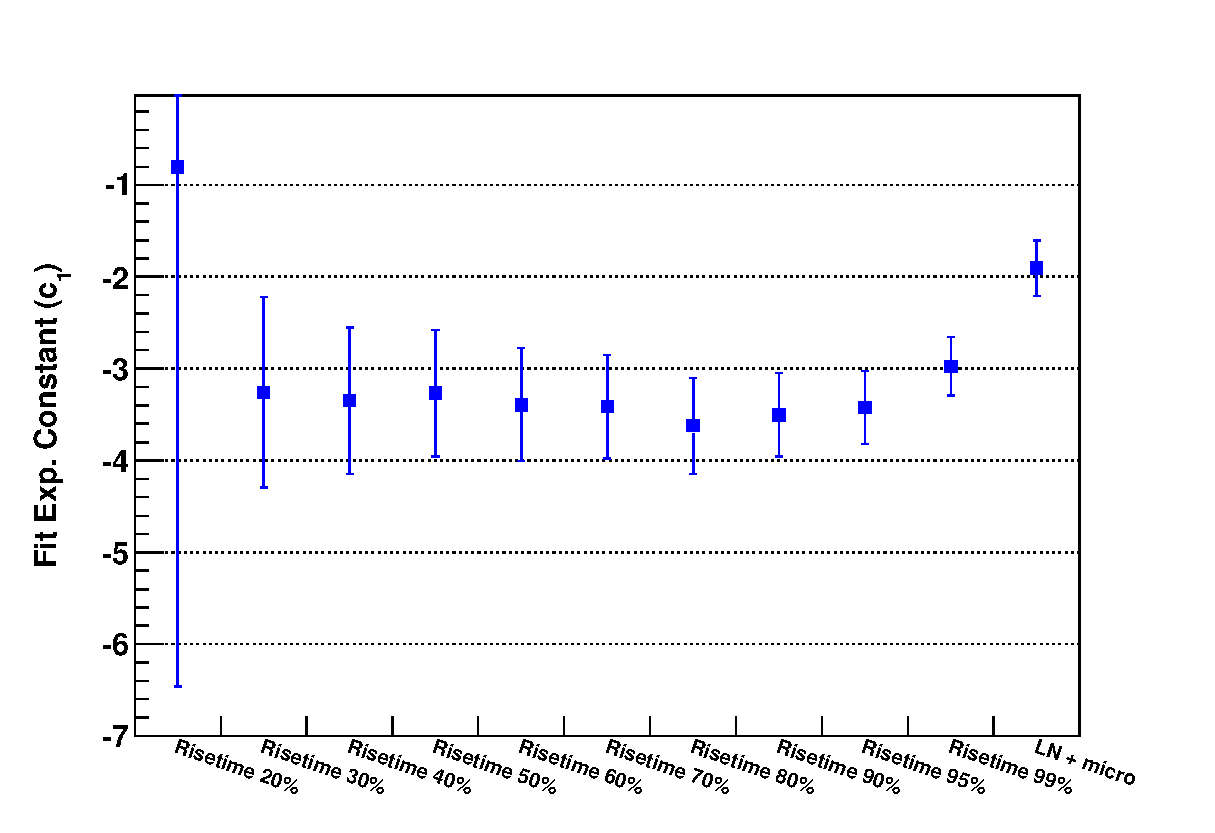
\includegraphics[width=0.46\textheight]{LowExpConstant}
								\label{fig:RTHighGainExpConstant}
							}
							\subfigure[X-rays]{
								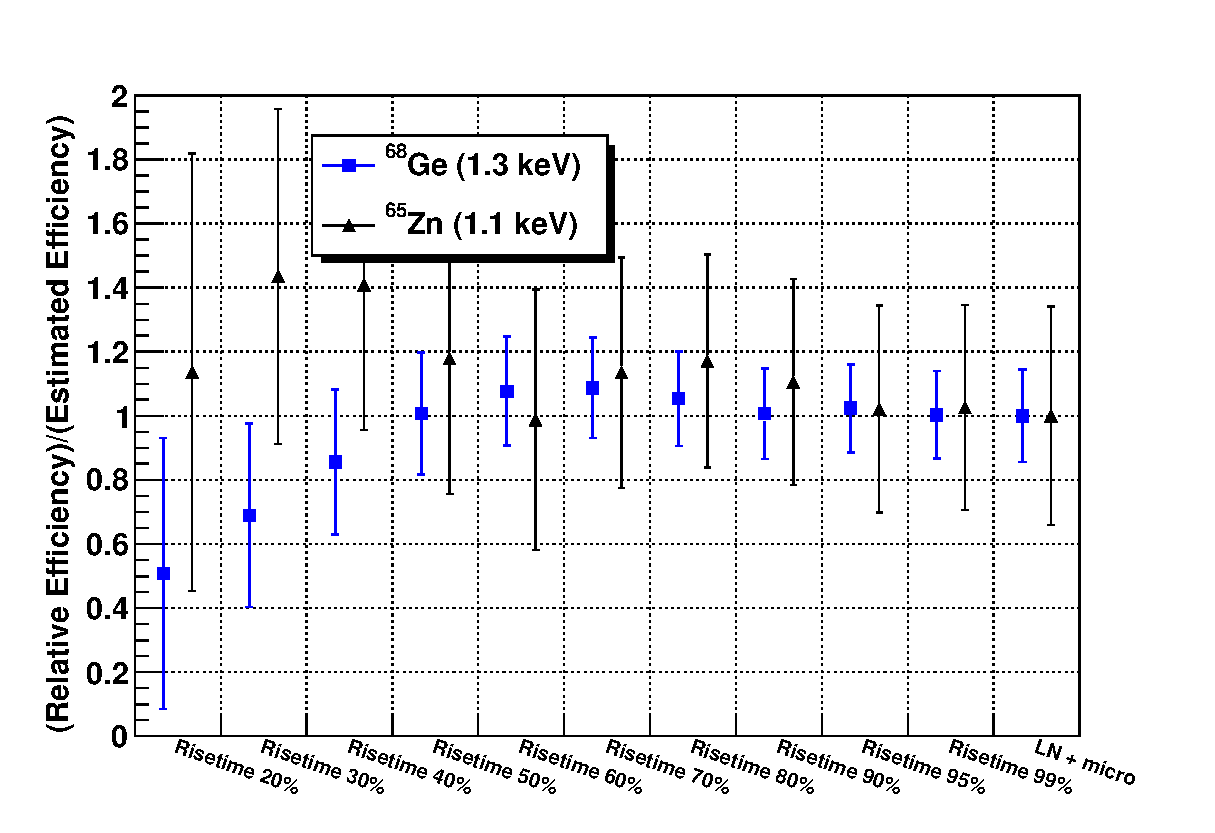
\includegraphics[width=0.46\textheight]{LowGammaLines}
								\label{fig:RTHighGainXrays}						
							}		
							\subfigure[Background components]{
								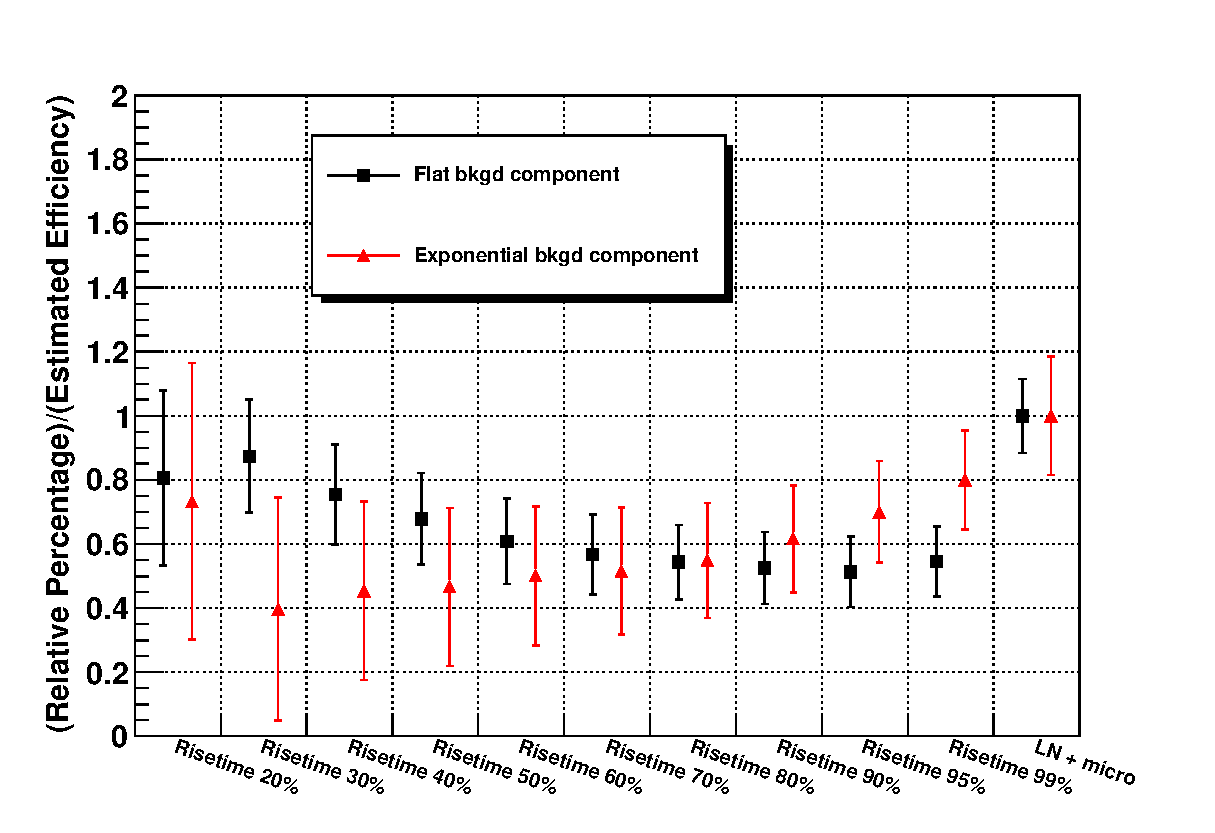
\includegraphics[width=0.46\textheight]{LowBackgroundComponents}
								\label{fig:RTHighGainBkgd}						
							}														
							\caption[Behavior of fit components after cuts for high-gain \bege~channel]
							{Behavior of fit components after cuts for high-gain channel.  `LN+micro' refers to data with only
							LN and microphonics cuts applied.  The percentages refer to data with an rise-time cut applied
							with the designated efficiency.}
							\label{fig:RTSimHighGainResults}
						\end{sidewaysfigure}
						
						\begin{sidewaystable}
							\centering
							\begin{tabular}{l  r@{$~\pm~$}l  r@{$~\pm~$}l  r@{$~\pm~$}l  r@{$~\pm~$}l  }
								\toprule 
								& \multicolumn{8}{c}{Components (counts)} \\
								\cmidrule[1pt]{2-8} 
								Cut & \multicolumn{2}{c}{$^{65}$Zn (1.1 keV)} & \multicolumn{2}{c}{$^{68}$Ge (1.3 keV)} & \multicolumn{2}{c}{Exp bkgd} & \multicolumn{2}{c}{Flat bkgd}  \\
								\midrule
							        	 Risetime 20\% & 18.3 & 7.7 & 21.0 & 7.4 & 83.2 & 26.4 & 125.5 & 25.3  \\
									 Risetime 30\% & 34.7 & 9.8 & 42.8 & 9.3 & 67.7 & 17.1 & 203.8 & 19.1  \\
									 Risetime 40\% & 45.4 & 11.0 & 70.7 & 11.1 & 103.3 & 19.1 & 234.5 & 20.5  \\
									 Risetime 50\% & 47.5 & 11.9 & 104.1 & 12.9 & 132.5 & 21.5 & 263.9 & 21.9  \\
									 Risetime 60\% & 47.7 & 12.5 & 133.6 & 14.3 & 170.8 & 23.2 & 283.8 & 22.7  \\
									 Risetime 70\% & 64.0 & 13.8 & 157.2 & 15.4 & 205.1 & 25.0 & 308.7 & 23.8  \\
									 Risetime 80\% & 75.5 & 14.7 & 174.3 & 16.2 & 249.7 & 26.2 & 337.5 & 24.5  \\
									 Risetime 90\% & 80.2 & 15.8 & 187.1 & 17.1 & 315.0 & 29.5 & 367.7 & 26.1  \\
									 Risetime 95\% & 78.2 & 16.2 & 201.1 & 17.7 & 377.7 & 31.7 & 379.0 & 26.7  \\
									 Risetime 99\% & 81.9 & 17.2 & 205.4 & 18.4 & 450.5 & 36.5 & 419.3 & 29.6  \\
									 LN + micro & 80.6 & 19.4 & 206.7 & 21.2 & 568.4 & 74.5 & 777.7 & 63.7  \\
								 
								\bottomrule
							\end{tabular}


							\caption[Behavior of fit components after cuts for high-gain \bege~channel]
							{Behavior of fit components after cuts for high-gain channel.  Components are given in total counts.}
							\label{tab:RTHighGainResults}
						\end{sidewaystable}

		\subsubsection{Conclusions and discussion}
		\label{sec:RTBeGeConclusions}
		
Evidence from past results~\cite{Strauss196780,Sakai:1971ff} and recent results presented in~\cite{Aalseth:2010aa} suggest that slow pulses can arise due to poor charge collection from weak electric fields in the dead layer of the n$^{+}$ Li contact.  These results also suggest that energy information of the initiating event is lost so that these slow pulses can comprise a background at low energy, though one of not-yet-precisely-determined distribution.  The conclusions from these references were determined by scanning a source of low-energy gammas (\amtwofourone, 59.5~keV gamma) around the outside n$^{+}$ contact of the detector (the detector geometries varied in the references) and determining the distribution of rise-times for recorded events.  The low energy of the americium source ensured that a majority of the gammas deposited energy in or near the outer contact.  The resulting rise-time measurements demonstrated a substantial distribution of slow rise-time pulses, supporting the conclusion that at least a component of these slow-rise-time events come from energy deposition at or near the outer contact.  

Another measurement performed using the different, but similar \ppc~detector~\cite{Barbeau:2009fk} measured the rate versus time at low energies in several energy regions, watching the decay of \gersevenone~(11.4~day half-life).  This measurement focused on three main regions: the Ge K-capture line (10.367~keV), the Ge L-capture line (1.3~keV), and the flat region in between ($2\to6$~keV).  The results found that the decay of counts in the flat region matched the decays of counts in the L- and K-capture regions, suggesting partial energy deposition from the \gersevenone~decay below 10.367~keV.  It is possible that this result is related to the slow-rise-time pulses, in particular that decays of \gersevenone~near the outer contact resulted in both slow pulses and partial charge collection, but no such data were taken during this measurement.  To firmly establish the equivalency of these results, it is essential to measure the rise-time of the preamplifier traces, remove slow pulses, and produce the resulting counts vs.~time for the region between the L- and K-capture lines.  If partial energy deposition is arising in the same process producing the slow pulses, the removal of slow-pulse events should result in the flattening of the counts vs.~time curve for the energy region between the capture lines.  Unfortunately, for this analysis preamplifier traces were only recorded following the decay of the majority of \gersevenone~and the slow decay of \gersixeight~(271~days) yields insufficient statistics over a short period of time to measure this well.  The relative content of \gersevenone~in the detector could be increased through activation by either bringing the detector to the surface or introducing a neutron source, but such a test cannot be performed until the conclusion of the counting runs.  

Whereas it is likely that a component of these slow pulses is arising from charge deposition near the crystal outer contact, it is important to determine other possible sources of these events.  For example, surface channel effects, i.e.~distortion of crystal fields through charge collection on the passivated surface, might produce similar results.  One could use the extreme sensitivity of the surface channel to temperature detailed in~\cite{Hull1995488} to determine if the population of slow-rise-time events changes with temperature.  Additionally, characterization measurements using a low-energy gamma source must be performed for several other \ppc~detectors to determine how sensitive the distribution of slow-rise-time events is to manufacturing and geometry differences.  

Whatever the origin of these slow-pulse events, it is clear that they can produce a background to low-energy signals.  If the majority of these slow pulses arise from energy deposition near the outer surface, a cut on rise-time would effectively generate a cut on the fiducial volume and mass of the detector.  Understanding the active fiducial volume of the detector is critical for experiments sensitive to mass exposure times, such as those searching for $\nonubb$ or dark matter.  For double-beta decay, even though $\qval$ is around 2~MeV, the decay is internal to the detector and energy is deposited by two electrons summing to $\qval$.  The range of electrons at this energy is on the order of 1~mm, so it is expected that poor charge collection in an outer layer of the detector could still have an effect on a fiducial mass for $\nonubb$ results.  


	\subsection{Extracting or looking for signals in cut data}
	\label{sec:BeGeLowEnergyFeatures}
	
	The ultimate goal of introducing a cut to a data set is to remove events to enhance the signal-to-noise ratio of the data set.  In this particular analysis, work focused on removing `noise' events that might populate the energy region near threshold because this energy region is critical for deriving exclusion limits for dark matter.  With many analyses, it is common to study cuts by choosing in parameter space a background region or set of regions and a background+signal region, preferably bookending the background+signal area with background-only regions to avoid any sort of boundary effects.   This analysis explored rise-time cuts in a similar manner: calculate what you should see when you take a cut and see if the result matches your expectations.  For higher-rise-time-cut acceptances, the calculation proved a sufficient model.  
	
	
	Understanding the data at low energies proves difficult for several reasons: (1) we do not know the exact energy distribution of slow pulses; (2) the most critical region, energies near threshold, is inherently a boundary region; and (3) a complete interpretation of slow pulses and their origin in this particular detector is missing.  Addressing these points is important to using this data for physical interpretation:
	
	\begin{enumerate}
		\item Whereas the exact energy distribution of slow pulses for this detector is unknown, we can infer something about the population through the systematic results.  In particular, the flat background components of the data essentially parameterizing the range $1.5\to14.5$~keV, behaved as one would expect if \emph{all} slow pulses were cut using the 99\% rise-time cut.  In contrast the exponential component, parameterizing the population from threshold to $\sim$1.5~keV, behaved as if the 99\% rise-time cut did not remove all slow-pulse events.  
		\item Near threshold, the two x-ray lines at 1.1 and 1.3~keV provide a test of the validity of the model, and these lines behaved well with the cuts.  Additionally, the insensitivity of the exponential constant to different rise-time cuts implies that the calculated cut lines at different acceptance percentages were consistent until the threshold.  However, it does \emph{not} necessarily imply that slow-rise pulses were fully removed.  The same result can be expected if slow and fast pulses occupy a similar rise-time distribution in this energy region due to limitations of the rise-time calculation at low signal-to-noise ratios.
		\item Evidence suggests that at least a portion of these slow pulses arise from energy deposition near the outer contact
		and therefore a rise-time cut would require a reduction in fiducial mass.  Even if not all slow pulses are generated by this
		mechanism, the assumption that they are is considered conservative .  
	\end{enumerate}
	
	Points 1 and 2 relate to one another and both suggest that the region near threshold could still be contaminated with slow-rise-time pulses.  The presence of additional uncut events here could explain the general exponential shape seen in the data especially considering that the calculated acceptance line necessarily increases as it nears threshold (see Figure~\ref{fig:RisetimeDataVsCut}).  Other explanations of this feature could be considered as well: (1) a population of events arising from a modulation of noise; (2) uncut microphonics; and (3) presence of an exponential signal from, for example, a WIMP source or some other unknown background.  The first two possibilities should exhibit characteristic time signatures in events near threshold; in particular, they should arrive with a rate that varies with time over short time scales.  The presence of time variation in the data is explored in the following section (Section~\ref{sec:BeGeTimeCorrelations}).  It is also possible to measure the noise profile over time by generating random triggers, but this was not performed for this detector.  The third explanation coupled with the understanding that slow-rise-time pulses could still populate near threshold suggests that any analysis of this near-threshold region must treat it with care, conservatively foregoing any claims other than exclusion limits.  The extraction of a limit on a signal in the presence of unknown background is explored in the following chapter, in particular Section~\ref{sec:LimitsUnknownBackgroundML}.  
	
	Following point 3, for this analysis and for the purpose of estimating the mass of the detector we assume that either all or a significant majority of slow-rise-time events are coming from energy deposition near the surface.  We therefore assume that the detector includes an outer dead layer within the outer Li contact, followed by a transition layer with weak electric fields.  We can calculate the width of this transition region through two methods and compare, in particular using the results of the rise-time systematic tests described earlier as well as another calculation presented in~\cite{Aalseth:2010aa}.  If we assume a majority of the slow-rise events in the `plateau' beneath the Ge K-capture line come from partial charge collection of the energy deposited from these electron-capture decays, then the percentage of volume of the detector in which these slow-pulse events occur may be estimated as follows:  calculate the sum of events in the prominent x-ray lines at high energy, $ y = \sum_{i} N_{i}$ where $i$ includes \gersixeight, \galsixeight, \znsixfive, and \asseventhree, and then calculate the difference in counts, $\Delta x$, between events in the error function distribution before and after a 99\% rise-time cut, properly adjusting for the expected efficiency of the cut (99\%).  The value, $\frac{\Delta x}{\Delta x + y}$ is then the fraction of volume affected by slow-pulse generation with respect to the total active volume of the detector.  The values $\Delta x$ and $y$ were measured as $457.7\pm105.9$ and $3401.8\pm121.3$, respectively, yielding an affected fraction of active volume of $0.135\pm0.031$.  The active volume can be estimated by assuming an outer dead layer of 1~mm, reducing the 0.44~kg total mass to an active mass of 0.4~kg.  Therefore, the final fiducial mass after rise-time cuts would be assumed to be $0.346\pm0.0124$~kg.  This estimation ignores any effect from the passivated surface of the detector.

	We may compare this to a separate estimation presented in~\cite{Aalseth:2010aa}.  This particular measurement coupled a source scan with \amtwofourone~with a simulation to estimate the dead layer plus transition region in a different but similar \ppc~detector.  The results of this measurement suggested an outer dead layer of 1~mm, plus a transition layer of 1~mm yielding a total active volume of 0.33~kg.  This measurement agrees with the above estimation and to remain conservative the smaller value will be used in the later presented analyses.
	
	When fitting to cut data, it is important to take into account the efficiencies of each cut.  The total energy-dependent efficiency can be defined by the equation:
		\begin{equation}
		f_{eff}(E) = f_{Trigger}(E) \prod_{i~\in~\left\{cuts\right\}} f_{i}(E)		
		\label{eqn:EfficiencyEquation}
		\end{equation}
where $f_{Trigger}(E)$ is the trigger efficiency defined in Equation~\ref{eqn:TrigEfficiency}, and the product is over all cuts taken.  The efficiency of the microphonics cut was estimated as $f_{micro} = 0.997$ and the rise-time efficiencies are estimated as equivalent to the acceptance percentage.  This assumption is valid for higher rise-time acceptances, $\ge80$\%, and conservative for lower percentages.  The efficiency function is used to determine the weight of an event at a particular energy, given by $w(E) = 1/f_{eff}(E)$.

	\section{Time correlations and systematics}
	\label{sec:BeGeTimeCorrelations}

	Searching for time dependence of parameters and any possible time correlation of events provides a powerful systematic test of the data.  Small deviations in detector health (e.g.~noise, baseline shifting, etc.) can have a more marked effect on events near threshold.  For example, a change in noise or a shift in baseline could affect the triggering efficiency, modifying the collection probability for events near threshold.  Additionally, searching for time correlations provides a metric for ensuring that data collection is behaving appropriately and as expected.  In addition to tracking detector health parameters, it is important to analyze event rates and times between events to look for any deviation from Poisson statistics.  Such deviations could arise from environmental changes or events.  For example, nearby work in the experimental hall generating additional vibration could increase microphonics events, or an introduction of a hot source in the shared lab space could increase count rates.  Finally, it is possible to perform tests in combined energy-time space looking to see if classes of events (e.g.~events in a certain energy range) have correlations \emph{outside} their class region.  An obvious example of this is a decay chain, in which an initial energy deposition from a parent is correlated in time with another event at different energies from the decay of the daughter.  Whereas these types of correlations between decay chains should show up in the data, the discovery of other correlations of unknown origin could point to a potential source of event contamination.  
	
		\subsection{Detector health versus time}
		\label{sec:BeGeParsVsTime}

	In contrast to the previous data run with \ppc2, fewer parameters were tracked during the lifetime of the experiment (see Section~\ref{sec:PPC2DetParsVsTime}).  In particular, due to limited channels in the DAQ electronics the trigger efficiency was not monitored with automated tests nor was the rate of the reset electronics recorded.  In general, both these parameters are important to catalogue since they could affect the signal region near threshold.  However, due to the strong correlation of the reset rate on  the measured baseline in unshaped pulses seen in the results of Section~\ref{sec:PPC2DetParsVsTime}, the baseline can be used as a proxy to ensure that the reset rate did not change significantly.  Similarly, it was possible to monitor the noise by using the measured RMS of the baseline to determine whether it changed significantly over time.  
	
	The baselines of two channels were tracked, channel 1 (shaped) and channel 5 (unshaped preamp trace).  For every day of run-time, the calculated baselines were binned and fit to a gaussian.  
%As discussed before in Section~\ref{sec:BeGeBaseline}, 
The binned baseline data included outliers in one direction which were attributed to having come from the return of the baseline to its nominal value following a reset event in the preamplifier.  Since these outliers were a low percentage of the total events, only one gaussian was fit to the binned baseline data.  From these fits, the mean and $\sigma$ values were extracted and the relationship of these parameters versus time are plotted in Figure~\ref{fig:BeGeBaselineData}.  An inspection of the results reveals that the $\sigma$ values from both unshaped and shaped channels were stable with time.  In contrast, the mean value of the baseline in the unshaped channel demonstrates variation, but this is not mirrored exactly in the mean of the baseline calculated from the shaped channel.  This is likely due to baseline restoration electronics in the spectroscopy amplifier which render the baseline of the output less sensitive to baseline modulation of the input.  Regardless, it is evident that the noise of the baseline does not change significantly in either the shaped or unshaped channels over the time range of the experiment.  This suggests that the trigger efficiency and electronic noise remained similarly unchanged throughout the time of the experiment.  

			\begin{sidewaysfigure}
				\centering
				\def\figwidth{0.45\textheight}
				\newcommand{\plotname}[2]{Baseline#1haped#2}			
				\subfigure[Unshaped channel, mean]{
					\includegraphics[width=\figwidth]{\plotname{Un}{Mean}}
					\label{fig:\plotname{Un}{Mean}}
				}				
				\subfigure[Unshaped channel, $\sigma$]{
					\includegraphics[width=\figwidth]{\plotname{Un}{Sigma}}
					\label{fig:\plotname{Un}{Sigma}}
				}
				\subfigure[Shaped channel, mean]{
					\includegraphics[width=\figwidth]{\plotname{S}{Mean0}}
					\label{fig:\plotname{S}{Mean}}
				}				
				\subfigure[Shaped channel, $\sigma$]{
					\includegraphics[width=\figwidth]{\plotname{S}{Sigma0}}
					\label{fig:\plotname{S}{Sigma}}
				}		
				\caption[Baseline mean and $\sigma$ versus time]
				{Baseline mean and $\sigma$ versus run time for both shaped and unshaped preamp traces.}
				\label{fig:BeGeBaselineData}
			\end{sidewaysfigure}
	
		\subsection{Rates in energy regions}
		\label{sec:BeGeRate}	
		
		Several tests can be performed to analyze the Poisson nature of the data: (1) event rate in an energy region; (2) time difference between events in an energy region; and (3) forward and backward time difference between events occurring in an energy region and \emph{any} other events.  All of these tests should be made with different cuts applied (see Section~\ref{sec:BeGeCuts} for a description of the cuts) since an analysis cut may preferentially remove a portion or an entire population of correlated events.  Therefore, for these tests several cuts were used including the minimal cut (LN fill cut), microphonics cuts and rise-time cuts of varying acceptances.  To perform all these tests, events were selected in particular energy regions: $0.45\to0.55$ keV, $0.5\to1$ keV, $1\to2$ keV, $3\to8$ keV, and $10\to10.76$ keV.  The first two regions tested around and just above threshold, the next two tested regions not significantly populated with $\epsilon$ decays, and the final examined a region symmetric around the mean of the Ge K-capture x-ray (10.367~keV).
		
	During LN fills, all events are vetoed and this could, in principle, generate a significant distortion to any calculated Poisson rates.  However, since the amount of time vetoed during an LN fill is small compared to the measurement time this has little effect on the results.  This can be seen by considering that the probability that one or more events will happen in a certain time period, $\tau$, is $1 - \exp(-\lambda_{\tau})$, where $\lambda_{\tau}$ is the average count rate over that time period.  If we consider that the time vetoed during an LN fill is $\sim15$~minutes, and these fills happen once every two days, the expected number of times one or more events occurs during the roughly 160 day run period is $\sim80 (1 - \exp(-\lambda_{\tau}) )$.  Additionally, the percentage of events affected (events affected/events expected) is given by $\frac{1}{192 \lambda}\left(1 - \exp(-\lambda)\right)$.  The maximum total rate for any of these regions is less than 1 count per 15 minutes, meaning that the percentage of events affected is less than 0.5\%.  Since all other cuts (microphonics and rise-time cuts) should have no time dependence (assuming that slow rise-time events and microphonics events occur randomly and independently), it is expected that rates calculated from data with these cuts applied should be slower, but still Poisson in nature.  
	
	The first test involves analyzing the event rates in a given energy window.  The data were windowed in 8-hour bins and the numbers of counts in the different energy regions were calculated for each of these 8 hours.  Any 8-hour time periods with less than 100\% live-time (i.e.~8 hour runs during which an LN fill occurred) were removed from the data set.  The number-of-counts-seen was histogrammed and fit with a Poisson distribution to extract the rate.  Examples of these fits are shown in	Figure~\ref{fig:BeGeRateFits} and a summary of the fits, including extracted rate and goodness-of-fit, is given in Table~\ref{tab:BeGeFitRates}.  These results indicate that the regions selected behave as expected, demonstrating count rates that follow Poisson distributions.  Additionally, as expected the count rates were reduced with the introduction of cuts while retaining a Poisson shape.  
	
			\begin{table}
				\centering
				\begin{tabular}{r@{$~\to~$}l r@{$~\pm~$}l  c  c  c} 
					\toprule 				
					\multicolumn{2}{c}{Range (keV)} & \multicolumn{2}{c}{$\lambda$ (cts / hr)} & $\chi^2$ & NDF & P-Value \\
					\midrule
					\multicolumn{7}{l}{\emph{LN}} \\
					0.45 & 0.55 & 0.046 & 0.004 & 6.08296 & 2 & 0.0477643 \\
					0.5 & 1 & 0.158 & 0.006 & 2.73425 & 5 & 0.740876 \\
					1 & 2 & 0.262 & 0.010 & 4.34057 & 7 & 0.73982 \\
					3 & 8 & 0.373 & 0.010 & 4.94593 & 9 & 0.838996 \\
					10 & 10.76 & 0.609 & 0.016 & 15.5406 & 12 & 0.213196 \\
					\midrule
					\multicolumn{7}{l}{\emph{LN + Microphonics}} \\
					0.45 & 0.55 & 0.041 & 0.004 & 1.78836 & 2 & 0.408943 \\
					0.5 & 1 & 0.143 & 0.006 & 3.82657 & 5 & 0.574646 \\
					1 & 2 & 0.204 & 0.008 & 1.40094 & 6 & 0.965801 \\
					3 & 8 & 0.341 & 0.010 & 7.37705 & 8 & 0.496551 \\
					10 & 10.76 & 0.563 & 0.016 & 14.9226 & 11 & 0.186068 \\
					\midrule					
					\multicolumn{7}{l}{\emph{LN + Microphonics + 99\% Rise-time cuts}} \\
					0.45 & 0.55 & 0.038 & 0.004 & 2.57558 & 2 & 0.27588 \\
					0.5 & 1 & 0.124 & 0.006 & 6.25875 & 5 & 0.281849 \\
					1 & 2 & 0.139 & 0.006 & 3.6481 & 5 & 0.601106 \\
					3 & 8 & 0.221 & 0.008 & 2.73918 & 6 & 0.840798 \\
					10 & 10.76 & 0.544 & 0.015 & 15.0561 & 11 & 0.179943 \\
					\bottomrule
				\end{tabular}
				\caption[Count rates in 8-hour time periods for selected energy ranges]
				{Count rates in 8-hour time periods for selected energy ranges.  Results from data with LN, LN+microphonics, and LN+microphonics+99\% 
				rise-time cut are included.  $\lambda$ is normalized to counts per hour.  The P-Value is the probability of observing this $\chi^{2}$ value or greater
				given the numbers-of-degrees-of-freedom (NDF).}
				\label{tab:BeGeFitRates}
			\end{table}

			\begin{sidewaysfigure}
				\centering
				\def\figwidth{0.45\textheight}
				\def\plotname{LN_Poisson_Region}
				\subfigure[$0.45\to0.55$~keV]{
					\includegraphics[width=\figwidth]{\plotname_0.45_0.55}
					\label{fig:\plotname45to55}
				}			
				\subfigure[$0.5\to1$~keV]{
					\includegraphics[width=\figwidth]{\plotname_0.5_1}
					\label{fig:\plotname5to1}
				}
				%\subfigure[$1\to2$~keV]{
				%	\includegraphics[width=\figwidth]{\plotname_1_2}
				%	\label{fig:\plotname1to2}
				%}								
				\subfigure[$3\to8$~keV]{
					\includegraphics[width=\figwidth]{\plotname_3_8}
					\label{fig:\plotname3to8}
				}
				\subfigure[$10\to10.76$~keV]{
					\includegraphics[width=\figwidth]{\plotname_10_10.76}
					\label{fig:\plotname10to1076}
				}								
				\caption[Fits to count rates in 8-hour time periods for selected energy ranges]
				{An example of fits to count rates in 8-hour time periods for selected energy ranges.  
				LN cuts were applied to the data.  Range $1\to2$~keV has been omitted.}
				\label{fig:BeGeRateFits}
			\end{sidewaysfigure}

	The times between adjacent events were calculated for events in selected energy regions.  The differences were then binned and the result fit to an exponential to extract the decay parameter, $\lambda$, which is equivalent to the parameter extracted in the previous test.  Because of this, analyzing the time-difference also tests the Poisson nature of the data, but it can have different sensitivities since it is not confined to a particular time range.  In particular, the previous test is not sensitive to correlations beyond 8 hours, whereas a time-difference test is not limited to a specific time range.  Results of the time-difference test are presented as before, with examples of fits to LN-cut data given in Figure~\ref{fig:BeGeExpFits} and extracted parameters given in Table~\ref{tab:BeGeFitExp}.  It is clear that the P-value of the fit for $10 \to 10.76$~keV region is low, or rather close to one of the bounds (0 or 1) and, in contrast to the other regions, does not significantly change as one would expect with the application of different cuts.  No corrections for LN fills have been introduced for these tests because doing so would require assuming an underlying Poisson distribution.  However, since the count rate in the \gersixeight ~region is higher than in the other regions, it is possible that this has distorted the distribution enough to increase the $\chi^{2}$.  It is not known if this will explain the apparent `bump' at 9-10~hours visible in Figure~\ref{fig:LNExponential10to1076}.  Despite this, all the rate values calculated using this method are consistent with the rates calculated using the previous method, lending confidence to the conclusion that the count rates are behaving as Poisson variables.

			\begin{table}
				\centering
				\begin{tabular}{r@{$~\to~$}l  r@{$~\pm~$}l   c  c  c} 
					\toprule
					\multicolumn{2}{c}{Range (keV)} & \multicolumn{2}{c}{$\lambda$ (cts)} & $\chi^2$ & NDF & P-Value \\
					\midrule
					\multicolumn{7}{l}{\emph{LN}} \\ 
					0.45 & 0.55 & 0.061 & 0.008 & 23.9883 & 27 & 0.630963 \\
					0.5 & 1 & 0.172 & 0.007 & 22.3103 & 16 & 0.133452 \\
					1 & 2 & 0.266 & 0.009 & 5.42462 & 13 & 0.964619 \\
					3 & 8 & 0.380 & 0.010 & 13.4823 & 15 & 0.5651 \\
					10 & 10.76 & 0.638 & 0.016 & 24.603 & 12 & 0.0168202 \\
					\midrule
					\multicolumn{7}{l}{\emph{LN + Microphonics}} \\
					0.45 & 0.55 & 0.049 & 0.008 & 20.021 & 27 & 0.829872 \\
					0.5 & 1 & 0.152 & 0.007 & 15.6124 & 18 & 0.61958 \\
					1 & 2 & 0.207 & 0.008 & 7.90211 & 13 & 0.849919 \\
					3 & 8 & 0.353 & 0.010 & 12.2548 & 19 & 0.874449 \\
					10 & 10.76 & 0.593 & 0.015 & 24.9871 & 13 & 0.0231737 \\
					\midrule
					\multicolumn{7}{l}{\emph{LN + Microphonics + 99\% Rise-time cuts}} \\ 
					0.45 & 0.55 & 0.045 & 0.009 & 23.0667 & 26 & 0.62917 \\
					0.5 & 1 & 0.133 & 0.007 & 14.4484 & 19 & 0.756952 \\
					1 & 2 & 0.139 & 0.008 & 16.5919 & 16 & 0.412466 \\
					3 & 8 & 0.231 & 0.010 & 12.3232 & 20 & 0.904504 \\
					10 & 10.76 & 0.577 & 0.015 & 27.4457 & 14 & 0.0168382 \\
					\bottomrule
				\end{tabular}
				\caption[Results of fits to time differences between events in selected energy ranges]
				{Results of fits to time differences between events in selected energy ranges.  Results from data with LN, LN+microphonics, and LN+microphonics+99\% 
				rise-time cut are included.  $\lambda$ is measured in counts per \emph{hour}, in contrast to results in Table~\ref{tab:BeGeFitRates}. 
				The P-Value is the probability of observing this $\chi^{2}$ value or greater given the NDF.}
				\label{tab:BeGeFitExp}
			\end{table}

			\begin{sidewaysfigure}
				\centering
				\def\figwidth{0.45\textheight}
				\def\plotname{LNExponential}
				\subfigure[$0.45\to0.55$~keV]{
					\includegraphics[width=\figwidth]{\plotname_0.45_0.55}
					\label{fig:\plotname45to55}
				}			
				\subfigure[$0.5\to1$~keV]{
					\includegraphics[width=\figwidth]{\plotname_0.5_1}
					\label{fig:\plotname5to1}
				}
				%\subfigure[$1\to2$~keV]{
				%	\includegraphics[width=\figwidth]{\plotname_1_2}
				%	\label{fig:\plotname1to2}
				%}								
				\subfigure[$3\to8$~keV]{
					\includegraphics[width=\figwidth]{\plotname_3_8}
					\label{fig:\plotname3to8}
				}
				\subfigure[$10\to10.76$~keV]{
					\includegraphics[width=\figwidth]{\plotname_10_10.76}
					\label{fig:\plotname10to1076}
				}									
				
				\caption[Fits to time differences between events in selected energy ranges]
				{An example of fits to time differences between events in selected energy ranges.  
				LN cuts were applied to the data.  Range $1\to2$~keV has been omitted.}
				\label{fig:BeGeExpFits}
			\end{sidewaysfigure}
			
	The final test described in this section involves selecting events in a given energy region and calculating the time differences to the events at \emph{any} energy (below 14~keV) both immediately previous and immediately following.  These time differences are then binned and fit to an exponential to extract the rate.  The purpose of this test is to search for correlations between events occurring in the selected region and any other events, looking for any possible `memory' either forwards or backwards in time.  In other words, the rates calculated for both forward and backward events and for different energy regions should all be consistent and the calculated rate should be the average data rate given a set of cuts.  
	
	Also, by applying it to data with different cuts, it is possible to test the gross efficiency of these cuts since it is essentially a measurement of the count rate.  For example, the rate calculated for data with 70\% rise-time cut applied should be 0.7/0.99 times the rate calculated for a 99\% rise-time cut, assuming that the majority of background from slow pulses has been removed.  Results from this test are shown in Figure~\ref{fig:BeGeForBack}.  The line in the figure is an expectation of the calculated rate value, determined by taking the average, $\rho$, of the forward and backward rates for the $2\to8$~keV region for the 99\% rise-time-cut data and extrapolating to the lower efficiencies.  That is, the values at other rise-time efficiencies,  $\epsilon$, are calculated by $\frac{\epsilon}{0.99}\rho$.  The results indicate that the forward and backward rates are consistent amongst the three regions tested and that the reduction in rate follows the correct trend.  The scatter of the rate measured for the $0.5\to1$~keV is higher due to the fewer triggers seen in this region.
	
			\begin{figure}
				\centering
				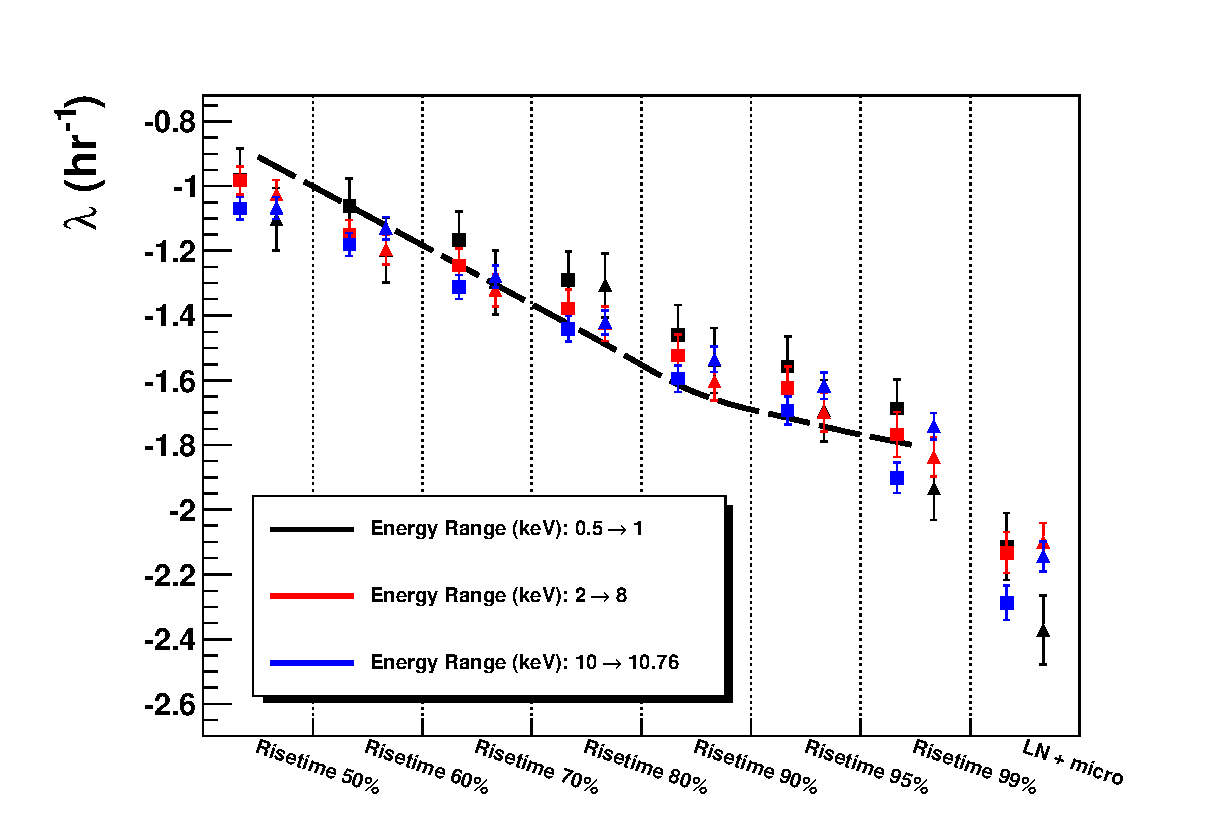
\includegraphics[width=0.7\textwidth]{BeforeAndAfterEvents}
				\caption[Rates calculated from the time difference between events in selected regions]
				{Rates calculated from the time difference between events in selected regions and events outside that region.  $\lambda$ is the raw parameter in the exponential fit ($\exp(\lambda t)$).The rates were calculated both forward
				in time (squares) and backwards in time (triangles) for different cut types.  The line drawn is an estimate of the 
				expected efficiency of the rise-time cuts using the $2\to8$~keV region, see text for details.}
				\label{fig:BeGeForBack}
			\end{figure}	
			
			\begin{table} \scriptsize
				\centering
				\renewcommand{\arraystretch}{0.68}
				\begin{tabular}{l  c  c  c  r@{$~\pm~$}l  c  c  c } 
				\toprule
					Cut & Range (keV) & Triggers & Direction & \multicolumn{2}{c}{Rate (cts/hr)} & $\chi^2$ & NDF & P-value  \\
				\midrule
				\multirow{6}{*}{Risetime 50\%}& \multirow{2}{*}{$0.5~\to~1$} & \multirow{2}{*}{166}	& B & -1.10 & 0.10 & 4.77 & 7 & 0.689\\
					& & & F & -0.98 & 0.09 & 2.81 & 7 & 0.902\\
				& \multirow{2}{*}{$2~\to~8$} & \multirow{2}{*}{651}	& B & -1.03 & 0.05 & 19.10 & 18 & 0.386\\
					& & & F & -0.98 & 0.04 & 13.48 & 20 & 0.856\\
				& \multirow{2}{*}{$10~\to~10.76$} & \multirow{2}{*}{1158}	& B & -1.07 & 0.03 & 39.84 & 45 & 0.690\\
					& & & F & -1.07 & 0.03 & 26.00 & 39 & 0.945\\
				\midrule
				
				\multirow{6}{*}{Risetime 60\%}& \multirow{2}{*}{$0.5~\to~1$} & \multirow{2}{*}{205}	& B & -1.20 & 0.10 & 7.52 & 6 & 0.275\\
					& & & F & -1.06 & 0.09 & 2.80 & 7 & 0.902\\
				& \multirow{2}{*}{$2~\to~8$} & \multirow{2}{*}{711}	& B & -1.20 & 0.05 & 23.24 & 18 & 0.182\\
					& & & F & -1.15 & 0.05 & 30.70 & 19 & 0.044\\
				& \multirow{2}{*}{$10~\to~10.76$} & \multirow{2}{*}{1292}	& B & -1.13 & 0.03 & 28.50 & 39 & 0.892\\
					& & & F & -1.18 & 0.04 & 19.85 & 36 & 0.987\\
				\midrule
				
				\multirow{6}{*}{Risetime 70\%}& \multirow{2}{*}{$0.5~\to~1$} & \multirow{2}{*}{242}	& B & -1.30 & 0.10 & 7.04 & 6 & 0.317\\
					& & & F & -1.17 & 0.09 & 3.23 & 7 & 0.863\\
				& \multirow{2}{*}{$2~\to~8$} & \multirow{2}{*}{769}	& B & -1.32 & 0.05 & 14.98 & 17 & 0.597\\
					& & & F & -1.24 & 0.05 & 24.93 & 18 & 0.127\\
				& \multirow{2}{*}{$10~\to~10.76$} & \multirow{2}{*}{1482}	& B & -1.28 & 0.03 & 31.32 & 36 & 0.691\\
					& & & F & -1.31 & 0.04 & 28.13 & 36 & 0.823\\
				\midrule
				
				\multirow{6}{*}{Risetime 80\%}& \multirow{2}{*}{$0.5~\to~1$} & \multirow{2}{*}{293}	& B & -1.31 & 0.10 & 3.56 & 5 & 0.615\\
					& & & F & -1.29 & 0.09 & 4.38 & 8 & 0.821\\
				& \multirow{2}{*}{$2~\to~8$} & \multirow{2}{*}{824}	& B & -1.43 & 0.05 & 11.13 & 15 & 0.744\\
					& & & F & -1.38 & 0.06 & 22.71 & 16 & 0.122\\
				& \multirow{2}{*}{$10~\to~10.76$} & \multirow{2}{*}{1628}	& B & -1.42 & 0.04 & 37.31 & 34 & 0.319\\
					& & & F & -1.44 & 0.04 & 26.58 & 34 & 0.814\\
				\midrule
				
				\multirow{6}{*}{Risetime 90\%}& \multirow{2}{*}{$0.5~\to~1$} & \multirow{2}{*}{350}	& B & -1.54 & 0.10 & 1.89 & 4 & 0.756\\
					& & & F & -1.46 & 0.09 & 4.15 & 7 & 0.762\\
				& \multirow{2}{*}{$2~\to~8$} & \multirow{2}{*}{884}	& B & -1.60 & 0.06 & 9.95 & 15 & 0.823\\
					& & & F & -1.52 & 0.06 & 27.90 & 15 & 0.022\\
				& \multirow{2}{*}{$10~\to~10.76$} & \multirow{2}{*}{1779}	& B & -1.54 & 0.04 & 33.90 & 32 & 0.376\\
					& & & F & -1.59 & 0.04 & 24.89 & 30 & 0.730\\
				\midrule
				
				\multirow{6}{*}{Risetime 95\%}& \multirow{2}{*}{$0.5~\to~1$} & \multirow{2}{*}{402}	& B & -1.69 & 0.09 & 2.74 & 4 & 0.602\\
					& & & F & -1.56 & 0.09 & 3.80 & 6 & 0.704\\
				& \multirow{2}{*}{$2~\to~8$} & \multirow{2}{*}{914}	& B & -1.70 & 0.06 & 10.25 & 14 & 0.744\\
					& & & F & -1.62 & 0.07 & 30.54 & 15 & 0.010\\
				& \multirow{2}{*}{$10~\to~10.76$} & \multirow{2}{*}{1872}	& B & -1.62 & 0.04 & 28.90 & 32 & 0.624\\
					& & & F & -1.69 & 0.04 & 23.45 & 27 & 0.661\\
				\midrule
				
				\multirow{6}{*}{Risetime 99\%}& \multirow{2}{*}{$0.5~\to~1$} & \multirow{2}{*}{457}	& B & -1.94 & 0.10 & 5.89 & 4 & 0.207\\
					& & & F & -1.69 & 0.09 & 1.94 & 5 & 0.858\\
				& \multirow{2}{*}{$2~\to~8$} & \multirow{2}{*}{976}	& B & -1.84 & 0.06 & 11.25 & 13 & 0.590\\
					& & & F & -1.77 & 0.07 & 24.01 & 14 & 0.046\\
				& \multirow{2}{*}{$10~\to~10.76$} & \multirow{2}{*}{1982}	& B & -1.74 & 0.04 & 24.28 & 28 & 0.666\\
					& & & F & -1.90 & 0.05 & 32.06 & 27 & 0.230\\
				\midrule
				
				\multirow{6}{*}{LN + micro}& \multirow{2}{*}{$0.5~\to~1$} & \multirow{2}{*}{526}	& B & -2.37 & 0.11 & 8.35 & 4 & 0.080\\
					& & & F & -2.11 & 0.10 & 1.92 & 4 & 0.751\\
				& \multirow{2}{*}{$2~\to~8$} & \multirow{2}{*}{1564}	& B & -2.10 & 0.06 & 11.87 & 11 & 0.374\\
					& & & F & -2.13 & 0.06 & 23.39 & 10 & 0.009\\
				& \multirow{2}{*}{$10~\to~10.76$} & \multirow{2}{*}{2054}	& B & -2.14 & 0.05 & 26.70 & 24 & 0.319\\
					& & & F & -2.29 & 0.05 & 29.52 & 22 & 0.131\\
				\bottomrule
				\end{tabular}


				\caption[Results of fits to time differences for events in selected energy ranges with different cuts]
				{Results of fits to time differences between events in selected energy ranges with different cuts.  
				The P-Value is the probability of observing this $\chi^{2}$ value or greater given the NDF. `B' and `F' correspond to backwards
				and forwards time differences, respectively.}
				\label{tab:BeGeForBackTable}			
			\end{table}

		\subsection{Time-energy correlations}
		\label{sec:BeGeTimeEnergyCor}

	Two-dimensional energy-time correlations were calculated by analyzing a time window around events occurring in a selected region.  As before, a set of events were selected within an energy range to be used as `trigger' events.  Given the time of a trigger event as a reference point, a two-dimensional energy vs.~time histogram was generated for all events occurring within a time window forwards and backwards around the reference.  The 2-d histograms for each trigger were then added together, producing a final intensity plot.  Any strong correlation between events in energy-time space should show up as having significant intensity in these figures.  The data used for this analysis had only LN fill cuts applied to avoid removing correlating events from the data set.
	
	To give an example of how this calculation works, the time-energy correlation between the \gersixeight~and \galsixeight~decays was analyzed.  The details of this decay chain are discussed in Section~\ref{sec:Ge68ProdPPC}, but a summary of the relevant points is given:  \gersixeight~internal to the crystal decays to \galsixeight, depositing 10.36~keV of energy $\sim90\%$ of the time via x-rays and Auger electrons.  \galsixeight~has a 68~minute half-life and decays via electron-capture $\sim10$\% of the time; 90\% of these decays are K-line captures and deposit 9.7~keV into the crystal.  We can therefore look for a time correlation by choosing the trigger region $10\to10.76$~keV and looking forwards and backward in time around the 9.7~keV decay region of \galsixeight~\cite{Schonfeld1994955}.  Results for 2211~triggers are shown in Figure~\ref{fig:BeGeGeCorrelation} where the intensity of the daughter decay is clear between 0 and 2~hours post trigger.  The rough expected count rate for the Ga K-capture decay is about $0.09\times2211 \sim 200$ which agrees with the results of the plot.  
	

			\begin{figure}
				\centering
				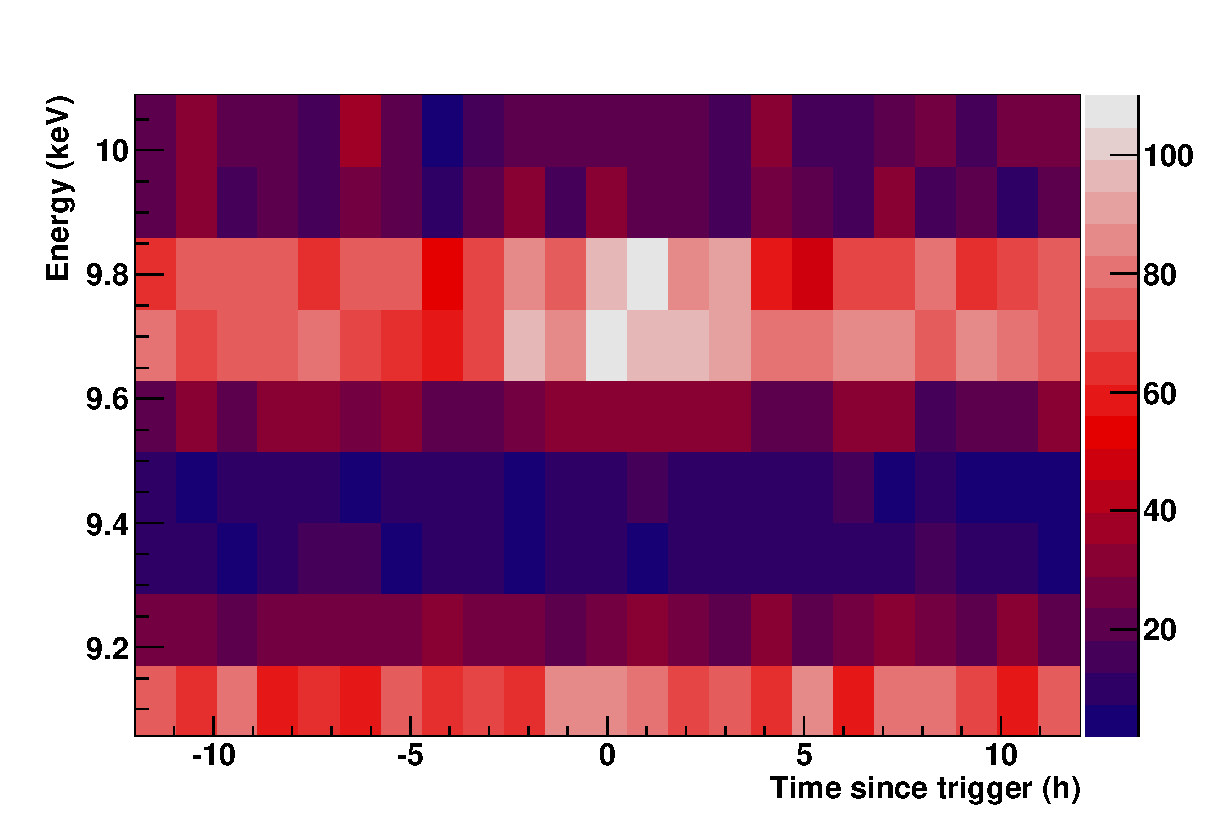
\includegraphics[width=0.7\textwidth]{GeCorrelationHighEnergy4}
				\caption[Time-energy correlation triggering on \gersixeight~decays.]
				{Time-energy correlation triggering on \gersixeight~decays (2211~triggers), z-axis is in counts.  The region intensity centered at 9.7~keV between 0 and 2~hours post trigger arises from the K-capture decay of the 
				\galsixeight~daughter.}
				\label{fig:BeGeGeCorrelation}
			\end{figure}	

	This analysis was applied to other trigger regions, including a region against threshold, $0.5\to1$~keV, and away from cosmogenic peaks, $2\to6$~keV.  The results are presented in Figure~\ref{fig:BeGeTimeEnergyCor} for an energy window from 0.5 to 8~keV, avoiding higher energies where the count rates from the \znsixfive~and \gersixeight~dominate the intensities.  The only apparent features in these plots are intensities at around 1.3~keV, which likely correspond to random coincidences with the \gersixeight~L-capture decay.  It is possible to integrate these 2-dimensional histograms along the time axis, producing an average energy spectrum around a trigger in the designated region.  By dividing by the number of triggers and the time of integration, one can compare the spectra from different trigger regions to identify any particular discrepancies.  This was done for all three regions presented in this section, integrating over $\pm12$~hours for the lower energy regions and $\pm3$~hours for the \gersixeight~K-capture region.  The results of this integration are shown in Figure~\ref{fig:BeGeIntegratedTimeEnergyCor}.  All of the trigger regions are consistent, except that the $10\to10.76$~keV trigger region demonstrates an enhancement in the \galsixeight~K-capture line.  This is to be expected since the average rate of the Ga decay should be higher centered on a trigger from the parent decay.

			\begin{figure}
				\centering
				\def\figwidth{0.83\textwidth}
				\def\plotname{CorrelationHighEnergy}	
				\subfigure[$0.5\to1$~keV]{
					\includegraphics[width=\figwidth]{NearTrigger\plotname2}
					\label{fig:\plotname5to1}
				}							
				\subfigure[$2\to6$~keV]{
					\includegraphics[width=\figwidth]{Test\plotname1}
					\label{fig:\plotname2to6}
				}			
				
				\caption[Time-energy correlations in selected regions.]
				{Time-energy correlations in selected regions with 575 triggers in the $0.5\to1$~keV region, 1200 in $2\to6$~keV. 
				The z-axes are in counts.}
				\label{fig:BeGeTimeEnergyCor}
			\end{figure}
	
	
			\begin{figure}
				\centering
				\def\figwidth{0.44\textwidth}
				\def\plotname{EnergyProjection0}	
				\subfigure[Low energy]{
					\includegraphics[width=\figwidth]{Low\plotname}
					\label{fig:Low\plotname}
				}							
				\subfigure[High energy]{
					\includegraphics[width=\figwidth]{High\plotname}
					\label{fig:High\plotname}
				}			
				
				\caption[Average energy spectra around triggers in selected energy regions.]
				{Average energy spectra around triggers in selected energy regions.  The $0.5\to1$ and $2\to6$~keV regions were integrated $\pm12$~hours around a trigger, the $10\to10.76$~keV region
				$\pm3$~hours.  As expected, there is a slight enhancement in the \galsixeight~K-capture peak for triggers in the \gersixeight~region.  The source of other enhancements at low energies has not been determined.}
				\label{fig:BeGeIntegratedTimeEnergyCor}
			\end{figure}	
			
			
		\subsection{Conclusions}
		\label{sec:BeGeTimeConclusions}			
		
	The search for time correlations in the data yielded results consistent with Poisson statistics, suggesting that the regions of the data sets tested are clean from events arriving in bursts or with defined frequency.  Additionally, the electronic noise of the detector remained constant throughout the counting runs.  The one significant deviation found resulted in the discovery of a class of events detailed in Section\ref{sec:BeGeElecCuts}, but the lack of other environmental information made it impossible to determine their origin.  For long-running experiments such as the \MJ~\minmod, the monitoring and control of the environment is critical for tracking down and explaining events that may appear in the data.  As the abilities of future experiments expand to include the unexplored regions enabled by ultra-low-energy thresholds, so too must the effort to ensure that these areas are fully understood.  
	
	%It should be noted that all these tests except the time difference measurement were insensitive to time correlations beyond their time windows (e.g.~8, 24~hours).    More powerful time-series analyses such as a Fourier or wavelet analysis could provide additional insight into the arrival information of events, 

	\section{Systematic error summary}
	\label{sec:BeGeSysError}
	
	The previous sections have discussed possible systematic errors in detail.  To summarize, systematic errors may arise from the following:
		\begin{itemize}
			\item Threshold drift 
			\item Contributions at low energy from non-Poisson processes (environmental noise)			
			\item Cut efficiencies (errors in the estimation of microphonics and rise-time cut efficiencies)
			\item Estimation of detector fiducial mass
		\end{itemize}
		
	The threshold drift can be estimated by considering that the $\sigma$ of the baseline (Section~\ref{sec:BeGeParsVsTime}) only varies by 0.1~mV.  Since the magnitude of the baseline is subtracted for every events, drifts over long time scales shouldn't affect the estimation of the energy on an event-by-event basis.  Therefore, we expect that the drift in threshold can be estimated using the $\sigma$ of the baseline, which corresponds to roughly 7~eV in energy units.  
	
	An upper limit on the contribution of a non-Poisson process to the count rate at $0.5\to1$~keV can be made by conservatively assuming that it must be less than or equal to the error on the measured rate in that region.  That is, the rate (after LN cuts) is measured as $0.172\pm0.007$ counts/hour in that region.  Therefore, a non-Poisson process could contribute $\leq4$\% to events in this region.  	
	
	The \emph{acceptance} efficiencies for the rise-time cuts have been estimated by performing a systematic analysis on the behavior of the cuts on peaks in the data.  At higher acceptance ($\geq70$\%), the estimated efficiencies are correct within 10\%.  This error is not explicitly taken into account, but the effect of the different cuts is studied during limit calculations (Section~\ref{sec:LimitsUnbinned}).  The error is biased since the efficiencies are always underestimated, meaning that limit estimations will be conservative.  The detector fiducial mass has been estimated as $0.346\pm0.0124$~kg, but the value of this has been conservatively assumed to be at the lower end of this error: 0.33~kg.  As with the rise-time efficiency underestimation, this will make limit calculations more conservative since a decrease in assumed mass reduces the sensitivity of a detector.  
	
			\begin{table} 
				\centering
				\begin{tabular}{p{0.4\textwidth}  c  p{0.35\textwidth}  } 
				\toprule
					Source & Estimate & Comments \\
				\midrule	
					Threshold drift & $\lesssim7$~eV & Estimated from baseline versus time measurements, negligible/ignored \\
					Non-Poisson process contribution & $\leq4$\% of counts & Possible `unknown background' contribution to $0.5\to1$~keV region.  \\			
					Rise-time cut efficiency error & $\lesssim10$\% & For efficiencies $\geq$70\%; effects of different cuts studied during limit calculations (Section~\ref{sec:LimitsUnbinned}) \\
					Fiducial mass error & 4\% & Error ignored, but mass conservatively assumed to be 0.33~kg\\

				\bottomrule
				\end{tabular}	
				\caption{Summary of estimation of systematic errors.}
				\label{tab:BeGeSysErrors}
			\end{table}
	\section{Conclusions}
     	\label{sec:BeGeConclusions}		
	
	During the counting runs presented here, the detector and electronics demonstrated good stability, running without significant intervention for almost half a year.  At the time of writing, data collection continues.  A robust analysis chain developed for a previous \ppc~detector at Soudan was applied to the distinct DAQ setup used for the modified \bege, demonstrating the adaptability required for use with the \MJ~\minmod.  Tools were developed to measure the rise-time of preamplifier traces with small signal-to-noise ratios, and the results can be applied to future detectors with similar or better capabilities including \ppc~detectors in the \minmod.  Future DAQ systems for the \minmod~will likely forego the use of spectroscopic amplifiers, opting for the simplicity afforded by directly digitizing the preamplifier output.  Therefore, the study of microphonics cuts based upon preamplifier traces must progress, though it is expected that the ability to differentiate between `real' events and those vibrationally induced will improve because the deviations in preamplifier traces should manifest more significantly.  The study of the rise-time cuts demonstrated the ability to cut slow-rise-time pulses, but also implied that further work must progress to establish the robustness of this technique near threshold.  Additionally, determining if other origins of slow pulses exist and how the distribution of these pulses depends on geometry and manufacturing requires further quantitative tests with other similar detectors.  The cuts and analysis of this data have readied it for further interpretation: possible sensitivities and exclusion limits are discussed in the following chapters.
